\documentclass[preprint]{aastex}

\usepackage[top=1in, bottom=1in, left=1in, right=1in]{geometry}
\usepackage{amsmath}
\usepackage{graphicx}
%\usepackage{mdwlist}
\usepackage{natbib}
\usepackage{natbibspacing}
\usepackage{enumitem}
\usepackage[font=small,justification=justified,singlelinecheck=false]{caption}
%\usepackage{subcaption}
\usepackage{float}
\setlength{\bibspacing}{0pt}
\setlength{\parskip}{0pt}
\setlength{\parsep}{0pt}
\setlength{\headsep}{0pt}
\setlength{\topskip}{0pt}
\setlength{\topmargin}{0pt}
\setlength{\topsep}{0pt}
\setlength{\partopsep}{0pt}
\setlength{\footnotesep}{8pt}
\pagestyle{empty}
\citestyle{aa}
%\usepackage[font=small]{caption}
\captionsetup[table]{labelsep=space}
\captionsetup[figure]{labelsep=space}

\newcommand{\Mycite}[1]{{\bf \cite{#1}}}
\newcommand{\Mycitet}[1]{{\bf \citet{#1}}}
\newcommand{\Mycitep}[1]{{\bf \citep{#1}}}
\newcommand{\Mycitealt}[1]{{\bf \citealt{#1}}}

\newcommand{\compress}{\vspace{-0.3in}}
\newcommand{\captionbaseline}{\renewcommand{\baselinestretch}{0.9}} 
\newcommand{\Caption}[4]{\vspace{#1}\renewcommand{\baselinestretch}{#2}\caption{#4}\vspace{#3}}

\setcounter{totalnumber}{1} % force only 1 figure per page

\def\kperp{k_{\bot}}
\def\kpar{k_{\|}}
\def\nwnh{{\sl NWNH}}

\newcommand{\simgt}{\stackrel{>}{_{\sim}}}
\def\kperp{k_{\bot}}
\def\kpar{k_{\|}}
\def\k{{\bf k}}
\def\sky{{\theta}}
\def\HI{{H{\small I }}}
\def\HII{{H{\small II }}}
\def\xHI{{x_{\rm\HI}}}

%project description 20 pages total

\begin{document}

%\title{Hydrogen Epoch of Reionization Array: Characterizing Cosmic Dawn}
\title{HERA: Illuminating Our Early Universe}
{\it For the Mid-Scale Science Projects category of the Mid-Scale
Innovations Program}

\begin{figure}[H]\centering
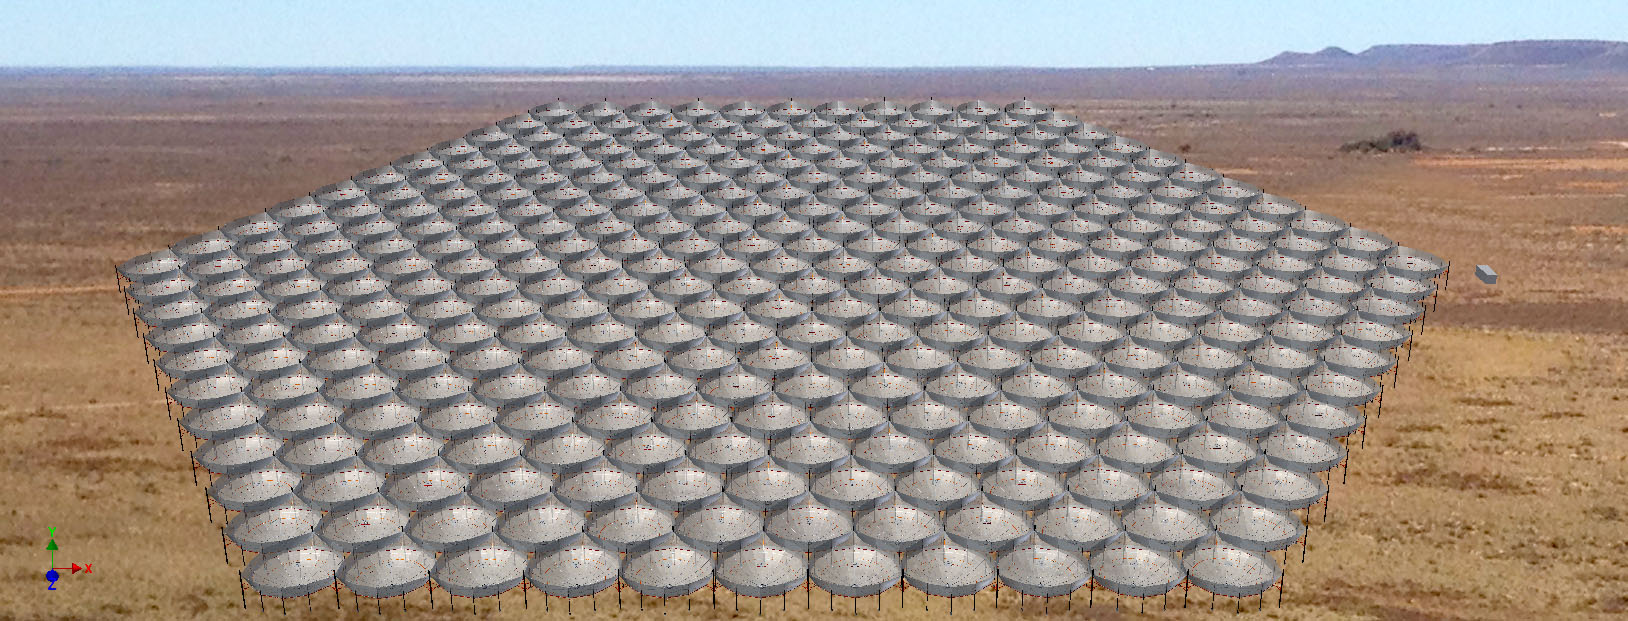
\includegraphics[width=6in]{plots/hera331perspect2.jpg}
\Caption{-0.1in}{0.9}{-0.1in}{\small
The proposed array of 331 14~m-diameter zenith-pointing dishes in the Karoo Radio Astronomy Reserve
in the Northern Cape of South Africa.}\label{fig:hera_array} \end{figure}

% Parsons, Carilli
% A statement of which of the four categories of MSIP is most appropriate
%for this proposal as the first sentence (see section II. Program Description).
%A. We propose HERA: next step in reionization roadmap
%B. Fulfill NWNH high-priority goals
%C. New understanding/techniques => faster, better, cheaper
%D. Brief summary of timeline: science along the way, major results before end-decade

\vspace{-0.4in}
\section{Overview of this Proposal} % 1 page ~ project summary? 

% I would really start out saying that this is a proposal to detect the EOR 21 cm
% at high enough significance to exclude models based on scale and redshift
% dependence of the power spectrum, plus map the brightest features.  The array
% itself is a consequence, not the driver, of the proposal.

The Hydrogen Epoch of Reionization Arrays (HERA) roadmap is a staged
plan to use the unique properties of the 21~cm ``spin-flip" line from neutral
hydrogen to probe our cosmic dawn, from the birth of the first 
stars and black holes through the full reionization of the primordial
intergalactic medium (IGM). During this epoch, roughly 0.1--1~Gyr after the Big Bang, 
the neutral hydrogen that pervades the Universe 
following recombination is warmed, and then reionized by the first luminous sources. 
The Universe is transformed from one dominated by simple,
linear evolution driven by gravity to an extraordinarily complex system with stars, black holes, and galaxies that
dramatically change the state of baryons in the Universe through widespread heating and reionization.
Direct observation of the large-scale structure of the primordial
IGM, and its evolution with time, via the \HI 21~cm line will
have a profound impact on our understanding of the birth of the first
galaxies and black holes, their influence on the surrounding gas,
and cosmology. 

HERA was ranked the ``{\it top priority in the Radio, Millimeter, and
Sub-millimeter category of recommended new facilities for mid-scale
funding}" as part of the {\it New Worlds, New Horizons of Astronomy
and Astrophysics} decadal survey (\citealt{astro2010}; hereafter
NWNH).  The HERA roadmap initially envisioned a series of radio
interferometers constructed throughout the decade. Phase I of this roadmap
incorporated existing instruments --- the Donald C. Backer Precision Array to Probe the Epoch of
Reionization (PAPER) and the Murchison Widefield Array (MWA) ---
aimed at characterizing foregrounds and laying the
groundwork for a statistical detection of the HI 21~cm signal through
the power spectrum.  A second-generation HERA instrument would measure
the evolution of the power spectrum, revealing details of the astrophysics driving
the birth and evolution of galaxies 
in the early Universe. A third-generation instrument would
directly image structures throughout reionization.

With a fraction of the funding recommended for HERA Phase I
in NWNH, the MWA and PAPER projects have made
major strides in developing techniques to disentangle
the reionization signal from the strong radio continuum foreground
emission.  These techniques, which are based on a new
understanding of the interplay of foreground and instrumental systematics
in the context of a three-dimensional cosmological intensity-mapping experiment,
have yielded a critical breakthrough.  As discussed below, {\bf we are now able to remove 
foregrounds to the limits of our sensitivity with these instruments},
and this is culminating in the first physically meaningful upper limits
on the power spectrum of 21~cm emission from reionization \Mycitep{parsons_et_al2013}\footnote{Throughout the proposal, we have indicated work by members of the present collaboration in bold.}
%PAPER
%and MWA are now performing deep science observations, with the potential to 
%obtain a nominal detection of the HI 21~cm signal within two years. 

% last sentence above could go - cc; agreed - JCP
% Carilli: I think the paragraph below is a bit repeditive. 
% In the interest of length, I have commented out and revised below

%Current generation 21~cm reionization experiments (LOFAR, MWA, PAPER) 
%are fully constructed and have been engaged in observations
%that will soon reach the sensitivity limits of these instruments.  Meanwhile,
%the principles that have yielded this breakthrough in foreground removal
%have given us new insight into how
%21~cm reionization experiments should be designed.  
%Based on these insights, we have developed a new 14~m diameter antenna element 
%that is optimized both for
%sensitivity and for minimizing foreground systematics.  
%Arranging these elements in a compact hexagonal grid yields an array that
%facilitates calibration, leverages proven foreground removal techniques, and is scalable

\begin{figure}[t]\centering
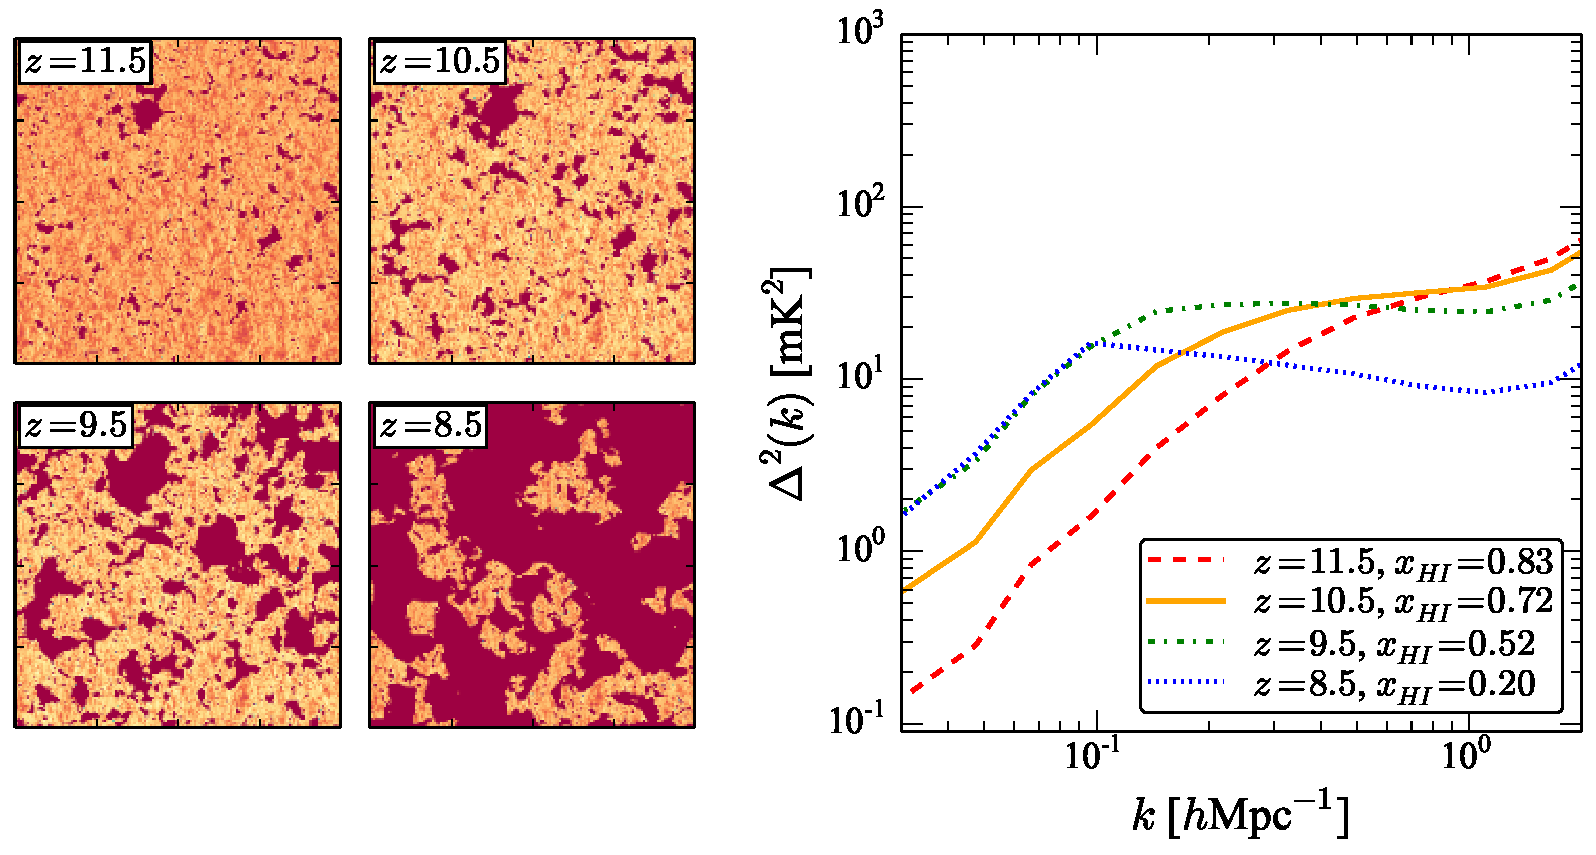
\includegraphics[height=2.5in]{plots/cubes/cubesAndPspecs.pdf}
\Caption{-0.2in}{0.9}{-0.1in}{\small 
Left: Simulated 21~cm brightness temperature distributions spanning $\sim 280 \times 280\,h^{-1}\textrm{Mpc}$.
at $z=11.5$, $10.5$, $9.5$, and $8.5$.
Right: Corresponding evolution of the 21~cm power spectrum.  HERA
characterizes the power spectrum in detail, as well as
providing images of the ionized bubbles (\S\ref{sec:science}).}
%\hline
\label{fig:EoRsims} \end{figure}
%to large collecting areas.

Using lessons learned from MWA and PAPER, 
we are now ready to build the instrument
that delivers HERA-II science at a cost that is substantially below the $\sim$\$60M envisioned in NWNH.
The proposed HERA-331 experiment is based on
a new 14~m diameter antenna element we have developed that is
optimized both for sensitivity and for minimizing foreground systematics.  
A compact hexagonal array of these elements 
improves sensitivity by nearly two orders of magnitude 
over the PAPER and MWA, and covers a wider frequency range (50 to 225~MHz).
This design facilitates calibration, leverages proven foreground removal techniques, and is supports
multiple approaches to reionization studies. 
Construction proceeds in two stages, allowing both for technical improvements and the delivery of 
key science throughout the project period: 

\begin{itemize}[noitemsep,nolistsep]

% JCP: do we have any consistency w.r.t. hyphens? HERA 127 vs. HERA-127
\item HERA~127: A 127-element hexagonal array, deployed at the
the end of project year 2, measures the rise and fall of the
21~cm reionization power spectrum from $z = 7$ to 12. These results tightly
constrain the evolution of the IGM neutral fraction, determining
the timing and duration of reionization. %in particular during epochs that are difficult or impossible to
%probe with other techniques.

\item HERA~331: A 331-element hexagonal array, deployed at the end of project year 3,
measures fluctuations in the 21~cm signal over a variety of spatial
scales to determine the nature and distribution of the first galaxies
that dominate cosmic reionization. HERA~331 extends precision
power-spectrum observations back to the pre-reionization epoch ($z \sim 20$), 
when the first stars and black holes warm the primordial IGM. HERA-331 can also potentially 
image the largest structures in the primordial
IGM --- a task previously only considered possible with third-generation
instruments. 

% ARP: these designs already said below
%Ultimately, HERA-331 will have the sensitivity to
%image directly the largest scale structures in the IGM during reionization.
\end{itemize}

\noindent
This proposal is a self-contained package for delivering the core of HERA-II science,
including telescope development, construction, observing, data analysis,
and scientific products for each stage of the project.  
This approach minimizes
risks associated with external funding contingencies while encouraging
collaborators to leverage resources for augmenting HERA's science.


%  ___     _                 
% / __| __(_)___ _ _  __ ___ 
% \__ \/ _| / -_) ' \/ _/ -_)
% |___/\__|_\___|_||_\__\___|


% Science currently at 5.5 pages.  

\compress
\section{Scientific Justification and Intellectual Merit} %total = 8 pages

\begin{figure}[t]\centering
%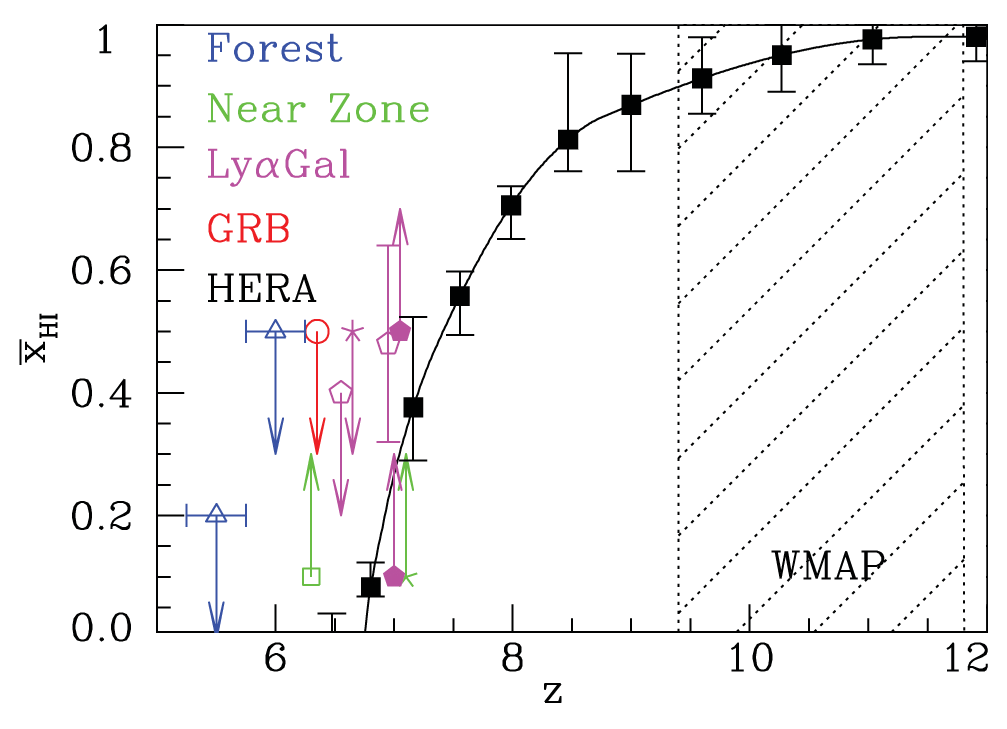
\includegraphics[height=2.25in]{plots/constraints_crop.pdf}
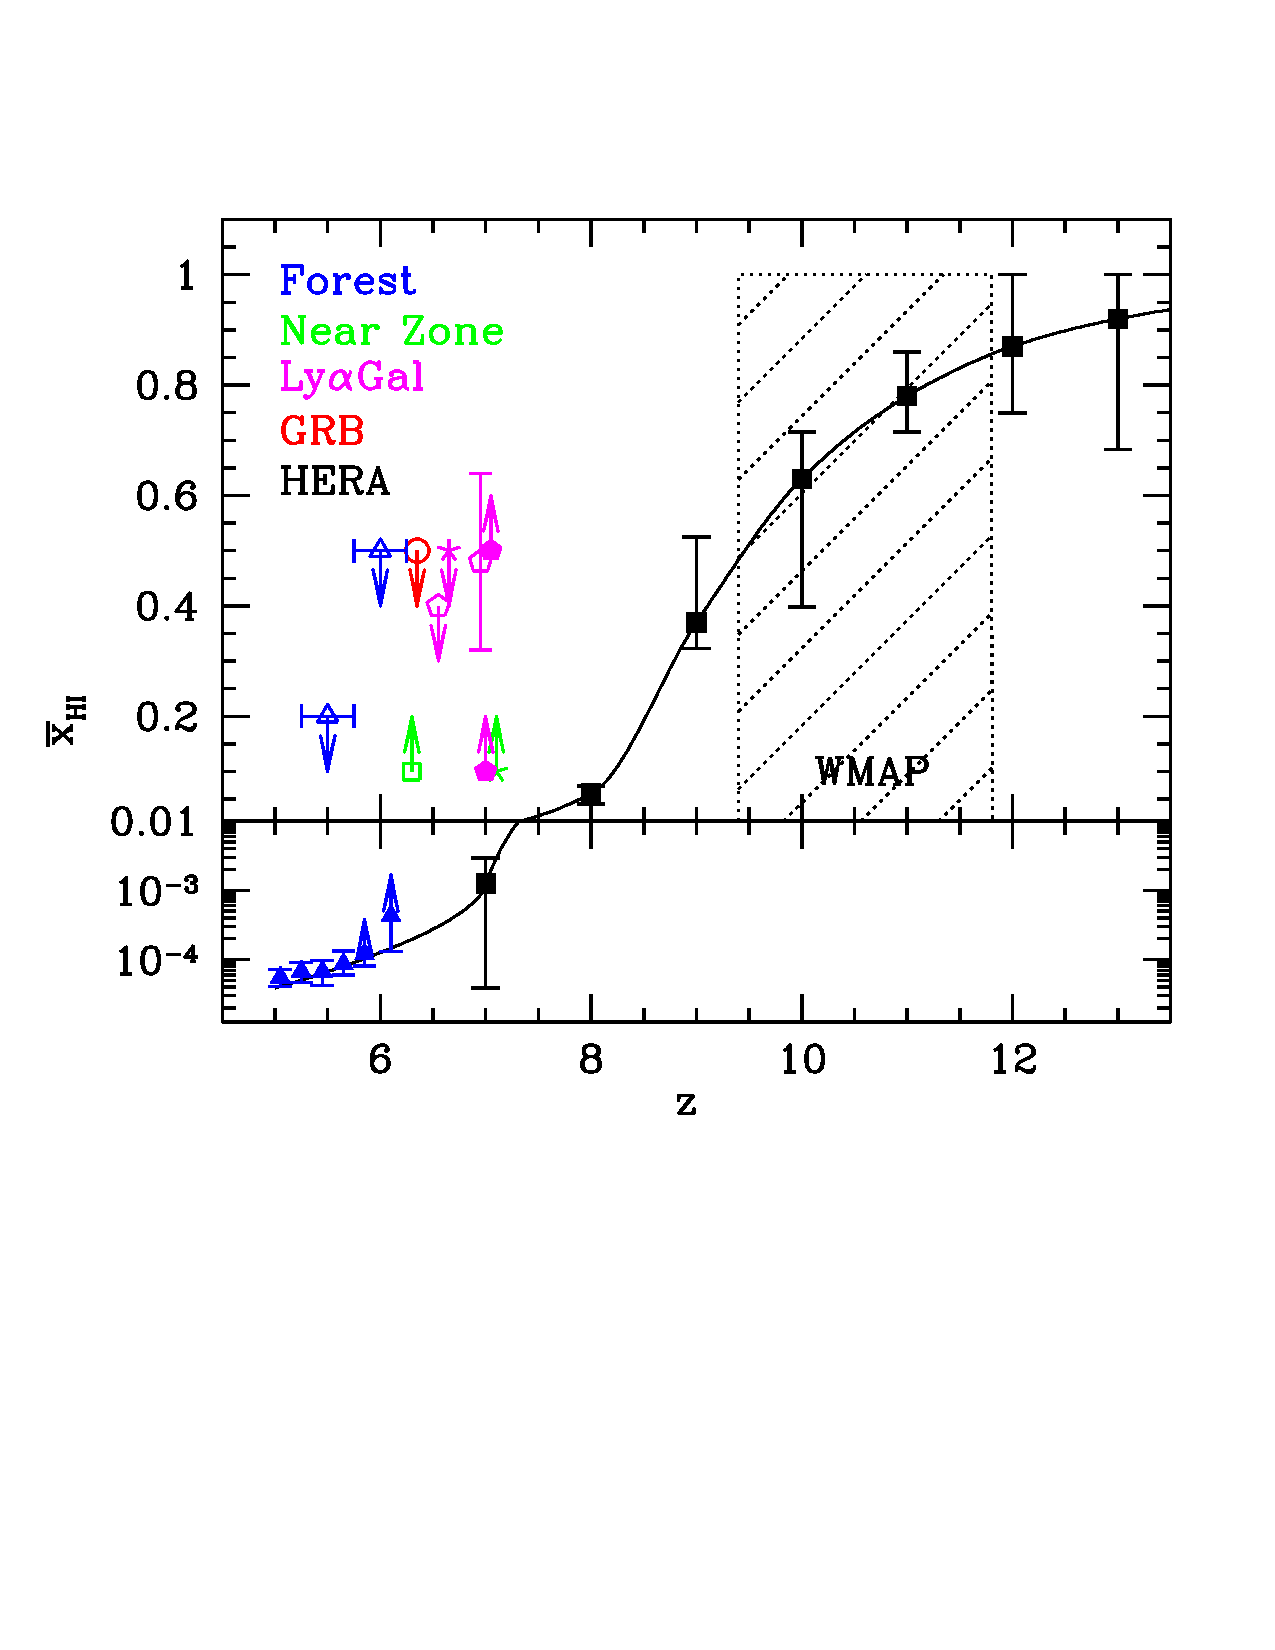
\includegraphics[height=2.25in,trim=0.8cm 9cm 1.75cm 3.6cm,clip]{plots/IonizationHistory/HERA331_ion_hist.pdf}
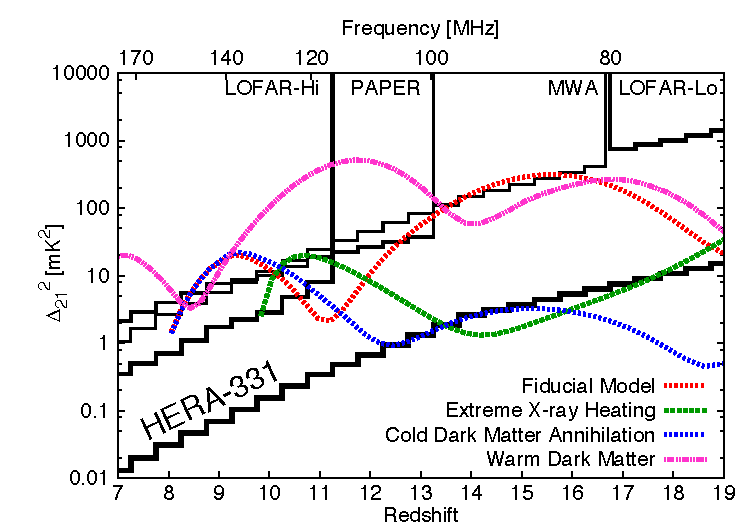
\includegraphics[height=2.25in]{plots/Xray/HERA_II_compare_kp1_whoriz_20pt.pdf}
\Caption{-0.1in}{0.9}{-0.1in}{\small
Left:
Existing
constraints on neutral fraction ($\xHI$) versus redshift (adapted from \citealt{robertson_2013}), along with
predicted HERA-331 constraints (black markers)
%assuming that $\xHI$ decreases versus redshift
for a fiducial
reionization history (black line).
At $z>8$,
21~cm emission may be the only precise probe of $\xHI$.
Right: At lower frequencies, HERA probes
pre-reionization physics at the end of the Dark Ages. Plotted are power spectrum amplitudes (at $k =
0.15h$~Mpc$^{-1}$) for various IGM heating models \Mycitep{mesinger_et_al2013},
with predicted sensitivities.
}\label{fig:x_i_vs_z} \end{figure}


%\subsection{Introduction}    % 1 page + 1 fig = simulated Tb cube + PS evolution
% Furlanetto, Carilli

%i.physical concepts: reionization and dark ages
%ii. Current knowledge: various constrai	nts, 1st galaxy studies...
%iii. Important role of 21~cm studies highlighted in NWNH
%a. Typical ideal sim results: T_B vs. z 'cube' and corresponding power spectrum evolution (Fig)
%b. introduce some of the important parameters/processes explored: when? how? bubble scale? sources? inside out? [much of this could be left for below?)
%c. reemphasize that current knowledge is nil, yet demand is high
%d. emphasize unique (only?) probe of dark ages

The {\it cosmic dawn}, the period beginning with the birth of the first stars and culminating with the full
reionization of the IGM 
%SF: Changed time period again
$\sim 1$~Gyr later, represents one of the last unexplored phases in cosmic history. 
This period is rich in both astrophysical and cosmological phenomena. 
The characteristics of the IGM depend on the cosmic density field, the first galaxies (e.g., their typical masses and 
clustering), their constituents (e.g., exotic Pop. III 
stars, more normal stars, stellar remnants, or supermassive black holes), their ultraviolet luminosities (which affect
the IGM ionization and thermal states), the efficiency and abundance of X-ray sources (which affect IGM temperature), 
and cosmological effects like the relative velocity of baryons and dark matter. 
Exploring these early structures, and their interplay with their environment was one of the top three ``{\it priority science objectives chosen by 
the [NWNH] survey committee for the decade 2012-2021.}"

% I have revised below, in light of Fan's comment that we need to highlight how 21~cm fits into the broader 
% picture of study of F(HI) and first galaxies

Study of the formation of the first galaxies and their influence on the primordial IGM, is 
among the highest priorities in modern astronomy, 
and a primary driver for many future large telescopes.  Recent measurements from the {\it Hubble Space Telescope} 
have pinned down the bright end of the galaxy luminosity function 
at $z \la 8$ \citep{bouwens_et_al2010, schenker_et_al2013} and have detected a few sources at even greater 
distances \citep{ellis_et_al2013, oesch_et_al2013}. Still, a complete census of the galaxies required for
reionization requires deep observations with, e.g., JWST and ALMA, to reveal the fainter end of the luminosity function. 
In parallel, a number of indirect techniques have been used to constrain the evolution of the neutral fraction
with redshift, although predominantly at the end of reionization. Figure~\ref{fig:x_i_vs_z} summarizes 
these results, including: 

\begin{itemize}[noitemsep,nolistsep]

\item Observations of resonant scattering of Ly$\alpha$ by the neutral IGM toward
distant quasars (the `Gunn-Peterson' effect) \citep{fan_et_al2006}.

\item The demographics of Ly$\alpha$ emitting  galaxies \citep{schenker_et_al2013, treu_et_al2013,Faisst_et_al2014}.

\item The Ly$\alpha$ absorption profile toward the most distant quasar ($z = 7.1$) \citep{bolton_et_al2011}.

\item Measurements of the optical depth to reionization based on CMB temperature fluctuations \citep{planck_et_al2013}
and large scale polarization anisotropies \citep{page_et_al2007}.

\item Secondary temperature fluctuations generated by the kinetic Sunyaev-Zel'dovich effect (\citealt{zahn_et_al2012}; \Mycitealt{mesinger_et_al2012}). 

\end{itemize}
\noindent
Results from these observations suggest a substantially neutral IGM as late as $z \sim 7$ (with the fractional $HI$ ionization rate as high as $x_{HI} \sim 0.5$), with a tail of ionization extending to high 
redshift ($z \sim 15$).  Unfortunately, these methods (while extremely informative), have limited 
reach as probes of reionization itself. In particular:
(1) probes using Ly$\alpha$ emission can study only the tail-end of reionization, 
due to the extreme optical depth of that transition; (2) inferences from galaxy populations require strong assumptions 
regarding stellar populations, the escape fraction of UV photons from the galaxies, the undetected source population, 
and IGM clumping; and (3) the CMB provides only an integral measure of ionization back to recombination. 
Moreover, many of these indirect observations require substantial modeling and in cases appear to be
in tension with one another, underscoring the difficulty of
their interpretation and the complexity of the reionization process.

The 21~cm ``spin-flip" transition of  neutral hydrogen has been recognized as potentially the most powerful probe 
of the cosmic dawn \Mycitep{morales_wyithe2010, furlanetto_et_al2006}, as emphasized in NWNH: 
``{\it 
%SF: Is this quote from the RMS panel?  If so, does it appear in the final report?
The panel concluded that  to explore the discovery area of the epoch of reionization, it is most important to 
develop new capabilities to observe redshifted 21~cm \HI emission, building on the legacy of current projects and 
increasing sensitivity and spatial resolution to characterize the topology of the gas at reionization.}"  Because 
our Universe was almost entirely neutral before reionization, the HI 21~cm line provides a direct method to image 
the evolution of the primordial IGM, opening a unique window into the complex astrophysical interplay between the 
first luminous structures and their surroundings. Moreover, because of the cosmological redshift, we can associate 
the signal at each observed frequency with a particular emission time (or distance) and reconstruct a complete 
three-dimensional picture of the time evolution of large scale structure during this key epoch in 
observational cosmology. 
%SF: Personally I feel like the following is an exaggeration that could rub some people the wrong way!
%The direct observation of the primordial IGM via the HI 21~cm line would be an achievement comparable in importance 
%to the detection of anisotropies in the CMB.

\begin{figure}[t]\centering
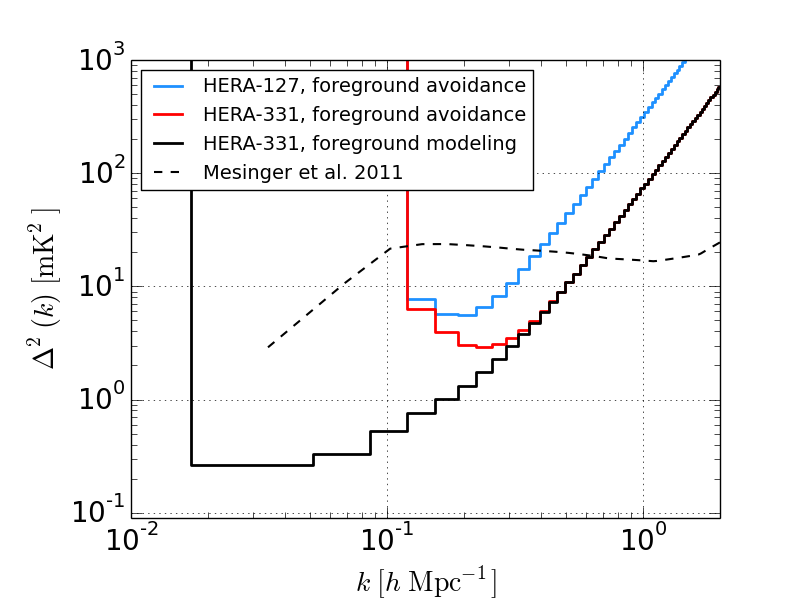
\includegraphics[height=2.25in]{plots/Pspec/eor_pspec_2014.png}
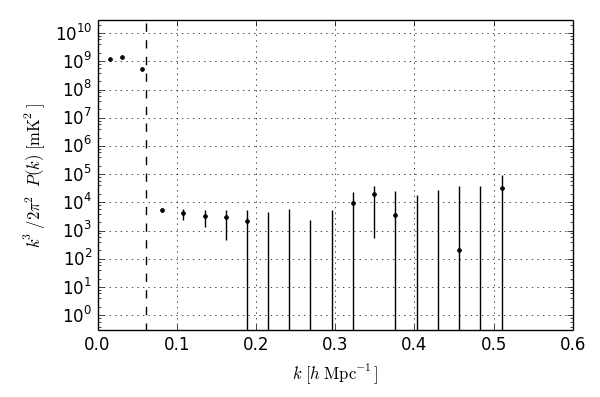
\includegraphics[height=2.25in]{plots/Pspec/pk_k3pk.png} 
\Caption{-0.1in}{0.9}{-0.2in}{\small Left: HERA's power-spectrum sensitivity (solid)
relative to a fiducial ionization model (dotted line; $\xHI=0.37$, $z=9.0$).
Sensitivities reflect staged array size and
improving analysis software that expands the range
of modes free of foreground systematics.
Right: The current best upper limit on the 21~cm reionization power spectrum,
obtained with a 32-element PAPER deployment \Mycitep{parsons_et_al2013}.  These upper limits
constrain the brightness temperature of the IGM at $z\sim8$, showing
a departure from adiabatic cooling presumed to be indicative of X-ray heating.
}\label{fig:eor_pspec}
\end{figure}


%\begin{figure}[t]\centering
%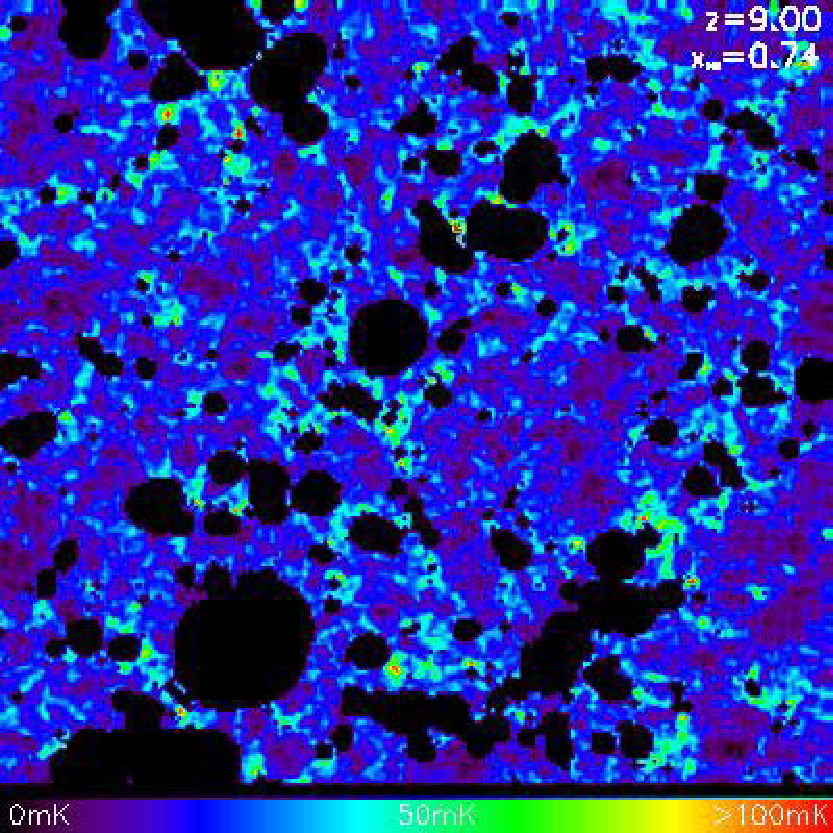
\includegraphics[width=0.23\textwidth]{plots/Pspec/z9sim.pdf}
%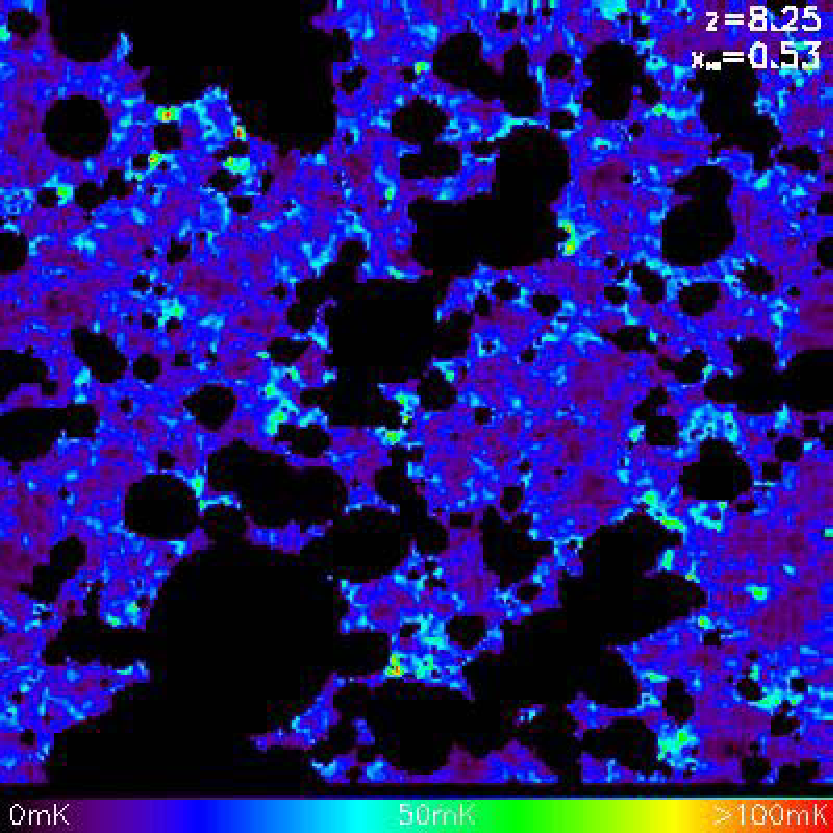
\includegraphics[width=0.23\textwidth]{plots/Pspec/z8sim.pdf}
%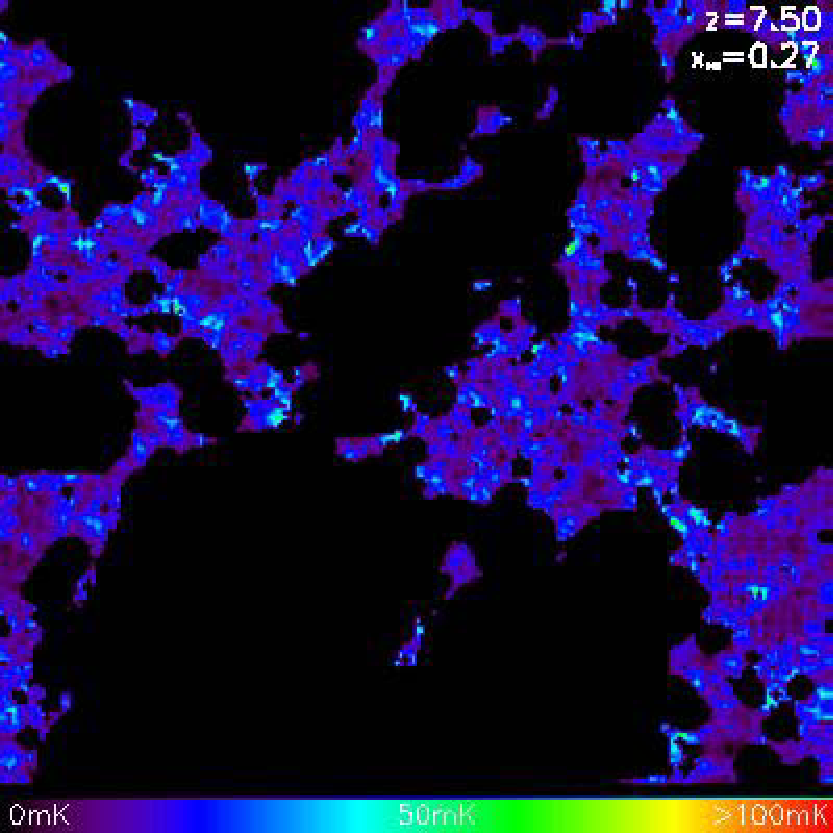
\includegraphics[width=0.23\textwidth]{plots/Pspec/z75sim.pdf}
%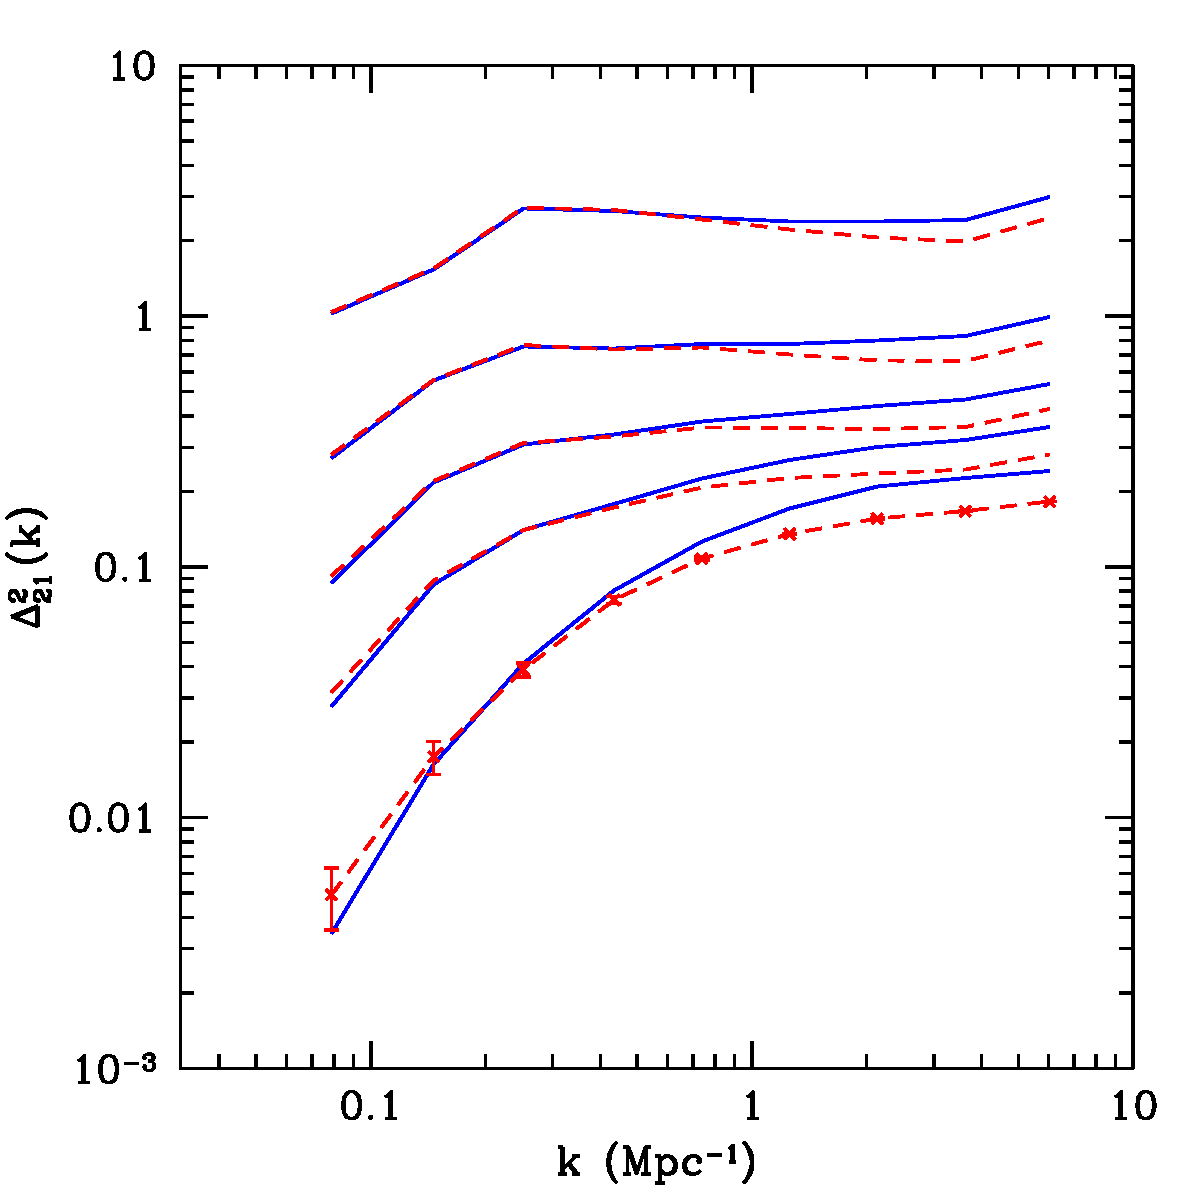
\includegraphics[width=0.23\textwidth]{plots/Pspec/pspecEvolve.pdf}
%\Caption{-0.2in}{0.9}{-0.2in}{\small 
%First three panels from left: simulated $21\,\textrm{cm}$ brightness temperature distributions at $z=9$, $8$, and $7.5$.  Rightmost panel: Evolution of the $21\,\textrm{cm}$ power spectrum from $z=9.25$ to $z=7$.  HERA will characterize the power spectrum in detail (Section \ref{sec:science}) as well as provide images of the ionized bubbles (Section \ref{sec:science}).
%}\label{fig:EoRsims} \end{figure}

Decades of effort have gone into modeling the complex astrophysics of reionization
(e.g. \citealt{shapiro_giroux1987, haiman_loeb1997}; \Mycitealt{furlanetto_et_al2004, santos_et_al2010}). Figure \ref{fig:EoRsims} shows a 
simulation of the expected evolution of the HI 21~cm signal during reionization \Mycitep{mesinger_furlanetto2007}. Fluctuations in the signal initially 
rise above those expected from the cosmic density field due to the growth of ionized bubbles on a characteristic 
scale of a few to 10~arcmin. This scale is set by the clustering of early galaxy formation, as well as by 
propagation effects through the IGM. The signal then declines as the IGM becomes fully ionized.  These theoretical 
models of the reionization process are sophisticated and appear to be well-understood, but they are not 
predictive tools. Instead, they provide a mapping between the largely unknown galaxy populations and observables 
like the 21~cm transition. As such, the key questions about the cosmic dawn era remain poorly understood.  When 
did reionization occur, and over what timescale?  What objects dominated the radiation field?  How were the 
objects distributed?  What were the most important feedback mechanisms in the transition from the first stars to
first galaxies, and how did they affect these populations?  {\it HERA provides the key measurements needed 
to advance our understanding of early galaxy formation and cosmic reionization.}
%JCP: The above paragraph is very good.

%Figures: F(HI) vs z;  HI Tb cube + PS evolution


\compress
\subsection{Science From Reionization and Cosmic Dawn} % 4 pages total examples using hera 331, plus a number of figures
\label{sec:science}

\begin{figure*}[t]\centering
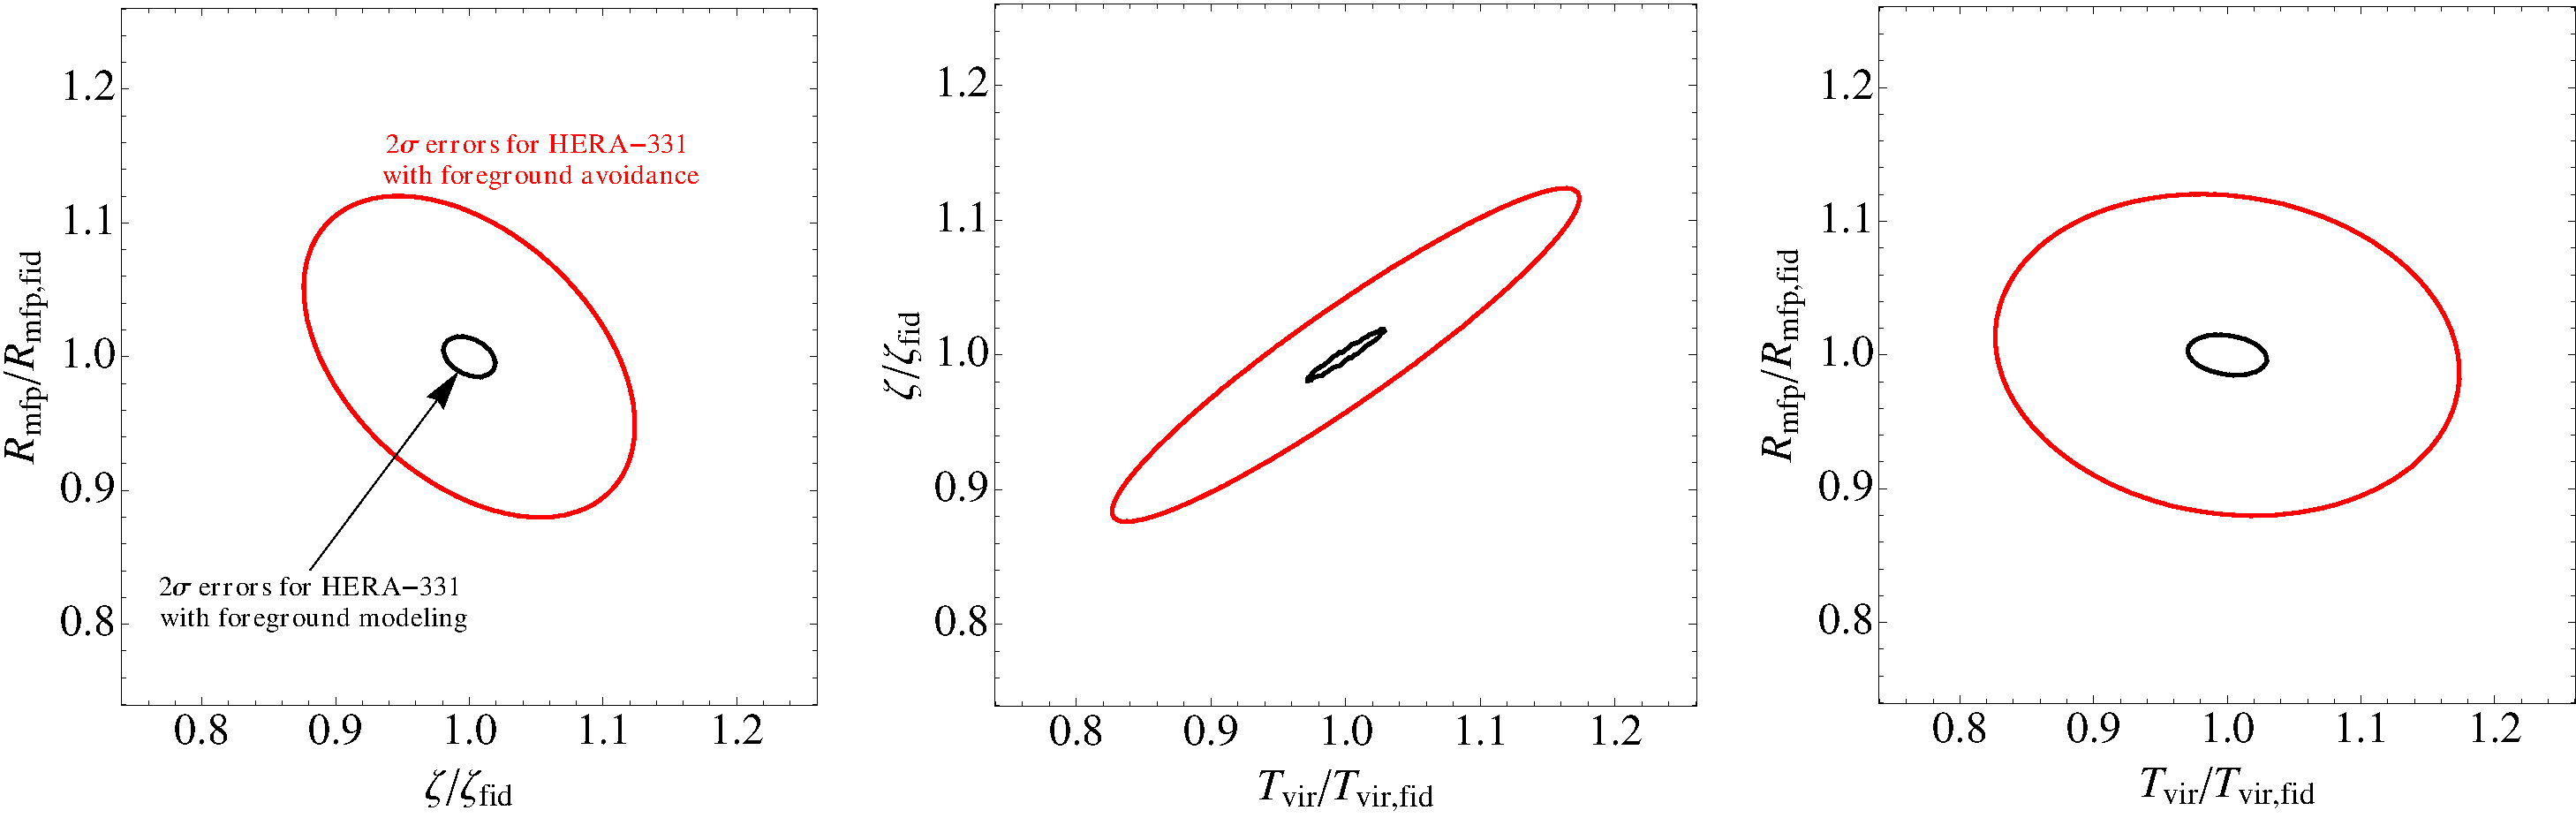
\includegraphics[width=\textwidth]{plots/Pspec/OPTMIDellipses.pdf}
\Caption{-0.3in}{0.9}{-0.15in}{\small
Pairwise $2\sigma$ error ellipses for $T_{\rm vir}$, $\zeta$, and $R_\textrm{mfp}$, in each case divided by their fiducial values.  HERA-331 projections using existing foreground avoidance techniques are shown in red, while projections using more advanced foreground modeling techniques are shown in black.  The former represent $\sim 5\%$ constraints, while the latter represent $\sim 1\%$ constraints.\label{fig:ErrorEllipses}}
\end{figure*}


As a high-sensitivity instrument with broad frequency coverage, HERA can
paint an uninterrupted picture of the evolution of the IGM through reionization and into the era of the cosmic dawn.
This capability leverages the coupling of
21~cm emission to the properties of the first galaxies that
are inaccessible through other means, making it be transformative for
studying the imprint of the very first galaxies in the Ly-$\alpha$ and X-ray backgrounds.
Figure~\ref{fig:x_i_vs_z} illustrates how HERA
determines the ionization history of our universe much more precisely,
and over a wider redshift range (thus at higher neutral fractions), than is possible with other existing techniques.
These measurements propel us beyond characterizing the timing and duration of reionization and into a regime
of asking detailed astrophysical questions, such as which galaxies dominate the integrated UV luminosity density, what the escape fraction
of UV photons is in early galaxies, and how feedback from early star formation affects low-mass galaxies and
the integrated  global ionization profile versus redshift.
At earlier epochs ($z \sim 15$ to 20), the sensitivity of the 21~cm line
to the IGM temperature provides a unique probe of processes that warm the neutral IGM during the cosmic dawn.
HERA has the frequency coverage and
sensitivity to study these earliest phases of star and black hole formation -- an epoch that may be otherwise
untestable, even with JWST.

%\compress
%\subsubsection{Detecting and characterizing the power spectrum}
%\emph{ii. PS sensitivity at fixed z: 127, 331 (Fig)}
% Pober, Dillon

{\bf Power Spectrum Detection}. A season of observing with HERA-127 yields high-significance constraints on the 21~cm power
spectrum across a wide range of wavenumbers and redshifts \Mycitep{pober_et_al2014}.  
Figure \ref{fig:eor_pspec} shows a $z=9$ power spectrum modeled by the 21~cmFAST software \Mycitep{mesinger_et_al2011},
along with $2\sigma$ HERA sensitivities.  Using a proven ``foreground avoidance" approach (see \S\ref{sec:Lessons})
we find that
HERA-127 achieves a $> 10\sigma$ detection over a broad range of redshifts.
Subsequent observing with HERA-331 boosts this to $>25\sigma$, as described in Table \ref{tab:signif}.  With detailed foreground modeling techniques
developed for the MWA, the overall significance rises to $90\sigma$,
along with new access to smaller $k$ modes and therefore qualitatively different physics.
%SF: I think this would go better in the next subsection (or can be left out)
%Such a high sensitivity measurement would also allow one to go beyond constraining parameters,
%testing rather than assuming the underlying theoretical framework

%\compress
%\subsubsection{Astrophysical parameters from the power spectrum}
%\emph{iii. Various covariance analyses: constraints on different physical processes (Liu/Pober analysis). but
%please -- keep this down to a couple of incisive figures and fiducial models. wall paper doesn't sell very well. }
% Liu, Pober, Dillon

{\bf Constraining Model Parameters}. Power spectrum measurements with HERA-331 are sensitive enough to place strict constraints on theoretical models of
reionization and even to test the fundamental assumptions of those models.  Within the standard framework,
three terms determine the major features of the power spectrum: $\zeta$, the efficiency at which galaxies
release ionizing photons  into the IGM; $T_{\rm vir}$, the minimum virial temperature of halos that produce
ionizing photons; and $R_{\rm mfp}$, the mean free path of ionizing
photons in the IGM (determined by the abundance of optically thick clumps).  Existing
observations limit the values of these parameters to within an order-of-magnitude at best.
Figure \ref{fig:ErrorEllipses} shows that we expect
HERA-331 power spectrum observations to constrain them to better
than 5\% using proven foreground avoidance techniques, with even stronger constraints from
explicit foreground modeling \citep{pober_et_al2014}.


% Jacobs
%\compress
%\subsubsection{Imaging HI}
%iv. Imaging large scale structure: simulation (Fig)
{\bf Imaging HI}. With a nearly completely sampled aperture over 300~m across, HERA has the collecting area of Arecibo, but
with $500\times$ the survey speed and sufficiently high sensitivity to image reionization directly.  After 100 hours on a
single field (achievable in 200 nights), HERA reaches a surface brightness sensitivity
of 50~$\mu$Jy/beam (synthesized beam FWHM $\sim 24'$) compared to the brightness temperature fluctuations of up to 400~$\mu$Jy/beam in typical reionization models.
Noise and foreground residuals are limiting factors.  Fortunately, many of the same foreground avoidance and modeling schemes used for power spectrum estimation can also be applied to imaging.  In Figure \ref{fig:imaging} we demonstrate the
resultant sensitivity of imaging in a foreground avoidance scheme, assuming a conservative 1~MHz of effective bandwidth, corresponding to 12~Mpc along the line of
sight.  The brightest structures in the $z=8$ input simulation are detectable at the SNR$>10$ level.
%SF: Is it useful to say how common such features are?  (If we know.)

% \begin{figure}[t]\centering
% 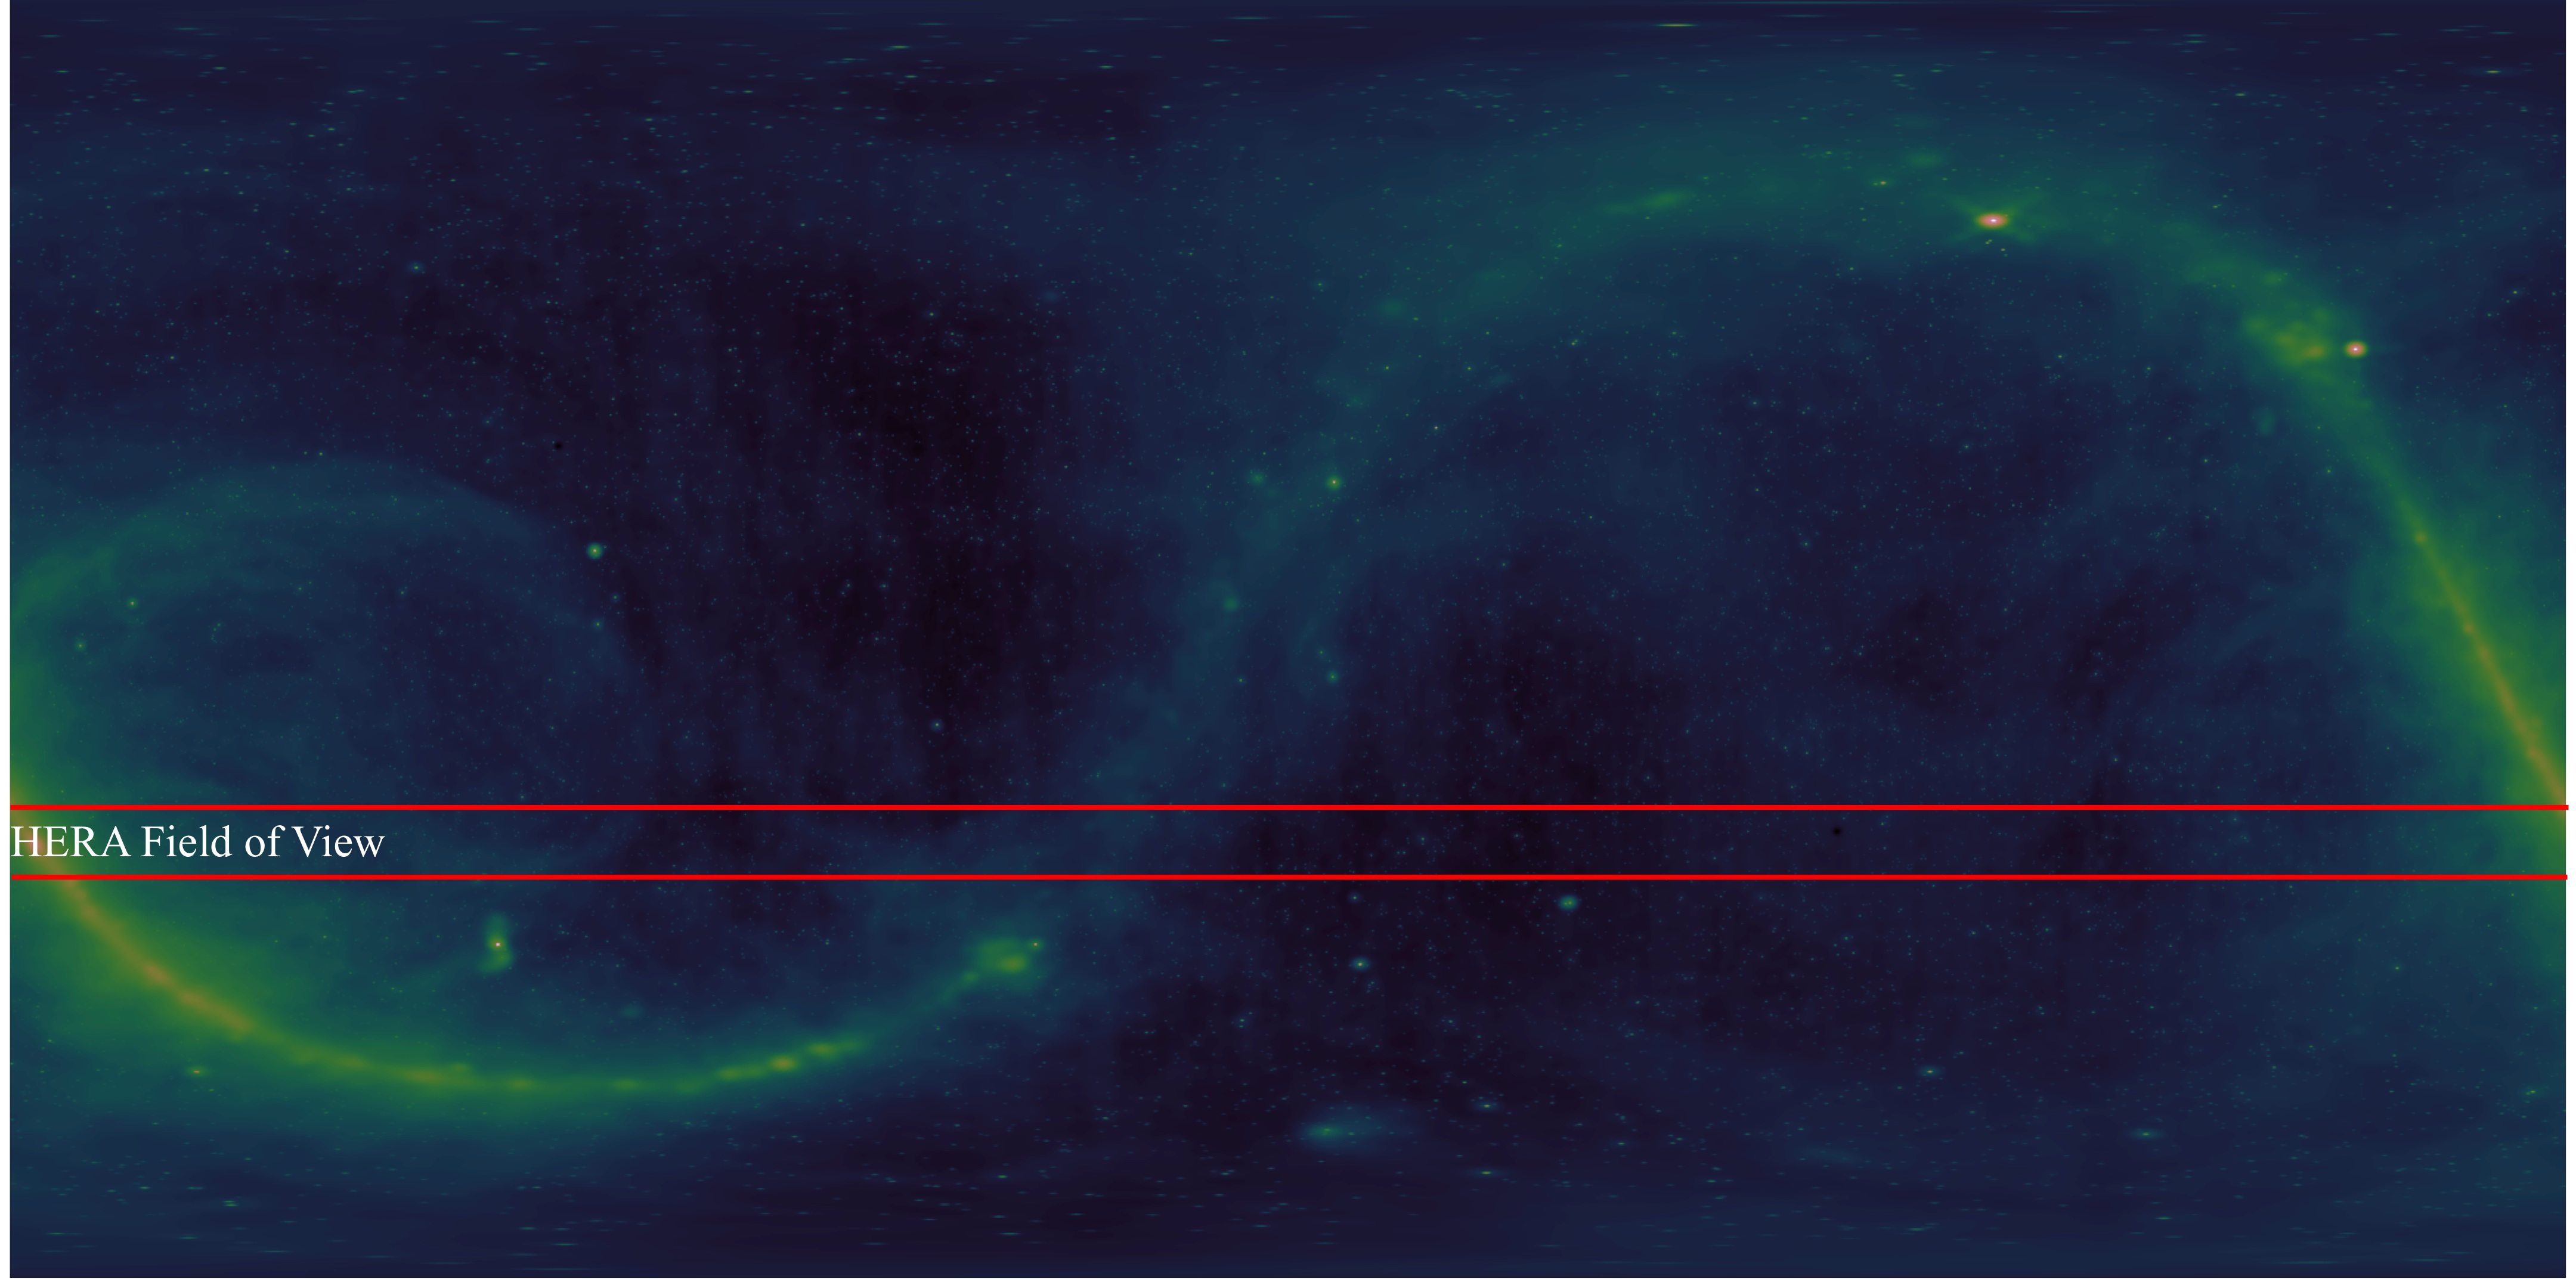
\includegraphics[width=\textwidth]{plots/Imaging/HERA_FoV.jpg}
% \Caption{-0.2in}{0.9}{-0.2in}{The HERA stripe.  At 150MHz ($z=8.5$) the HERA field of view is 8\arcdeg.  With a nearly completely sampled aperture over 300m across, HERA will have the collecting area of Arecibo but with 500x the survey speed. Each night it will drift scan 2600 square degrees for a survey volume of 50 $Gpc^3$.  The stripe includes the GOODs south field, one of the best studied regions of sky. \label{fig:HERA_FoV}}
% \end{figure}

\begin{figure}[t]\centering
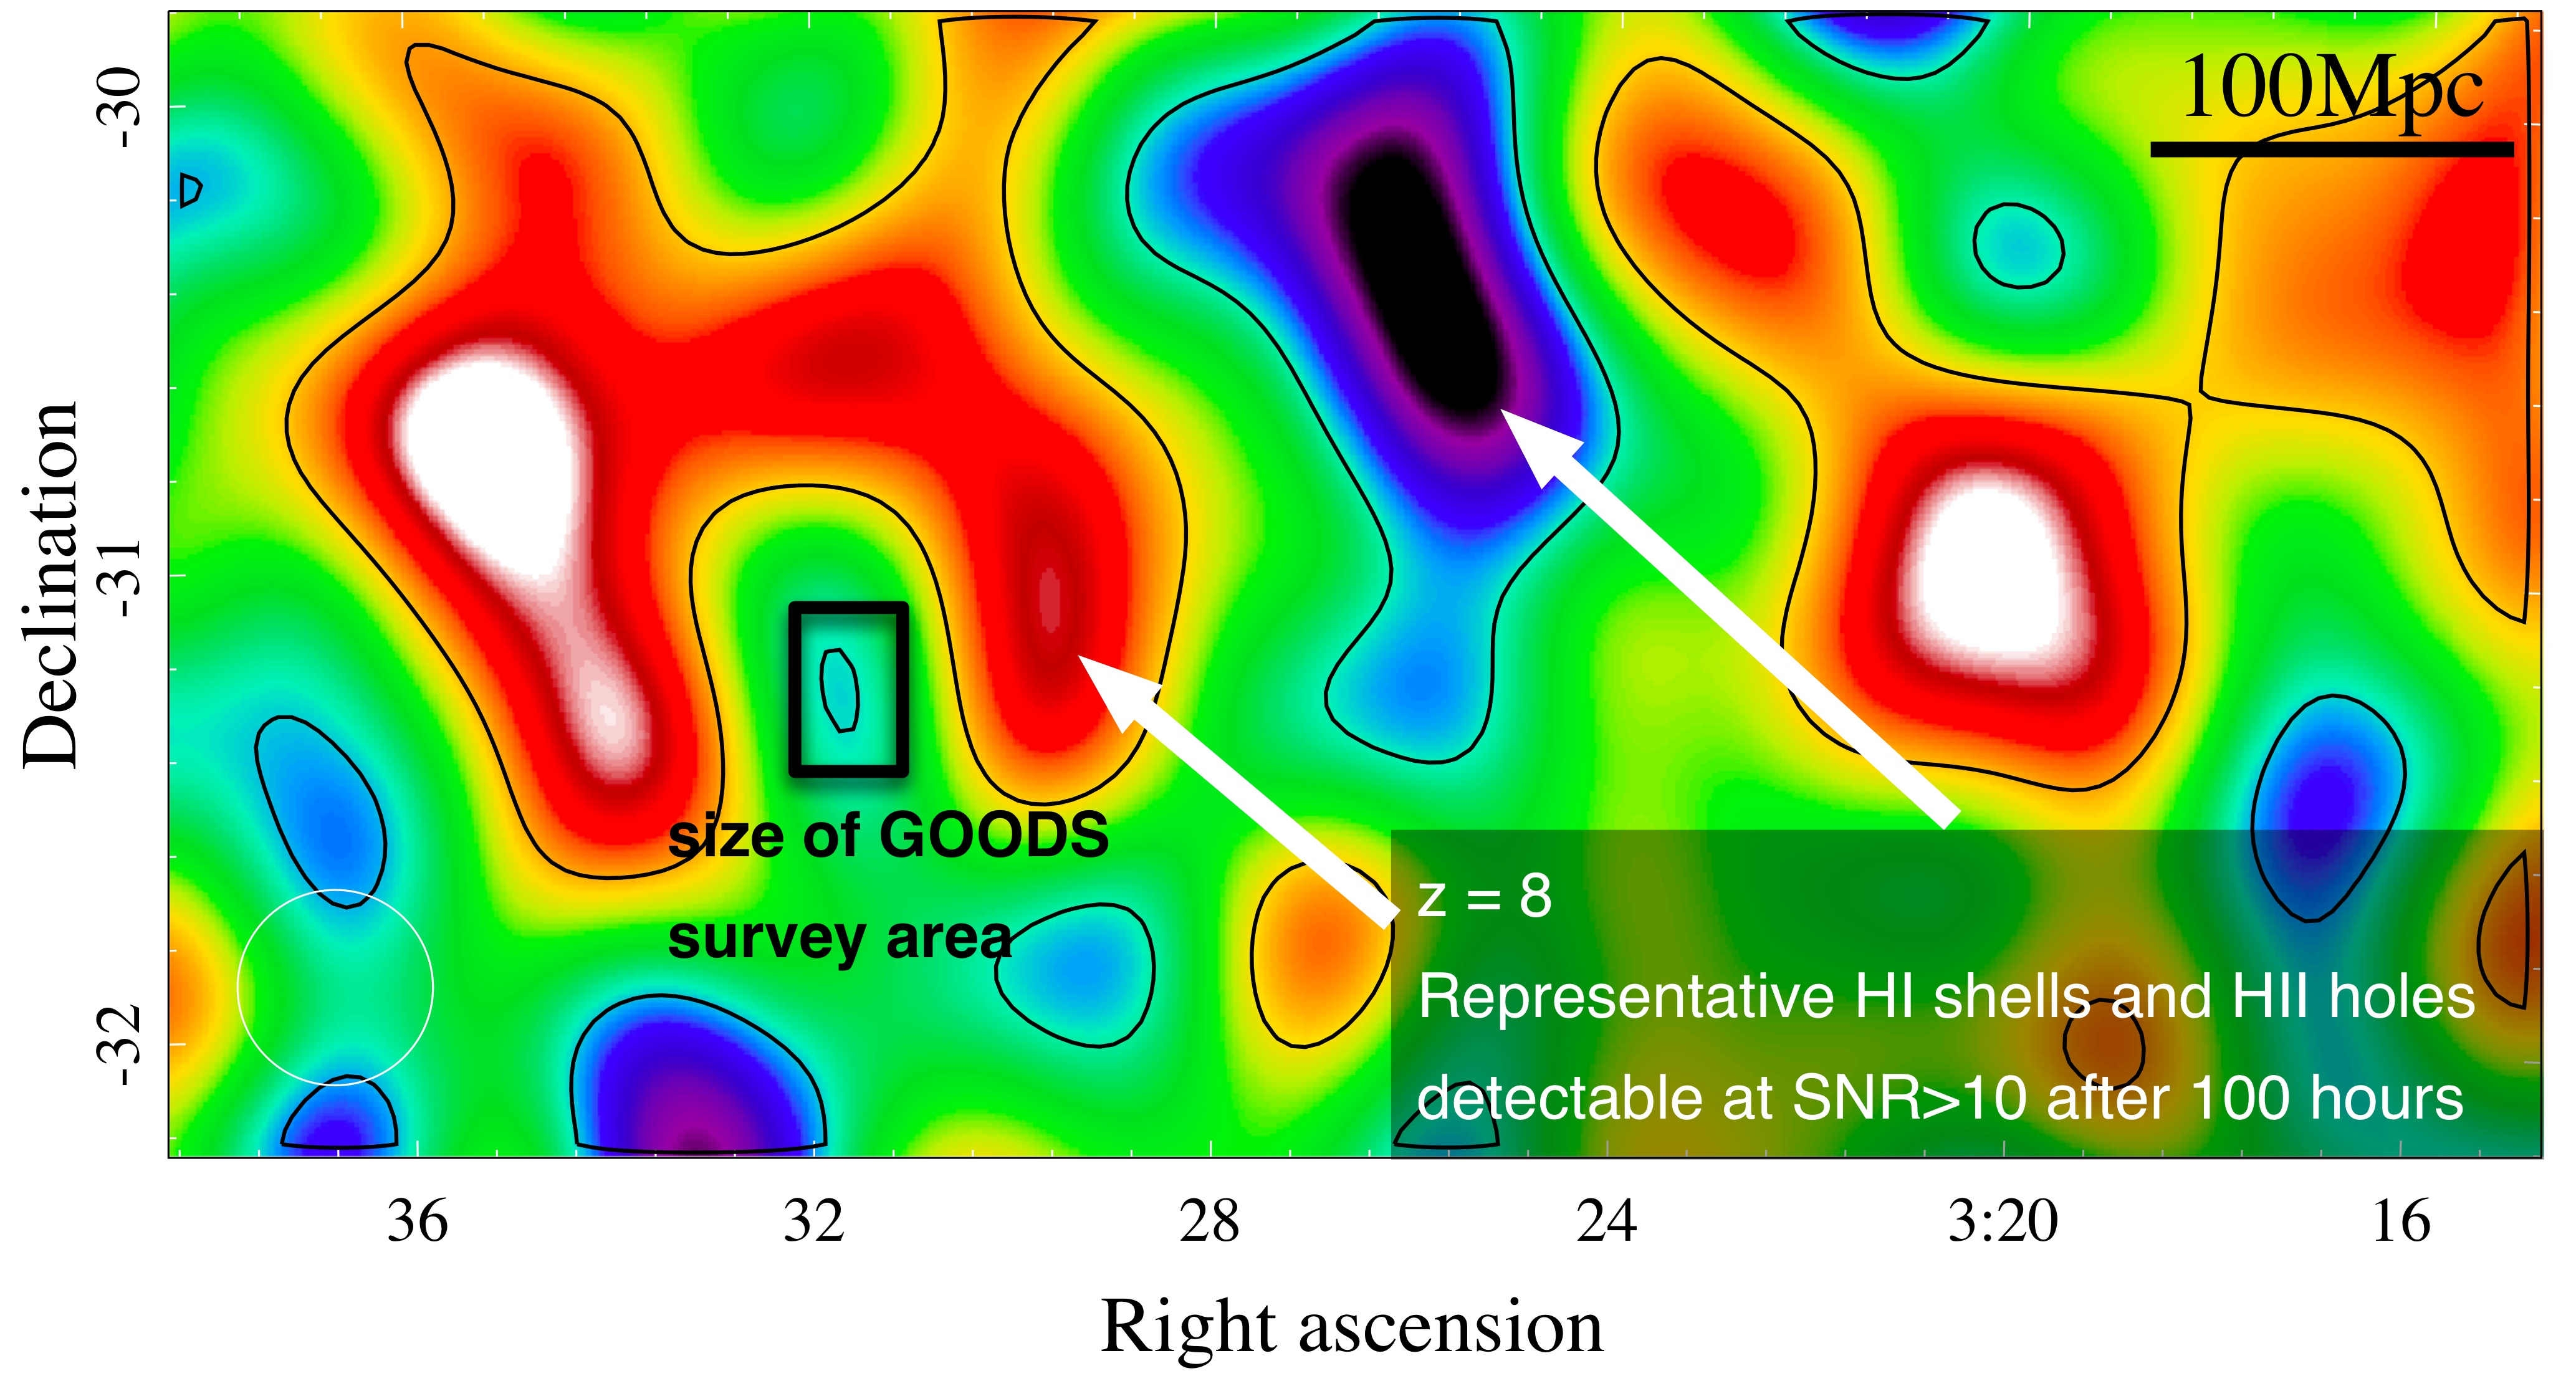
\includegraphics[height=2.5in]{plots/Imaging/HERA_331_z8_SNR_annotated.jpg}%HERA_331_z8_SNR_annotated.jpg}
\Caption{-0.15in}{0.9}{-0.1in}{\small
With sensitivity concentrated at the largest scales and a survey area of 2600 square degrees,
HERA-331 has the sensitivity to directly image HI during reionization.  Contours indicate 10$\sigma$ detections of
a simulated reionization field \citep{mcquinn_et_al2007} with a 100-hour observation.
%The regions detected on scales of $\sim$100~Mpc bracket the size scales probed by deep galaxy surveys.  At 150~MHz ($z=8.5$) the HERA field of view is 8\arcdeg.
%With a nearly completely sampled aperture over 300~m across, HERA will have the collecting area of Arecibo but with $500\times$ the survey speed. Each night, HERA drift scans 2600 square degrees.%, for a survey volume of 50`$Gpc^3$.
%The survey area includes the GOODS-South field \citep{dickinson_et_al2003} (denoted by the black rectangle).  As one of the best studied regions of sky, the GOODs-South survey volume includes 179 known objects above $z=7$, which represents $\sim45\%$ of all such objects over the entire sky.
}  \label{fig:imaging}
\end{figure}

%
%\begin{figure}[t]\centering
%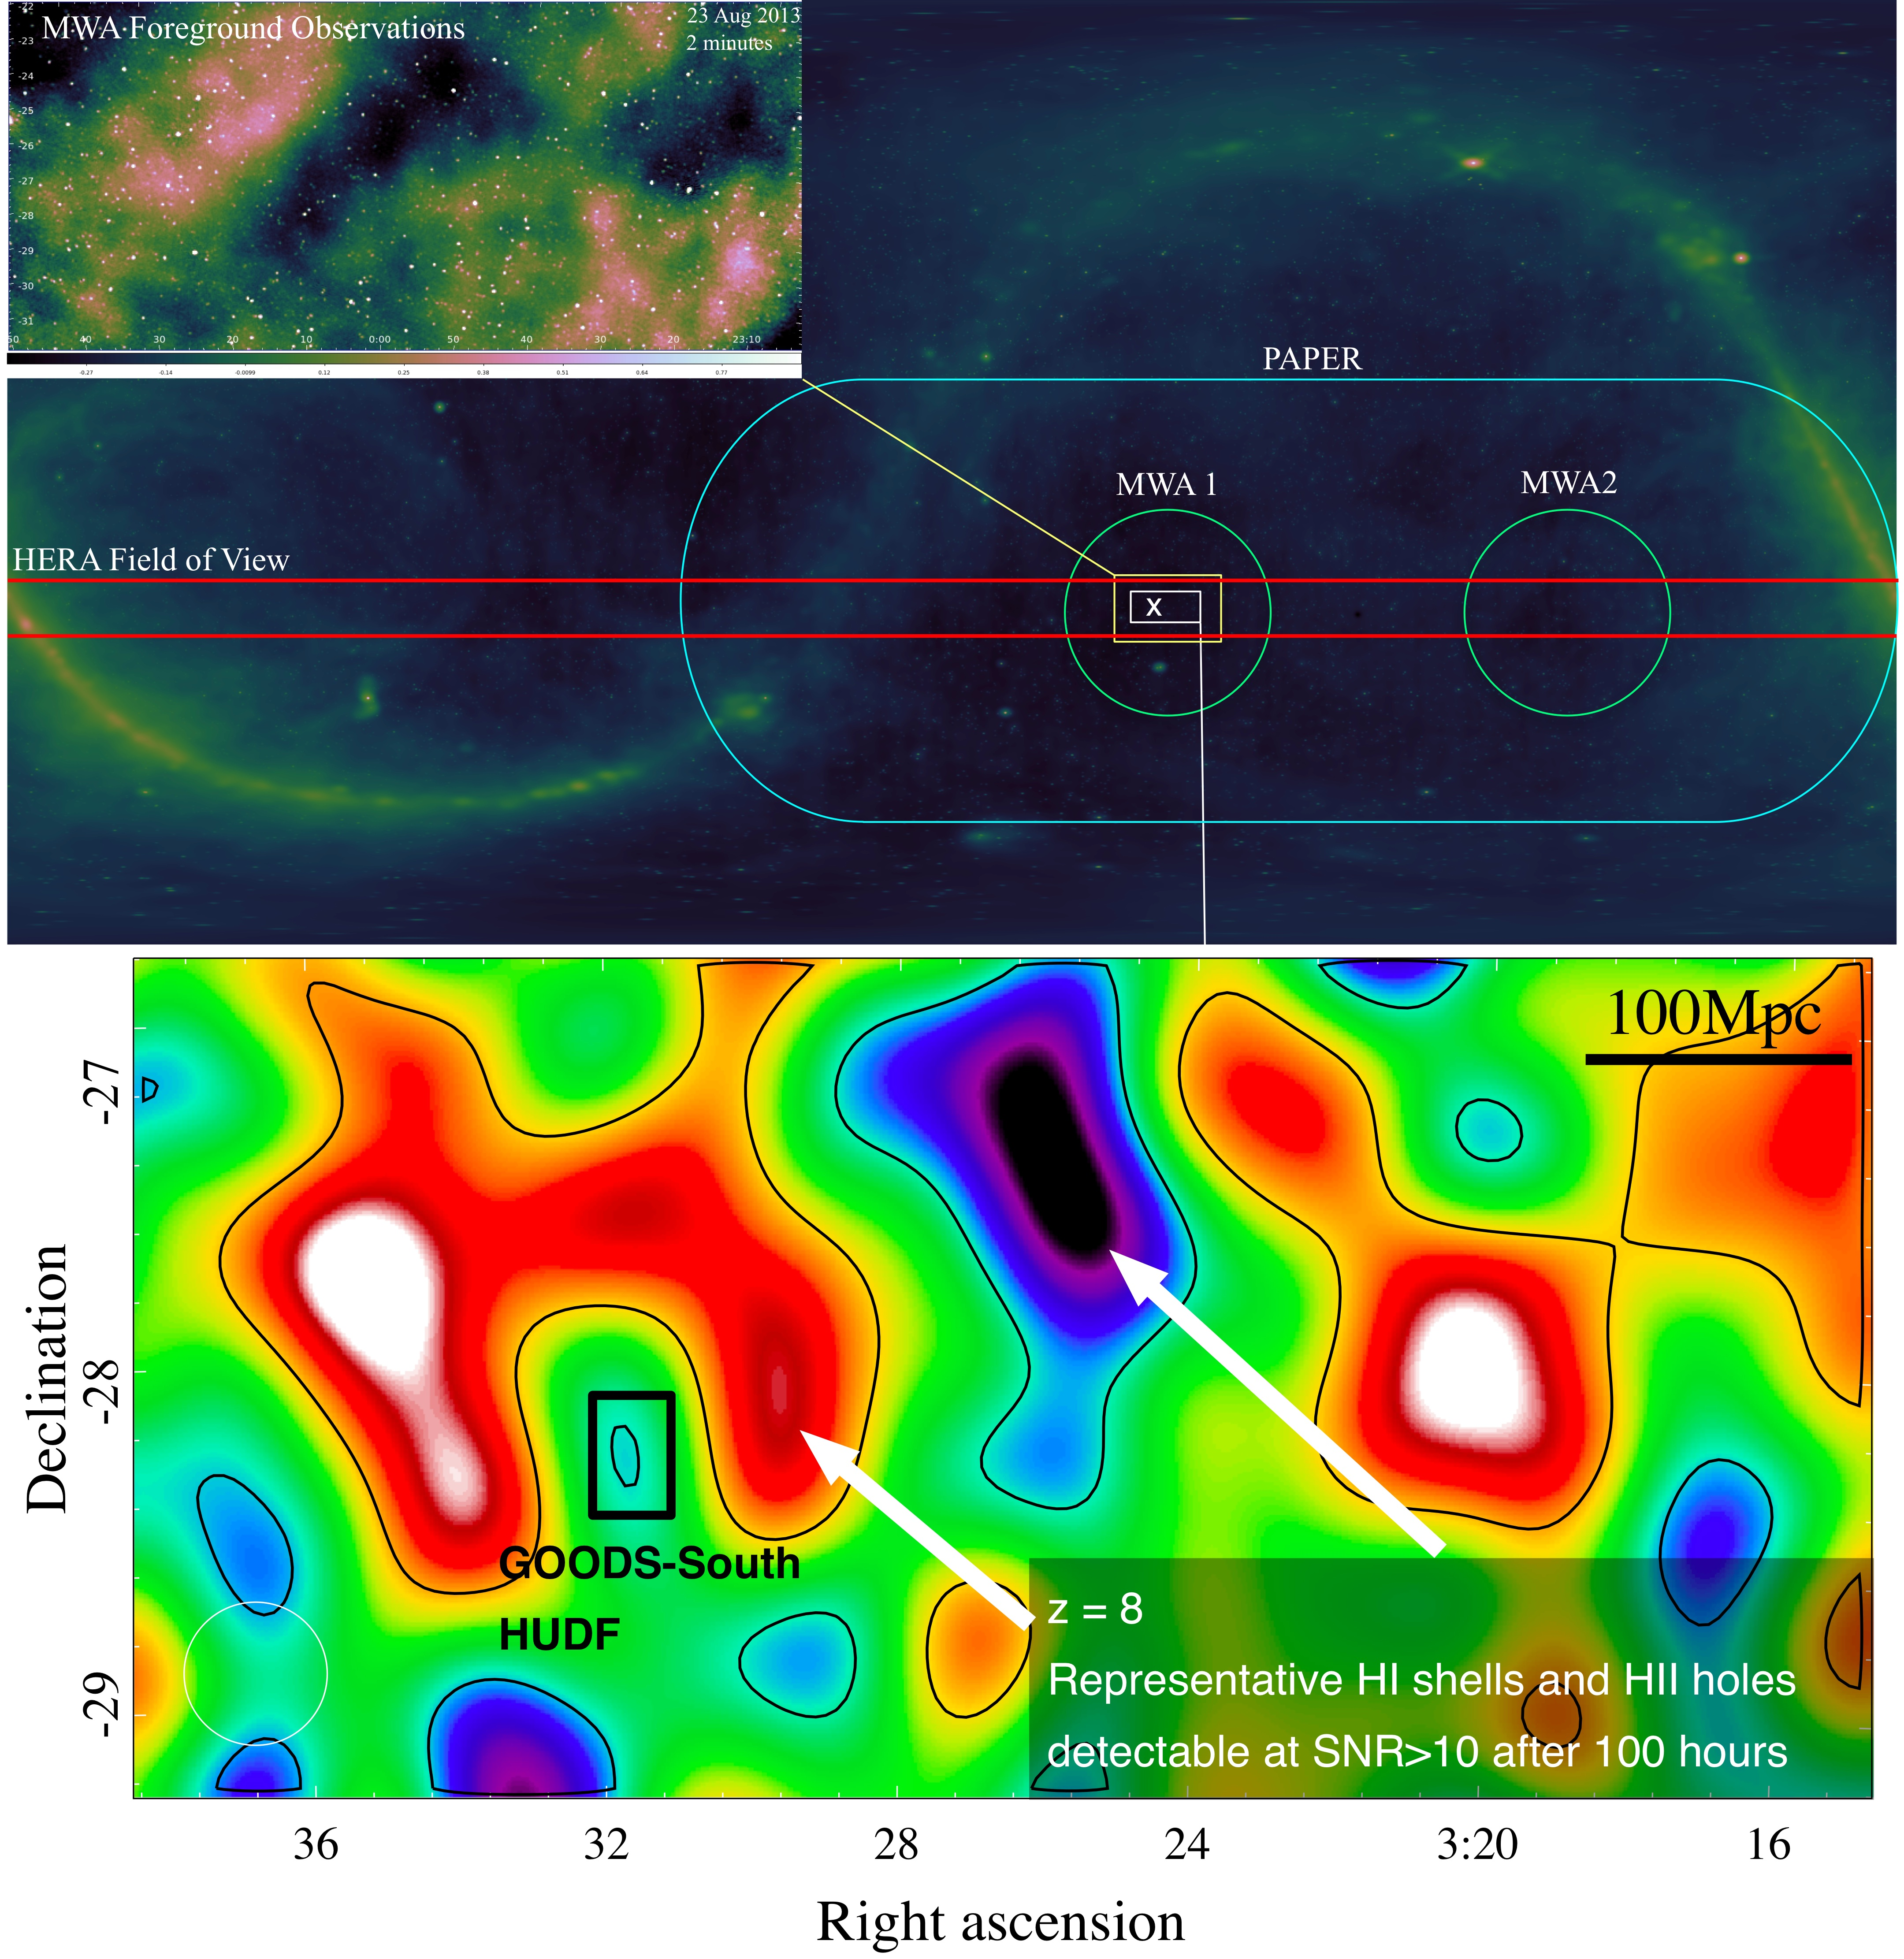
\includegraphics[width=\textwidth]{plots/Imaging/HERA_FoV_and_sim.jpg}%HERA_331_z8_SNR_annotated.jpg}
%\Caption{-0.2in}{0.9}{-0.2in}{\small
%With sensitivity highly concentrated at the largest scales, HERA is capable of directly imaging HI during reionization.  Shown here is the HERA ``stripe''.  At 150~MHz ($z=8.5$) the HERA field of view is 8\arcdeg.  With a nearly completely sampled aperture over 300~m across, HERA will have the collecting area of Arecibo but with 500x the survey speed. Each night it will drift scan 2600 square degrees for a survey volume of 50`$Gpc^3$.  The stripe includes the GOODS-South field \citep{dickinson_et_al2003}, one of the best studied regions of sky.  Shown here is a simulation of EoR emission \citep{mcquinn_et_al2007} as imaged by HERA with noise equivalent to 100 hours of observation.
%Contours enclose regions with signal to noise above 10.  The regions detected on scales of $\sim$100~Mpc are bracket the size scales probed by deep galaxy surveys (cf. the GOODs-South survey volume where 179 objects about $z=7$ have been detected, representing $\sim45\%$ of all such objects over the entire sky.)}  \label{fig:imaging}
%\end{figure}

%\subsubsection{Imaging as a probe of non-gaussianity}
%\emph{a) Imaging as a probe of non-Gaussianity and topology of reionization (Fig from Watkinson \& Pritchard)
%[Not sure if this belongs here, should discuss: b) Bayesian imaging (Figs from Paul Sutter).
%Perhaps a broader impact on the radio community too?]}
%% Morales, Tegmark

%\compress
%\subsubsection{Early IGM heating: the pre-reionization era}
%\emph{v. Approaching Dark ages (z=20 to 30): early Xray heating? other (Fig - Liu models)}
% Liu, Dillon, Hewitt
%\begin{figure}[t]\centering
%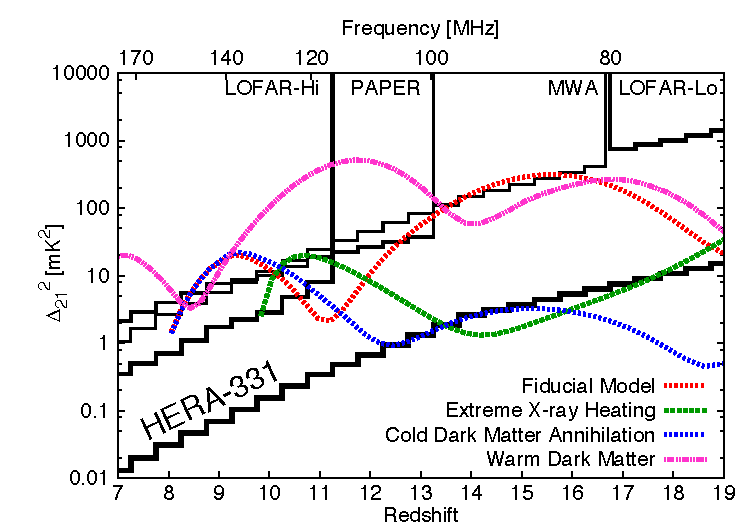
\includegraphics{plots/Xray/HERA_II_compare_kp1_whoriz_20pt.pdf}
%\Caption{-0.2in}{0.9}{-0.2in}{\small
%At low frequencies, HERA opens a window to
%pre-reionization physics at the end of the Dark Ages. Plotted are power spectrum amplitudes (at $k =
%0.15h$~Mpc$^{-1}$) for various IGM heating models \citep{mesinger_et_al2013},
%with predicted HERA sensitivities.
%% maybe merge this back in with x_i vs z figure in dark ages subsection
%}\label{fig:Xray} \end{figure}

{\bf Pre-Reionization Heating}. With high sensitivity throughout its observing
band, HERA pushes the redshift frontier of current-generation 21~cm instruments
to the pre-reionization era ($z \sim 20$).  This allows measuring an earlier
peak in the power spectrum that arises in standard theoretical models from an
era of IGM heating by X-rays from black hole binaries.  These scenarios allow a
wide range of possibilities for IGM heating, as shown in Figure
\ref{fig:x_i_vs_z} (see  \Mycitealt{mesinger_et_al2013}) with HERA's sensitivity
overlaid.  HERA's constraints in this epoch can determine the rate and density
of massive black hole formation in the early universe
\citep{pritchard_loeb2010}.  Alternate heating sources such as dark matter
annihilation cause easily identifiable contributions in some models, and at the
higher redshifts, exotic physics such as warm dark matter may also be
constrained.  HERA measurements are also be sensitive to velocity streaming
between baryonic matter and the dark matter halos, and its effect on early
structure formation and the onset of Ly$\alpha$ emission
\citep{visbal_et_al2012}.  HERA is uniquely poised to take advantage of
the pre-reionization era as an unparalleled testbed for both astrophysics and
cosmology.

%As seen in  Figure \ref{fig:x_i_vs_z}, the HERA 21~cm observations are sensitive to
%the rate and density of massive black holes formed in the
%early universe \citep{pritchard_loeb2010} via their X-ray emission (see Figure \ref{fig:x_i_vs_z}, right panel),
%how velocity streaming between baryonic
%matter and the dark matter halos affected early structure formation and the onset
%of Ly$\alpha$ emission \citep{visbal_et_al2012}, and will lay the groundwork for future
%efforts to explore how
%cosmological models can be improved via measurements of redshift-space distortions,
%artificial anisotropies introduced via the Alcock-Paczy\'inski effect, and
%gravitational lensing signals\citep{furlanetto_et_al2006}.

%vi. 21~cm forest: perhaps a paragraph on possibilities of small scale structure, if we can find radio galaxy? (Fig)
% Carilli, Furlanetto -- Forget it.  Too much explanation needed.

%\compress
%\subsubsection{Cross-correlation Science}
%vii. Cross-correlation science:

{\bf Cross-Correlations}. The ability of HERA to image enables an exciting range of cross-correlation science.
HERA HI images can reveal the large-scale reionization environment for pointed ALMA and JWST
observations and other deep near-IR surveys \citep{lidz_et_al2009}.
Knowing whether an observed galaxy is in a region that  was
previously reionized (center of large HII bubble), recently reionized (edge of HII bubble), or is forming from
pristine HI provides important contextual information on early galaxy formation and especially feedback.
HI images can also be cross-correlated with other diffuse
tracers of large scale structure, including intensity
mapping of molecular  CO \citep{lidz_et_al2011}, atomic CII \citep{gong_et_al2011}, and the HI Ly$\alpha$ \citep{silva_et_al2013} lines. These studies
trace the large scale galaxy distribution -- the sources of reionization — and cross-correlation 
with IGM images can break degeneracies within both data sets. Prototypes of such experiments
may be operating contemporaneously with HERA. Such probes have different systematics
compared to HERA, so cross-correlations provide clean measurements of the underlying signal.

%b. CMB pol
%Cross-correlations with the optical depth measurements \citep{sarkar_et_al2009,meerburg_et_al2013}
% CMB omitted because most studies look way too optimistic.  Probably not going to happen.  ACL
% c. CO/CII IM: optimistic or wrong timescale?
%e. Anscillary science with PAPER 128: transients, solar
% de Boer
%\clearpage

%  _                           
% | |   ___ ______ ___ _ _  ___
% | |__/ -_|_-<_-</ _ \ ' \(_-<
% |____\___/__/__/\___/_||_/__/

\compress
\section{Achievements Under Prior NSF Support} % this is a required section of the proposal
%\section{Why build HERA now, and the lessons from MWA \& PAPER}
%\subsection{Where we are right now: PAPER, MWA}  % 2 pages
%\section{Foregrounds \& Lessons Learned from PAPER and MWA} 

\begin{figure}[t]\centering
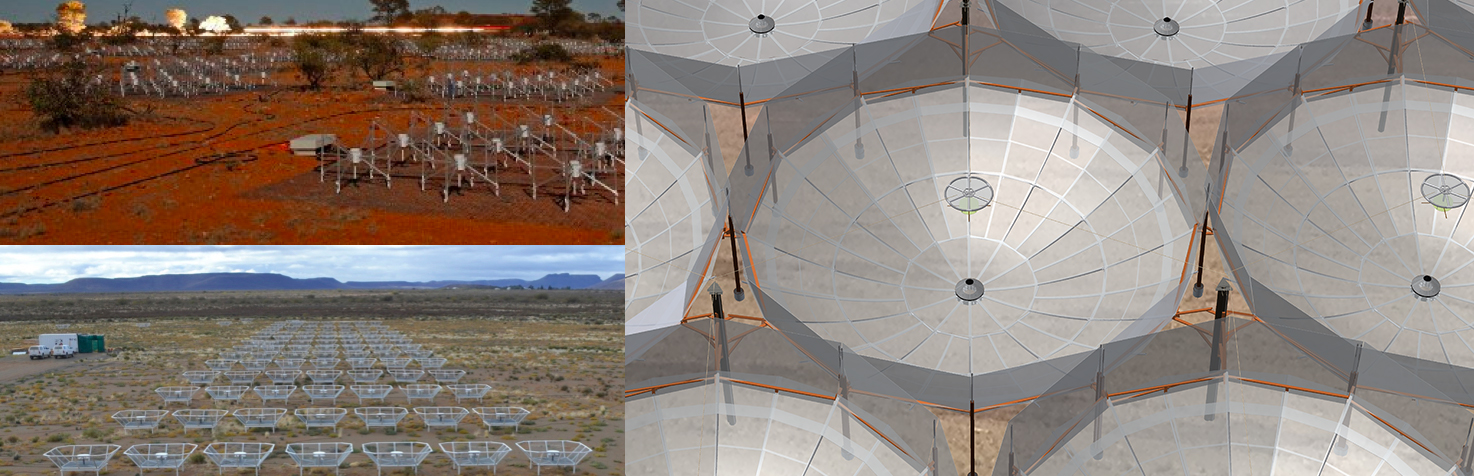
\includegraphics[width=6.5in]{plots/PAPER_and_MWA_and_HERA.jpg}
\Caption{-0.25in}{0.9}{-0.15in}{\small
The MWA (top left) and PAPER (bottom left) arrays, each currently deployed with 128 elements.
The 14-m HERA element (right) dramatically improves sensitivity while 
constraining the path length and amplitude of reflections to ensure that foreground
isolation is not substantially degraded.
%The core of HERA~331 consists of a redundant hexagonal array with
%outrigger antennas (not shown) for imaging and foreground mitigation.
}
\label{fig:hera_dish}
\end{figure}


The HERA project team consists of PIs and technical leaders from four NSF-funded projects targeting the 21~cm signal
at high redshifts:
\begin{itemize}[noitemsep,nolistsep]

\item{PAPER} (NSF grants \#1129258, \#0804508, \#0607838, and \#0505354) has followed a
staged development approach, maintaining a technical development array in Green Bank, WV, and
a science array in the Square Kilometre Array (SKA) radio quiet zone in the Karoo, South Africa.  Starting with a 16 element
array in 2009 in the Karoo, PAPER has doubled its size annually for four years running, culminating in the current
128 element array (Figure \ref{fig:hera_dish}; \Mycitealt{parsons_et_al2012a}).
%JCP: Parsons 2012a seems like an odd cite here... Parsons 2010? 
PAPER pioneered the use of redundant antenna configurations
for power-spectrum measurements, the use of drift-scanning elements,
a scalable correlator architecture,
and real-time 40-fold data compression based on delay/delay-rate filtering.
PAPER pioneered the delay-spectrum foreground avoidance technique \Mycitep{parsons_et_al2012b},
and applied it to observations (Fig. \ref{fig:eor_pspec}; \Mycitealt{parsons_et_al2013}).
The resulting power spectrum places the best upper
limit on reionization by almost two orders of magnitude in mK$^2$, and was used to show that the IGM must have
been heated prior to reionization --- presumably by emission from high-mass X-ray binaries.

\item{The MWA} (NSF grants \#0457585, \#082132, \#1109257), 
located at the future SKA-low site
in Western Australia, was developed as a large international collaboration.  It consists
of 128 digitally steerable antenna tiles (Fig. \ref{fig:hera_dish}, upper left;
\citealt{tingay_et_al2013}), arranged in an imaging configuration, and operating from 80 to 300 MHz.
%The MWA's hardware performance \citep{bowman_et_al2007a}, calibration pipeline
%\citep{mitchell_et_al2008}, and foreground subtraction strategy \citep{morales_et_al2006a}
%are well documented. 
The US MWA team is a world leader in the application of image-based modeling techniques 
(Fig. \ref{fig:twoFGViews}, left) to
foreground subtraction (e.g. \Mycitealt{hazelton_et_al2013,morales_et_al2006a}). %for enlarging the EoR window for power spectral studies, 
Recent MWA observations have
demonstrated the subtraction of foregrounds to the thermal noise limit in regions dominated by systematics using
delay-spectrum analysis techniques (Fig. \ref{fig:twoFGViews}, right).
%and enabling imaging of reionization (Figure
%\ref{fig:eor_pspec}). The resulting analysis is more complex than the
%delay-spectrum approach (e.g.\ \citealt{hazelton_et_al2013}) but 
%naturally
Such techniques potentially
expand the number of modes available to HERA for measuring the 21~cm reionization signal,
and can suppress polarized foregrounds that may enter delay-spectrum measurments near
the level of the reionization signal \Mycitep{moore_et_al2013}. 
%comparison with observations at other bands. 

\item{MITEoR} (NSF grants \#1105835, \#0908848) is 64-element array 
examining novel cross-correlation and calibration techniques for 21~cm reionization experiments.
While spatial-FFT cross-correlation
techniques remain under development, MITEoR brings critical expertise in redundancy-based calibration
and quadratic power-spectrum estimation techniques.

\item{LEDA} (NSF grant \#1106045) is a 256-element array targeting the
global 21~cm reionization signal.  Werthimer and Greenhill collaboratively 
pioneered the application of graphics processing units (GPUs) in digital correlators.
This technology was adopted in recent PAPER deployments, and is applied to HERA's correlator
and data-compression systems.

\end{itemize}

\noindent
Other projects invoving HERA team members that have undertaken significant hardware development and
completed major deployments include the EDGES experiment (NSF grants \#1207761, \#0905990),
the Center for Astronomy Signal Processing and Electronics Research (CASPER; NSF grant \#0906040), the Advanced Multibeam
Spectrometer for the GBT (NSF grant \#1006509), and numerous other efforts.  On the theory side, 
%\noindent {\bf Furlanetto:} Furlanetto held 
``Theoretical Models of Helium Reionization" (NSF grant \#0829737, \#0607470) 
%(an institutional transfer of AST-0607470; these two grants provide \$358,486 over the period 9/1/2006--8/31/2009).  This grant led to 13 journal articles, published over the period 2007--2010, with several more in the years since. The primary broader impact were training a graduate student, Keri Dixon, 
created and publicly distributed the semi-numeric reionization code, DexM.  The broader impacts of these
efforts are discussed in \S\ref{sec:other_broader}.

These projects have a strong publication records of ground-breaking research in peer-reviewed literature, and
bring to HERA mature hardware designs, software pipelines, and powerful scientific and analysis frameworks.
HERA's leadership also brings substantial experience
collaborating internationally, managing the design, development, testing, and integration of complex systems,
adhering to project timelines and budgets, and setting incremental development and deployment plans that
ensure that progress is made on a predictable schedule, with time to adapt to contingencies.

\compress
\subsection{Lessons for HERA}
\label{sec:Lessons}

\begin{figure}[t]\centering
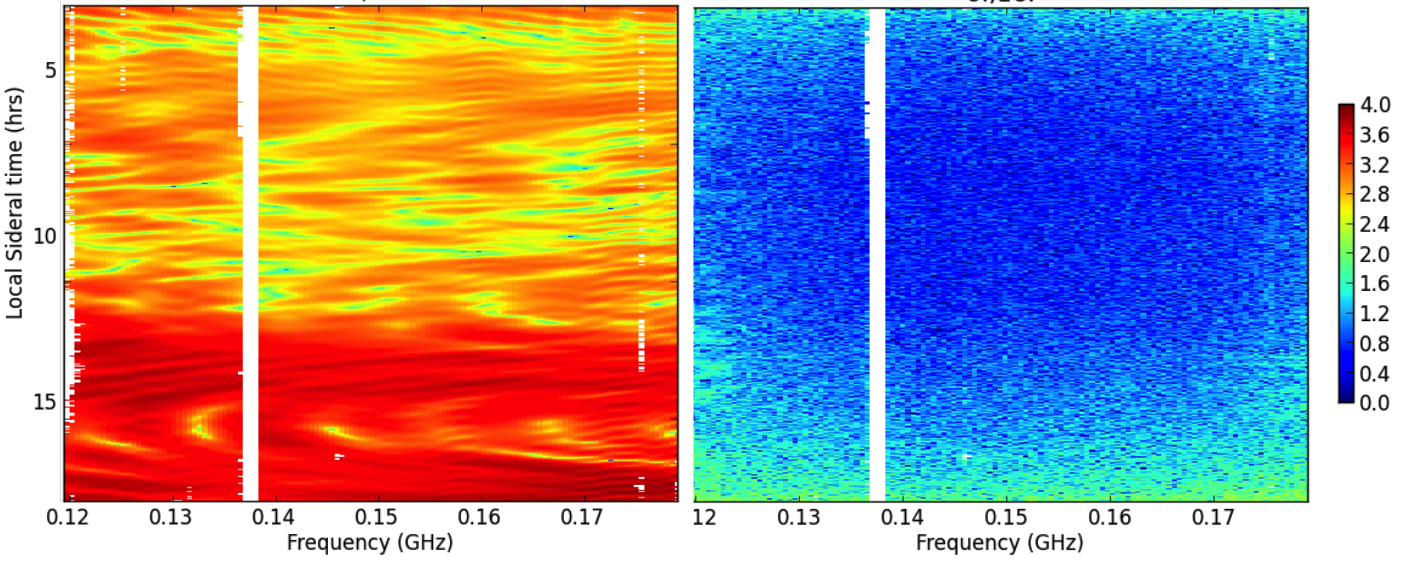
\includegraphics[width=6in]{plots/waterfall_filtered.png}
\Caption{-0.15in}{0.9}{-0.15in}{\small 
Waterfall plots illustrating PAPER visibilities
measured on a 30-m baseline before (left) and after (right) the application of a 
delay filter that removes forground emission within the wedge.  Color scale indicates amplitude in $\log_{10}({\rm Jy})$.
This filter suppresses
foreground systematics by $>4$ orders of magnitude, leaving residuals demonstrably noise-dominated while preserving the reionization signal.
}\label{fig:waterfall} \end{figure}


The key challenge of 21~cm reionization experiments is 
balancing the collecting area needed to detect the faint reionization signal
with the precision needed to suppress
foregrounds that are $\sim$5 orders of magnitude brighter \citep{deoliveira2008}.
Previously, it was assumed that careful calibration and image-based model subtraction would be the keys to overcoming these foregrounds.
While such efforts are being actively pursued, and are likely to be important to the field in the future,
it has become clear that the community underestimated the challenges associated with this approach.
The major breakthrough for 21~cm reionization experiments --- what enables us to propose HERA now --- is 
the discovery of how 
instrumentation and analysis can instead exploit the 
spectral smoothness of foregrounds 
to open up a window for accessing the reionization signal. 
%These advances have been pioneered by the MWA and PAPER teams \citep{morales_et_al2012,parsons_et_al2012b,vedantham_2012,Datta_2010,hazelton_et_al2013,pober_et_al2013,parsons_et_al2013,dillon_et_al2013b}, and enable us to design a targeted HERA instrument that can reveal the details of reionization (Figure \ref{fig:x_i_vs_z}) and image the largest structures (Figure \ref{fig:imaging}).
As illustrated in Figure \ref{fig:waterfall}, these advances have been used to suppress foreground emission by at least 4
orders of magnitude in PAPER observations,
with results that begin ruling out certain reionization scenarios
\Mycitep{parsons_et_al2013}.

%Observations for 21~cm cosmology experiments are best understood in Fourier space.  
For redshifted (21~cm) line emission, each observing frequency maps to
a line-of-sight distance.  Hence, measurements as a function of frequency and angle 
to enable 21~cm reionization experiments to map a cosmological volume $\{x,y,z\}$ in
comoving Mpc.  For power-spectrum measurements, this observed volume is Fourier transformed into a 
wavenumber cube $\k\equiv\{k_{x}, k_{y}, k_{z}\}$, where 
$\kperp\equiv\{k_{x},k_{y}\}$ represents angular Fourier modes that are directly
related to the $(u,v)$ modes sampled by baselines of an interferometer, and $\kpar\equiv k_{z}$ is
a line-of-sight wavenumber.
%Interferometric measurements are of the angular Fourier modes in many
%frequency channels (visibilities), so in the absence of widefield effects only
%a Fourier transform in the frequency direction and a coordinate mapping is
%needed to obtain the 3D $\{k_{x}, k_{y}, k_{z}\}$ measurements
%\citep{morales_hewitt2004}.) 
The expected statistical isotropy of the signal allows measurements in $k$-space to be
squared and averaged in shells to produce the spherical power spectrum
shown in Figure \ref{fig:eor_pspec}.

\begin{figure}[t] \centering
%in]{plots/MWApretty.png}
%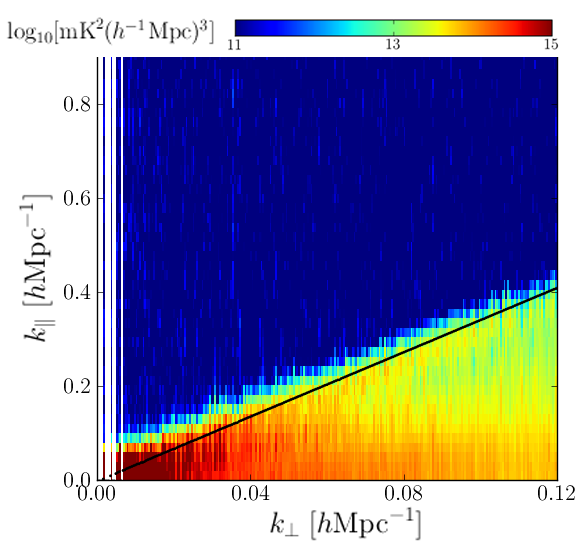
\includegraphics[height=2.02in]{plots/wedge_tall_wide.png} 
%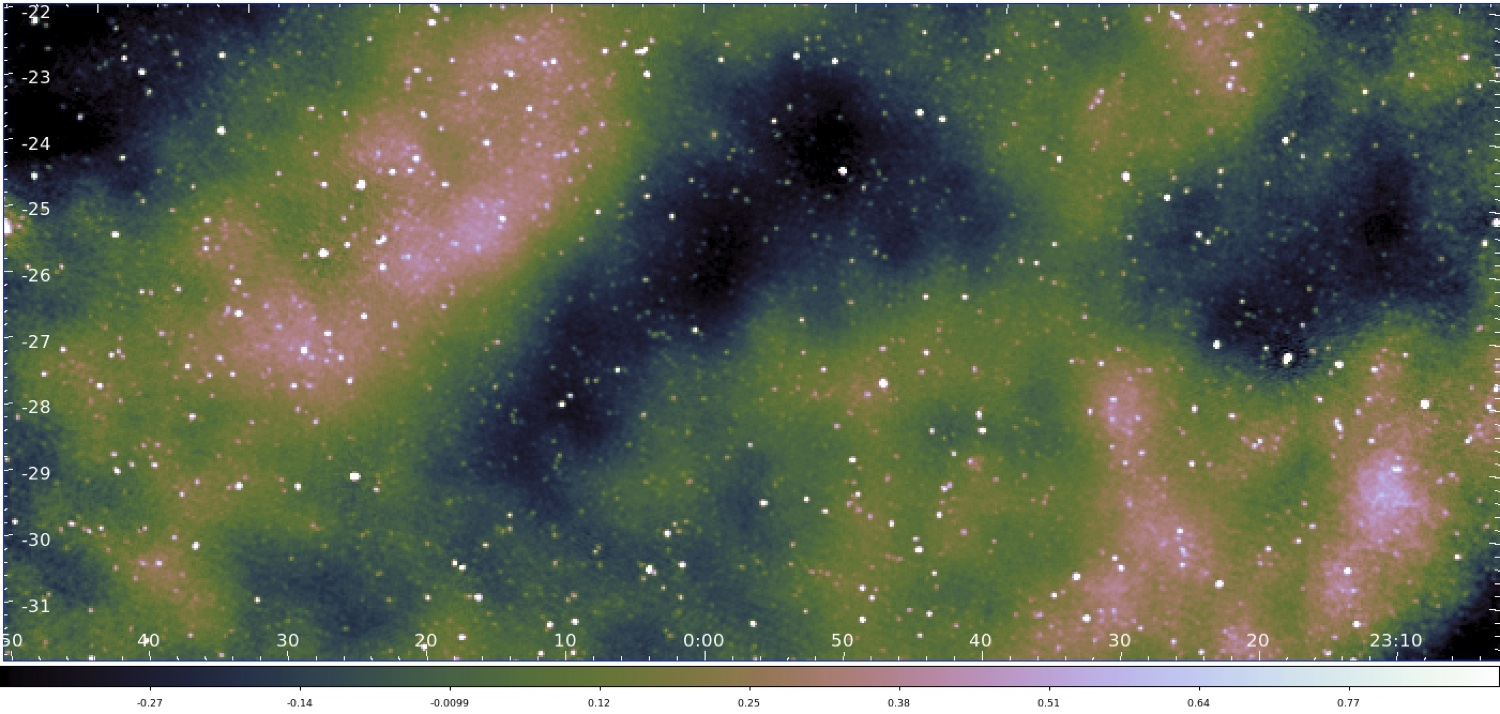
\includegraphics[height=2.02in]{plots/Foregrounds/MWA_EoR0_2min.jpg}
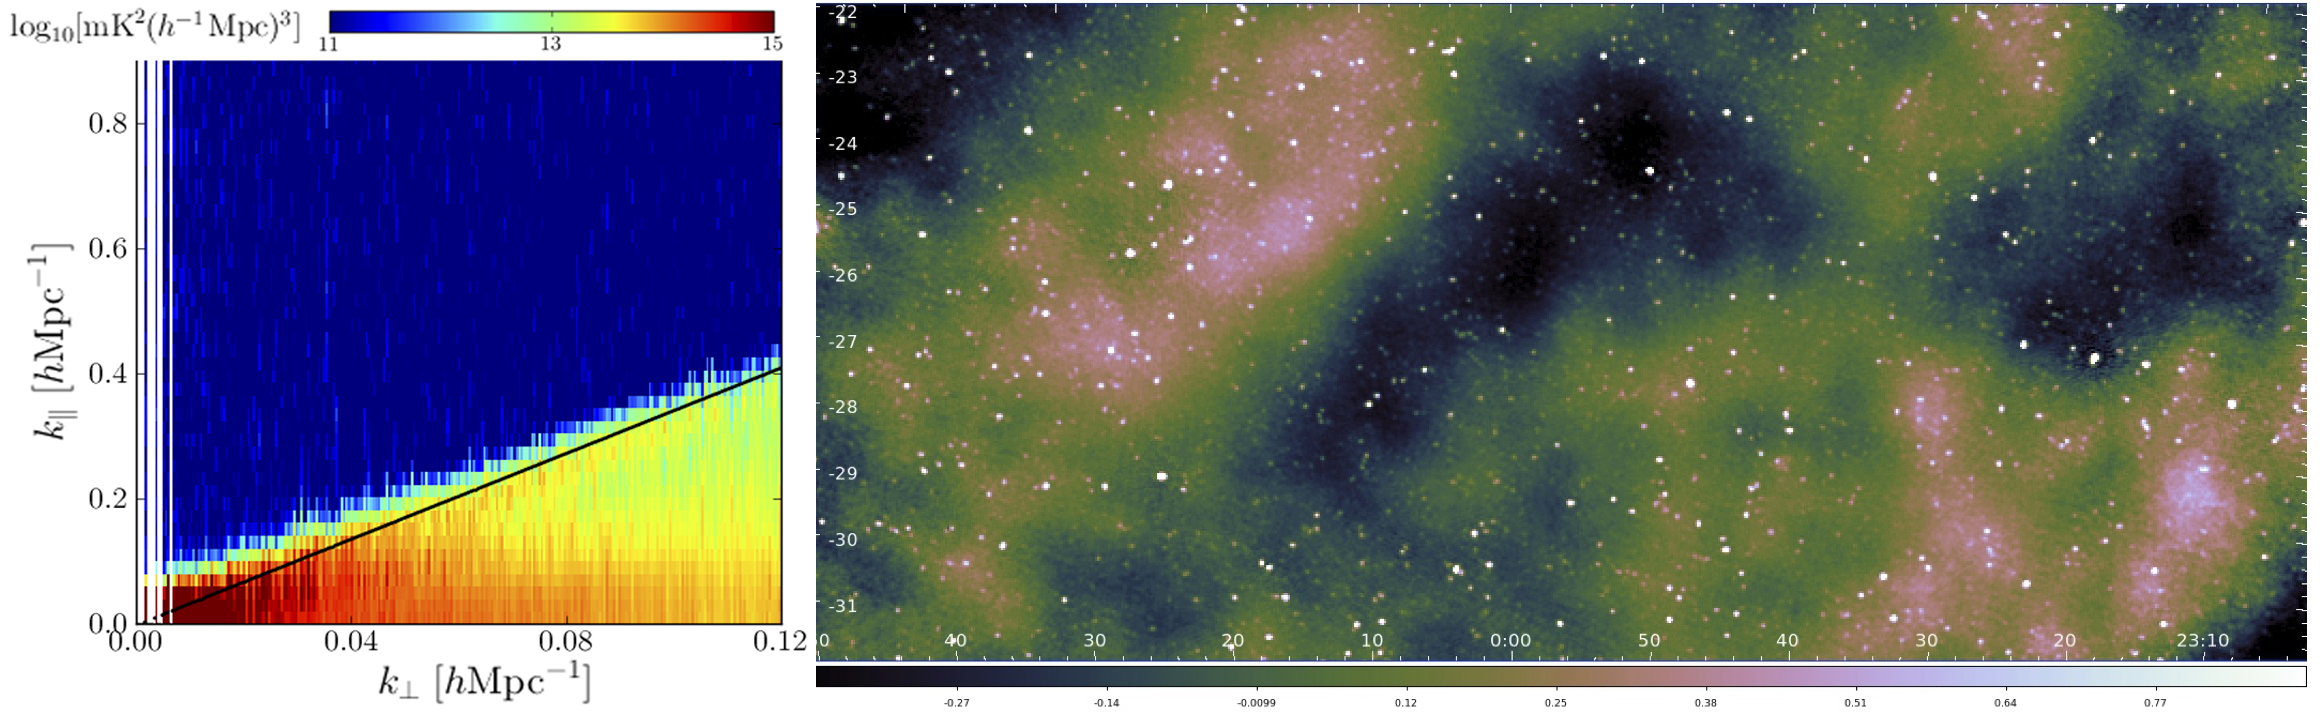
\includegraphics[height=2in]{plots/Foregrounds/MWA_wedge_consolidated.jpg}
\Caption{-0.3in}{0.9}{-0.15in}{\small Left:
PAPER observations \citep{pober_et_al2013} show foreground contamination 
in line-of-sight $\kpar$ vs.\ angular $\kperp$ to be
confined to a bright wedge,
leaving other modes thermal-noise limited.
% ARP: this isn't a bad sentence below, but can maybe leave it to the text to describe?
%The width of the wedge derives both from an instrument-independent component 
%(solid black line) and an additional component relating to the inherent spectral smoothness
%of both the foregrounds and the instrument response.
Right:
An $\sim10^{\circ} \times 25^{\circ}$ image of foregrounds by the MWA illustrates
methods that provide key capabilities for reducing
polarization leakage and foreground systematics within the wedge for HERA observations.  
}\label{fig:twoFGViews} \end{figure}


%Imaging-based approaches combine baseline measurements to
%invert the $\kpar\Leftrightarrow(u,v)$ modes natively
%sampled by an interferometer, and then aim to calibrate out the inherent chromaticity of an
%interferometer's $(u,v)$-sampling to enable the accurate subtraction of foreground models.
Rather than inverting interferometric measurements to make images,
a powerful new approach has been developed and tested by the PAPER
and MWA teams that instead directly Fourier transforms each baseline separately along the frequency axis,
effectively producing a wavenumber cube while still handling inteferometric
chromaticity on a per-baseline basis.  Because of the way smooth-spectrum foregrounds
interact with baselines of different lengths, this flexibility to handle
baselines separately is critical.
Through a concerted theoretical and observational campaign by PAPER and the MWA
(\Mycitealt{morales_et_al2012,parsons_et_al2012b};\citealt{vedantham_2012};\Mycitealt{Datta_2010,hazelton_et_al2013,pober_et_al2013,parsons_et_al2013,dillon_et_al2013b}),
we now understand that foreground contamination is confined to a `wedge' in
$\kpar$ vs.\ $\kperp$, as demonstrated by the PAPER observations in 
Figure \ref{fig:twoFGViews}. Because the $\kpar$ direction (obtained by
Fourier-transforming along the frequency axis) is effectively an ``inverse frequency'' (e.g. time delay),
the form of this wedge can be understood analytically as arising from the relative delay between sky signals
entering each antenna in an interferometric baseline from different directions.
(Faraday-rotated emission from extragalactic sources may introduce additional foreground emission outside the wedge \Mycitep{moore_et_al2013};
we discuss plans for mitigating polarization leakage and removing this source
of contamination in the Analysis/Science Risk section of the Project Managment Plan.)

Our new understanding of the foreground wedge has two powerful consequences.
Firstly, as illustrated in Figure \ref{fig:waterfall}, the foreground wedge can
removed with a baseline-dependent filter that removes emission within a well-defined range of spectral smoothness.
This filter directly suppresses foregrounds by at least
4 orders of magnitude,  
and leaves the region above the wedge free from 
foreground emission --- a window through which we can observe the reionization signal.
Secondly, by understanding signal delay as the mechanism that gives rise to the wedge,
it is now possible, for the first time, to map foreground removal requirements 
to the precise instrumental characteristics that are required.  The most direct instrumental
constraint comes from that fact that, to access $\k$-modes in the range $0.1<k<0.2h\ {\rm Mpc}^{-1}$
where 21~cm reionization experiments can be most sensitive, {\bf the signal delay between antennas
contributing to this measurement cannot exceed 120 ns}.  As discussed in \S\ref{sec:design}, this
constraint can (and must) be incorporated into the fundamental design of any future 21~cm reionization instrument.
%JCP: is this the signal delay between antennas or within an antenna???

%%MM: a figure showing results from both arrays would be really powerful here.
%This wedge is the result of
%the smooth spectrum foregrounds 
%% SF: I would make this more obvious.  I recommend replacing this sentence with something like (with my naive understanding): "This sharp division occurs because foregrounds have smooth spectra (which cause the sources to manifest at small $\kpar$), some of which is projected into the transverse direction ($\kperp$) through the instrument's well-understood chromatic properties."
%(low $\kpar$) interacting with the inherent
%chromaticity of an interferometer. 
%This leaves the region above the wedge free from 
%foreground emission---a window through which we can observe the EoR. 
%As demonstrated in the right-hand panel of Figure \ref{fig:waterfall}, removal of the foreground wedge 
%directly suppresses foregrounds by at least 4 orders of magnitude.
%We now understand the source of the EoR window, how we can increase the 21~cm signal region, and have seen the window in observations with both PAPER and the MWA \citep{pober_et_al2013,dillon_et_al2013b}.
%
%%The time is now ripe for an experiment that builds from the technical heritage
%%of PAPER, the MWA, MITEoR, and LEDA, and incorporates into the design of the
%%instrument new insights relating to the interplay of sensitivity and the
%%foreground wedge.  HERA's new 14-m dish, whose design is motivated by the core
%%tenets delay-spectrum foreground avoidance, is foundational to this effort.
%%These elements, arranged redundantly in a compact hexagonal grid, enable both the
%%delay-spectrum foreground avoidance and calibration from PAPER (redundant
%%baselines, proven performance, low risk) and the foreground subtraction and
%%imaging from the MWA (filled $uv$~coverage, higher sensitivity and immunity to
%%polarized foregrounds).
%
%%HERA's signal path includes the dipole and balun from PAPER, with refinements
%%to broaden the spectral response to lower frequencies and optimally illuminate
%%the parabolic reflector.  Digital nodes near the antennas limit cable
%%reflections, and incorporate design elements of the MWA, PAPER's CASPER-based
%%digitization and filtering, and the hybrid FPGA/GPU correlator architecture
%%used by PAPER, the MWA, and LEDA.  HERA's software includes the Monitor \&
%%Control and meta-data systems from the MWA
%%redundant calibration pipelines from MITEoR and PAPER, delay-spectrum analysis from PAPER, Fast
%%Holographic Deconvolution imaging software
%%\citep{sullivan_et_al2012_trunc} and the imaging power spectrum
%%software from the MWA, and the backend computing infrastructure from PAPER.


%Observations with PAPER and the MWA have confirmed the presence of the EoR Window
%\citep{pober_et_al2013,dillon_et_al2013b}, and recent PAPER observations
%have measured the foreground suppression within it
%to be at least 4 orders of magnitude 
%(8 in mK$^2$;
%\citealt{parsons_et_al2013}).
%This is a major advance---we can
%suppress foregrounds and we understand the instrumental and analysis
%characteristics needed to perform the EoR measurement.
%
%Understanding the origin of the EoR Window has enabled us to improve our
%instrumentation and analysis 
%tools to precisely measure the 21~cm
%signal. HERA's antennas (see \S \ref{PDsec}) are optimized 
%to yield $\sim$20
%times the sensitivity per element (relative to PAPER) without substantially degrading
%foreground isolation,
%and we have developed new imaging and
%analysis techniques to suppress polarized source contamination to below the EoR
%signal within the window \citep{bernardi_2013_trunc,moore_et_al2013}.
%Together, these advances provide the necessary foreground suppression and
%a game-changing level of sensitivity at a fraction of the
%cost anticipated in the HERA roadmap.

%  possibly pull some of the sentences below for HERA Lessons section above.

%The HERA collaboration has made significant progress on multiple approaches in dealing with
%foregrounds.
%Based on a ``delay-spectrum'' understanding of
%the mechanism for how instrumental responses modulate foregrounds on
%spectral scales of cosmological interest \citep{parsons_et_al2012b},
%PAPER has optimized its instrument to focus on regions in Fourier
%space that have weak coupling to foregrounds caused by the
%interferometer.  These regions are determined both by chromatic
%instrumental responses and by the inherent frequency structure of the
%foregrounds.  An `EoR window' has been identified in the Fourier
%(wavenumber) space of spectral and angular power spectra that is
%inherently free of continuum emission, without explicit continuum
%subtraction in either the image or spectral domain \citep{pober_et_al2013,morales_et_al2012,Datta_2010}
%This window allows for continuum
%`avoidance' rather than subtraction. Observations based on this new
%approach have already demonstrated that the extremely stringent level
%of foreground suppression needed to access the 21~cm signal is largely
%in hand (as shown in Figure \ref{fig:pk_k3pk}), with upper limits
%that are beginning to rule out cold reionization scenarios \citep{parsons_et_al2013}.



%i. describe arrays, state design driven by new understandings as delineated below (Fig)
% ARP: check, above % Parsons, Bowman

%ii. Using new techniqes, current best limits  (Fig)
% ARP: check, above % Parsons, Morales

%iii. what will happen in next 2 years: hopefully detection, but no more

%iv. LOFAR/MWA/PAPER 
% Carilli
% ARP: I think paragraph below should really emphasize concrete limitations of 
% current experiments, and describe how HERA blows this wide open
%Three reionization path-finder array experiments are currently
%operational: LOFAR, MWA and PAPER. All three are designed to have the
%sensitivity to make the first statistical detection of the neutral
%IGM. However, the HI line experiment is very challenging due to
%foreground continuum emission some four orders of magnitude brighter
%than the expected line signal.  The three experiments offer very
%significant complementarity, with different intrinsic systematics and
%different approaches to foreground mitigation. We emphasize that, for
%such an important discovery, multiple approaches are critical in order
%to check and verify any claimed (likely low S/N) detection amidst the
%substantial systematic uncertainties. The first detection of
%the neutral IGM is not the end of reionization studies, just the 
%beginning. Recall that some four decades separated the first detection
%of the CMB from the first statistical characterization. 
%
%
%iv. HERA II: 'gauranteed' detection, full characterization, dark ages, imaging
%% Aguirre
%
%v. Move 'analysis' stuff here?

%%%MM:  I think the Challenges have been largely subsumed into the above section, at the level of detail we want to put in a proposal, so I've commented out this section. Just a thought.

%\section{Challenges} % 2 pages
%
%\subsection{Foregrounds}  % 1.5pages
%% Parsons, Morales
%
%
%i. relative intensities (Fig: Continuum from MWA)
%
%ii. Details on Delay Spectrum approach
%
%a. key: 3D k-space: show wedge and discuss. chromatic sidelobes with characteristic freq scale 
%set by baseline length
%
%b. analysis focuses on line-of-sight PS dimension
%
%c. work in EoR window.  different window levels, depending on effective horizon
%
%d. drives design to redundant array: helps calibration, add spectra coherently
%
%e. dictates geometry of antenna elements and other RF stuff. avoid standing waves of given length. 
%
%f. area: drives sensitivity as used in section 2
%
%g. some words about why compact, hex array 
%
%\subsection{Other Challenges} % 0.5 pages
%
%i. Interference: Karoo RFI plots  FIG 
%% Jacobs
%
%i. Polarization 
%% Moore, Aguirre
%% ARP: I'm worried about this section.  In my mind, this is the one risk we
%% haven't truly retired yet.  We need to tread very carefuly if we bring this
%% up in depth.
%
%D. Ionosphere: 
%
%i. short baselines and narrowish FoV
%
%ii. direction dependent gains?



%  ___         _           
% |   \ ___ __(_)__ _ _ _  
% | |) / -_|_-< / _` | ' \ 
% |___/\___/__/_\__, |_||_|
%               |___/      

\compress
\section{HERA Project Design} % 8 pages
\label{sec:design}

% the proposal would be more convincing as an
% "experiment" if there were more of a flow from a specific science goal, down to
% technical requirements, down to your implementation.  This would boost
% reviewer's confidence that you will achieve a specific stunning science result
% if the project is funded.  And I think it will save you a few pages of text
% because there is a lot of repetition about things like avoiding reflections
% which could be eliminated if explained clearly at the outset.  And some
% important things are never justified, like the area of the survey or the
% collecting area needed to accomplish the science. 

\begin{table}[t]
\centering
\begin{tabular}{c||r||r|r} 
Instrument & Collecting Area (m$^2$) & Foreground avoidance & Foreground modeling \\
\hline
PAPER & 528 & 1.93 & 8.86 \\
MWA & 896 & 2.46 & 6.40 \\
LOFAR NL Core & 35,762 & 2.76 & 17.37 \\
\textbf{HERA-127} & \textbf{19,500} & \textbf{10.88} & \textbf{35.65} \\
\textbf{HERA-331} & \textbf{50,900} & \textbf{25.44} & \textbf{87.20} \\
SKA1 Low Core & 833,190 & 97.92 & 284.85 \\
\end{tabular}
\Caption{-0.1in}{0.9}{-0.1in}{\small
Power spectrum signal-to-noise (``number of sigmas") at $z=9.5$ for various instruments, adapted from \citet{pober_et_al2014}.  By leveraging a filled, redundant configuration of dishes with high collecting area, HERA-331 allows high-significance power spectrum measurements using current foreground avoidance techniques, with further enhancements possible with likely advances in foreground modeling.}
\label{tab:signif}
\end{table}

%JCP: we switch here from 21~cm ro 21~cm.  

We have achieved a
pivotal new understanding of how instrumental characteristics give rise the
wedge of emission shown in Figure \ref{fig:twoFGViews}.  Furthermore, we have
measurements that prove the efficacy, to the sensitivity limits of current
instruments, of projecting out foreground-dominated wavemodes within the
wedge.  The HI cosmology community is now in a position to define
the top-level instrument requirements that ensure foregrounds remain bounded
within the wedge, and to specify the sensitivity needed to obtain
high-significance detections of the 21~cm reionization power spectrum under the
conservative assumption that all foreground-dominated wavemodes within the
wedge must be projected out of our measurements.
As summarized in Table \ref{tab:signif} (see \citealt{pober_et_al2014} for more details),
based on these assumptions, current instruments are likely to achieve,
at best, only marginal detections of power from reionization.

%HERA follows the vision delineated in NWNH where the MWA and PAPER
%characterized the foreground emission and performed the first deep
%integrations, followed by a more powerful instrument that drew on the lessons
%learned and merged the scientific teams. The MWA, PAPER, and LOFAR have all
%recently started deep integrations with hopes of detecting the 21~cm
%signal.
%However, as summarized in Table \ref{tab:signif} (see \citealt{pober_et_al2014} for more details),
%these instruments are likely to achieve
%at best only marginal detections of power from reionization.
%While this might qualify as a ``detection'' if the signal is strong, the
%\emph{science} of reionization observations is beyond their reach. 
%However, the profound contributions of MWA and PAPER should not be overlooked. PAPER and the MWA have succeeded magnificently in characterizing the foreground emission, discovering the EoR window, and understanding how to remove foreground contamination from the measurements. Further, they have developed and retired the risk associated with all of HERA's major systems. 
%HERA uses these lessons perform the science of reionization, at a much lower cost than assumed in NWNH.
%% that this proposal is cheaper than NWNH suggested but never give either that
%% number nor your estimated cost.

\begin{figure}[t]\centering

\includegraphics[width=5.5in]{otherdocs/schedule.png}
\Caption{-0.1in}{0.9}{-0.1in}{\small Project timeline showing development phases (orange/blue/purple) and observing periods (green).}
\label{fig:timeline}
\end{figure}

This proposal targets two arrays: a 127-element array that borrows heavily
from components of the PAPER experiment, and an upgraded 331-element array that
incorporates several performance optimizations.  
These arrays are developed over four years (see Fig. \ref{fig:timeline} and the Project Management Plan for details),
with recurring cycles of development, testing, review, deployment, commissioning, observation.
As listed in Table \ref{tab:signif}, the specifications of HERA-127
and HERA-331 have been set to meet precisely the requirements for obtaining,
respectively, a 10$\sigma$ detection of the 21~cm reionization signal across a broad range of redshifts, and a
25$\sigma$ detection of the power spectrum of fluctuations in the 21~cm signal
capable of determining the nature and distribution of the first galaxies that
dominate cosmic reionization.  
As discussed in
\S\ref{sec:Lessons}, these science requriements translate directly into
requirements for signal delay and collecting area that, when 
combined with a cost minimization requirement, tightly
bound the HERA design.  The basic parameters are given in Table \ref{tab:BasicParameters}.

%\begin{table}[h]
%\begin{center}
 \begin{deluxetable}{lcc}
 \tabletypesize{\small}
 \tablecaption{HERA-331 basic parameters.}
 \tablehead{\colhead{Parameter} & \colhead{Design} & \colhead{Performance at 150 MHz}}
%    \hline
    \startdata
    Element diameter / FoV & 14 m & 9\arcdeg \\ 
    %Total collecting area & 54186 m$^2$ \\
    Min baseline length / largest scale & 14.6 m & 7.8\arcdeg \\
    Max core baseline length / synthesized beam & 306.6 m & 24\arcmin \\ 
    Max outrigger baseline length  & 1066.5 m & 9\arcmin \\
    Frequency / redshift range  & 50 - 250 MHz digitized \\
    & 70 - 230 MHz useable & 19.2 - 5.2 \\ 
    & 100 MHz correlated & \\
    Spectral channel width & 97.7 kHz & \\    
    System temperature / sensitivity & $100 + 120 (\nu/\rm{150~MHz})^{-2.55}$ K 
    & 50 $\mu \rm{Jy}~\rm{beam}^{-1}~\sqrt{\rm{hour}}$ \\
%     At 150 MHz ($z=8.5$): & \\
%     ~{   }Naturally weighted synthesized beam FWHM & $24\arcmin$ \\
%     ~{   }Uniformly weighted synthesized beam FWHM & $9\arcmin$ \\
%     ~{   }Field of view FWHM & 9\arcdeg \\
%     ~{   }Point source RMS & 50 $\mu$Jy in 100 hrs \\
  \enddata
%    \hline
 %\end{deluxetable}
%\Caption{-0.1in}{0.9}{-0.4in}{HERA-331 basic parameters.  Design parameters are connected to the derived instrument performance at 150 MHz.}
\label{tab:BasicParameters}
\vspace{.2in}
\end{deluxetable}
%\end{table}

%incorporates
%our proven foreground avoidance techniques while improving
%dramatically the sensitivity relative to current experiments.  With a
%new understanding of how antenna size and separation affect
%sensitivity and foreground isolation, it has become evident a revision
%of the PAPER antenna design can yield up to 20 times the sensitivity
%per element without substantially degrading foreground isolation.
%Where PAPER's elements lack collecting area and are smaller than
%strictly required for foreground isolation, and the majority of MWA
%and LOFAR elements are spaced too widely to avoid foregrounds,
%HERA-331 employs an extremely compact array of 14-m parabolic dishes
%with PAPER-style dipole feeds (see Figure \ref{fig:hera_dish}).  The dishes
%are placed in a compact hexagonal configuration of 331 dishes supplemented by 18 outrigger dishes to achieve dense and
%highly-redundant $uv$-sampling (see Figures \ref{fig:uv_coverage} and \ref{fig:config_optics}).  The dishes have a short (4.5m) focal height to limit the
%path length of reflections, whose time-delay gives rise to chromatic
%instrumental systematics.
%
%
%% AAARRGGHH!
%%\begin{figure}[t]
%%\centering
%%	\begin{subfigure}[b]{0.46\textwidth}
%%		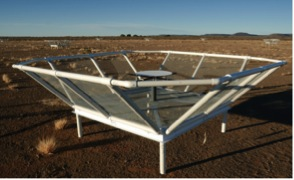
\includegraphics[width=\textwidth]{plots/paper_element.jpg}
%%		\Caption{-0.2in}{0.9}{-0.2in}{The PAPER element (provides a clean instrumental response as a function
%%		of frequency \citep{parsons_et_al2010,parsons_et_al2012b}, which is crucial to
%%		the foreground isolation shown in Figure \ref{fig:eor_pspec}.}
%%	\end{subfigure}
%%	\quad
%%	\begin{subfigure}[b]{0.46\textwidth}
%%		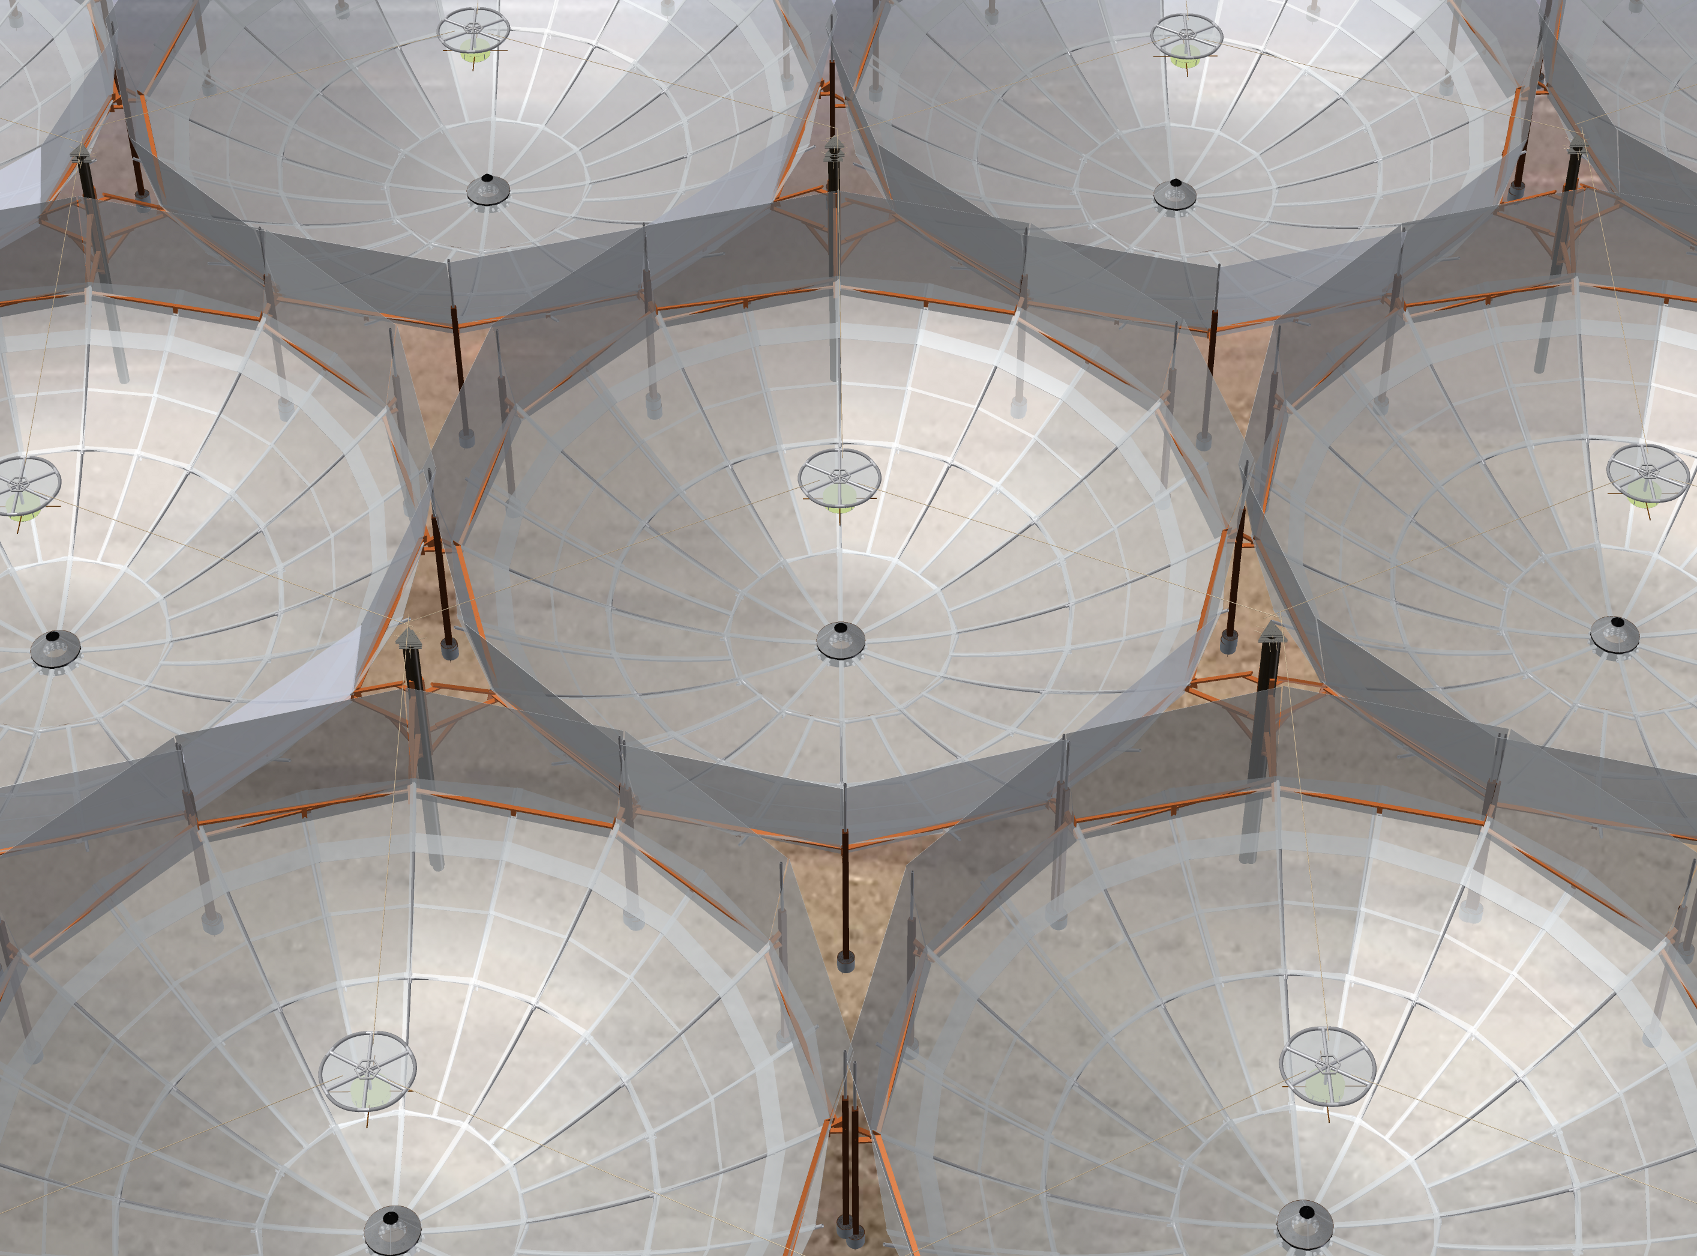
\includegraphics[height=1.75in]{plots/hera_dish.png}
%%		\Caption{-0.2in}{0.9}{-0.2in}{A 14m dish designed around the feed dramatically improves sensitivity while
%%		constraining the path length and amplitude of reflections to ensure that foreground 
%%		isolation is not substantially degraded.}
%%	\end{subfigure}
%%\Caption{-0.2in}{0.9}{-0.2in}{PAPER and HERA elements}
%%\label{fig:hera_dish}
%%\end{figure}
%
%The size of HERA-331 dishes optimizes cost for a fixed sensitivity and
%level of foreground isolation.  The associated reduction in the number
%of antenna elements to achieve a given collecting area, combined with
%the fact that these dishes have no moving parts, are built from
%inexpensive materials, and follow a simple construction that can be
%contracted locally, makes the cost of building HERA-331 substantially
%cheaper than was anticipated in the roadmap submitted to \nwnh\ for this
%stage of the program.   
%
%HERA leverages the technical heritage of PAPER, MWA and of CASPER\footnote{Collaboration for Astronomical
%Signal Processing and Electronics Research, a Berkeley-initiated worldwide open source community that is
%developing boards, firmware and software for the astronomical community} and incorporates a
%phased implementation to mitigate against risk.  The system, technology and phased approach is discussed below
%in more detail.

%\vspace{-0.25in}
\compress
\subsection{Instrument Design}
%\vspace{-6pt}
\label{InstDes}
%The HERA instrument design is very straightforward.  The element
%itself is a fixed zenith-pointing 14-meter segmented prime-focus paraboloid with a high screen
%to minimize cross-talk between elements (which are spaced 14.3 meters on a
%hexagonal grid).   The $f/D$ of
%the paraboloid is 0.32, so that the focal length, $f$, is less than 5 meters to meet the 
%standing wave specification at the delays of interest of more than 60 dB of attenuation at delays 
%greater than 50 ns.
%
%
%The active feed sends back the entire dual-polarization analog bandwidth on standard
%coaxial cable to an aggregation point called a ``node'', which services 
%about 15 antennas.  This cable length is kept short (35-m) to keep any standing
%wave contamination outside of the delay-space of interest for power spectrum
%measurements.  The node amplifies, filters, digitizes and transmits the signal data stream
%back to the central processing location (the Karoo Array Processing Building - KAPB).
%Figure \ref{fig:blockDiagram} shows a block diagram of the system.

\begin{figure}[t]
\centering
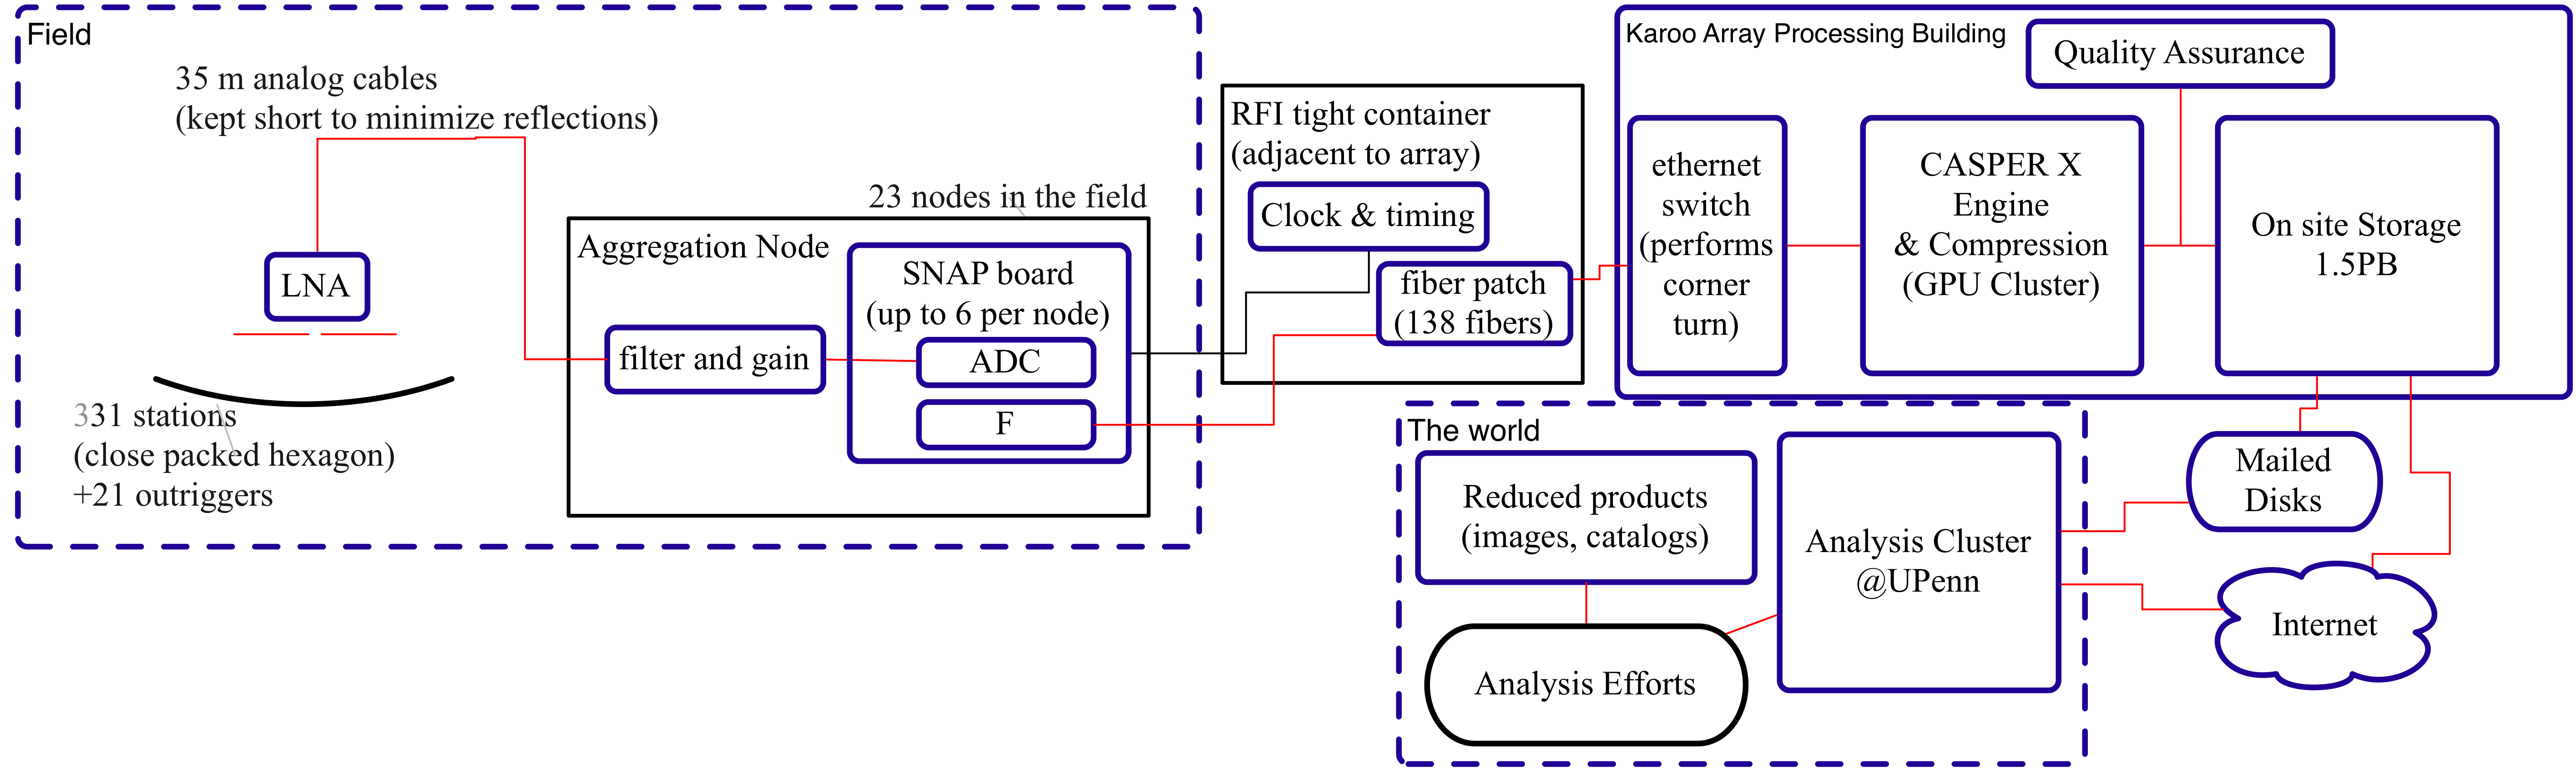
\includegraphics[width=\textwidth]{plots/Engineering/HERA_high_level_block_diagram.png}
\Caption{-0.75in}{0.9}{0in}{\small
Block diagram of the HERA system.}
\label{fig:blockDiagram} 
\end{figure}

As shown in Figure \ref{fig:blockDiagram}, the HERA instrument has a straightforward signal
path from antenna elements
with active feeds, to nodes that digitize and aggregate signals onto an optical network,
and on to a processing building where signals are correlated, and data are stored, compressed,
and shipped to a computing cluster located at U. Pennsylvania (UPenn). 

\compress
\subsubsection{Antenna Element}
%\vspace{-6pt}

The novel design of HERA's antenna element
(Fig. \ref{fig:hera_dish}, right panel) represents a critical advance
that enables HERA to achieve its science goals.  This 14-m
fixed zenith-pointing parabolic dish yields more than 10 times the
sensitivity of an MWA tile (and more 20 times
that of a PAPER element), but does so without substantially degrading
our ability to isolate and remove foreground emission on the basis of
spectral smoothness.  As described above, this is done by limiting by 
the timescale of signal delays and reflections to under 120 ns.

Since the time it takes radio emission to propagate between adjacent antennas 
represents a significant portion of this time budget, HERA elements must be placed close together.
Recent work characterizing foregrounds suggests that 
antenna separations of $8\lambda \approx 15$m are
well-behaved to current limits \Mycitep{pober_et_al2013,parsons_et_al2013}. This influences our
choice of a 14-m dish diameter,
which incurs 42 ns of signal delay between adjacent antennas.
The focal height (4.5 m) derives from the illumination pattern of the prime-focus
feed, and the fact that reflections
between the feed and the element%,
%caused by imperfect impedance matching between the feed electronics and free space, 
can introduce additional signal delay. 
%With a splash cone underneath the feed to scatter reflections, we assume -20 dB
%attenuation per reflection, so that after three traversals (13.5 m; 41 ns), reflections from
%foreground emission are below the expected level of the 21~cm reionization signal.
Additional measures, such as a splash cone underneath the feed, screens that isolate feeds from one another, and using
non-metallic cabling and poles for supporting the feeds, are all aimed at minimizing
the potential for additional sources of signal reflections.
The total signal delay associated with the HERA dish design is estimated at 83 ns, leaving
headroom for reflections arising in the analog signal path.

Cost is another design constraint, including the price of construction
materials, assembly in a remote area, and maintenance over the operational
lifetime of the array.  Care has been taken to select robust and inexpensive
construction materials (PVC, concrete, utility poles, 0.25" wire cloth) and an assembly methodology that delivers the required positional
accuracy of 10 cm and surface accuracy of 2 cm given standard expertise in construction
practices for the subcontracted teams that set the poles and construct the
elements in the field.  
%JCP: "required positional accuracy" -- what drives the requirement?
Given the sensitivity and signal delay requirements, the size of HERA
dishes optimizes a global costing curve that includes the costs of the elements,
the signal path, correlation, data storage, and processing.

% ARP: removing this figure, since it appears in project management plan
%\begin{figure}[h]
%	\centering
%		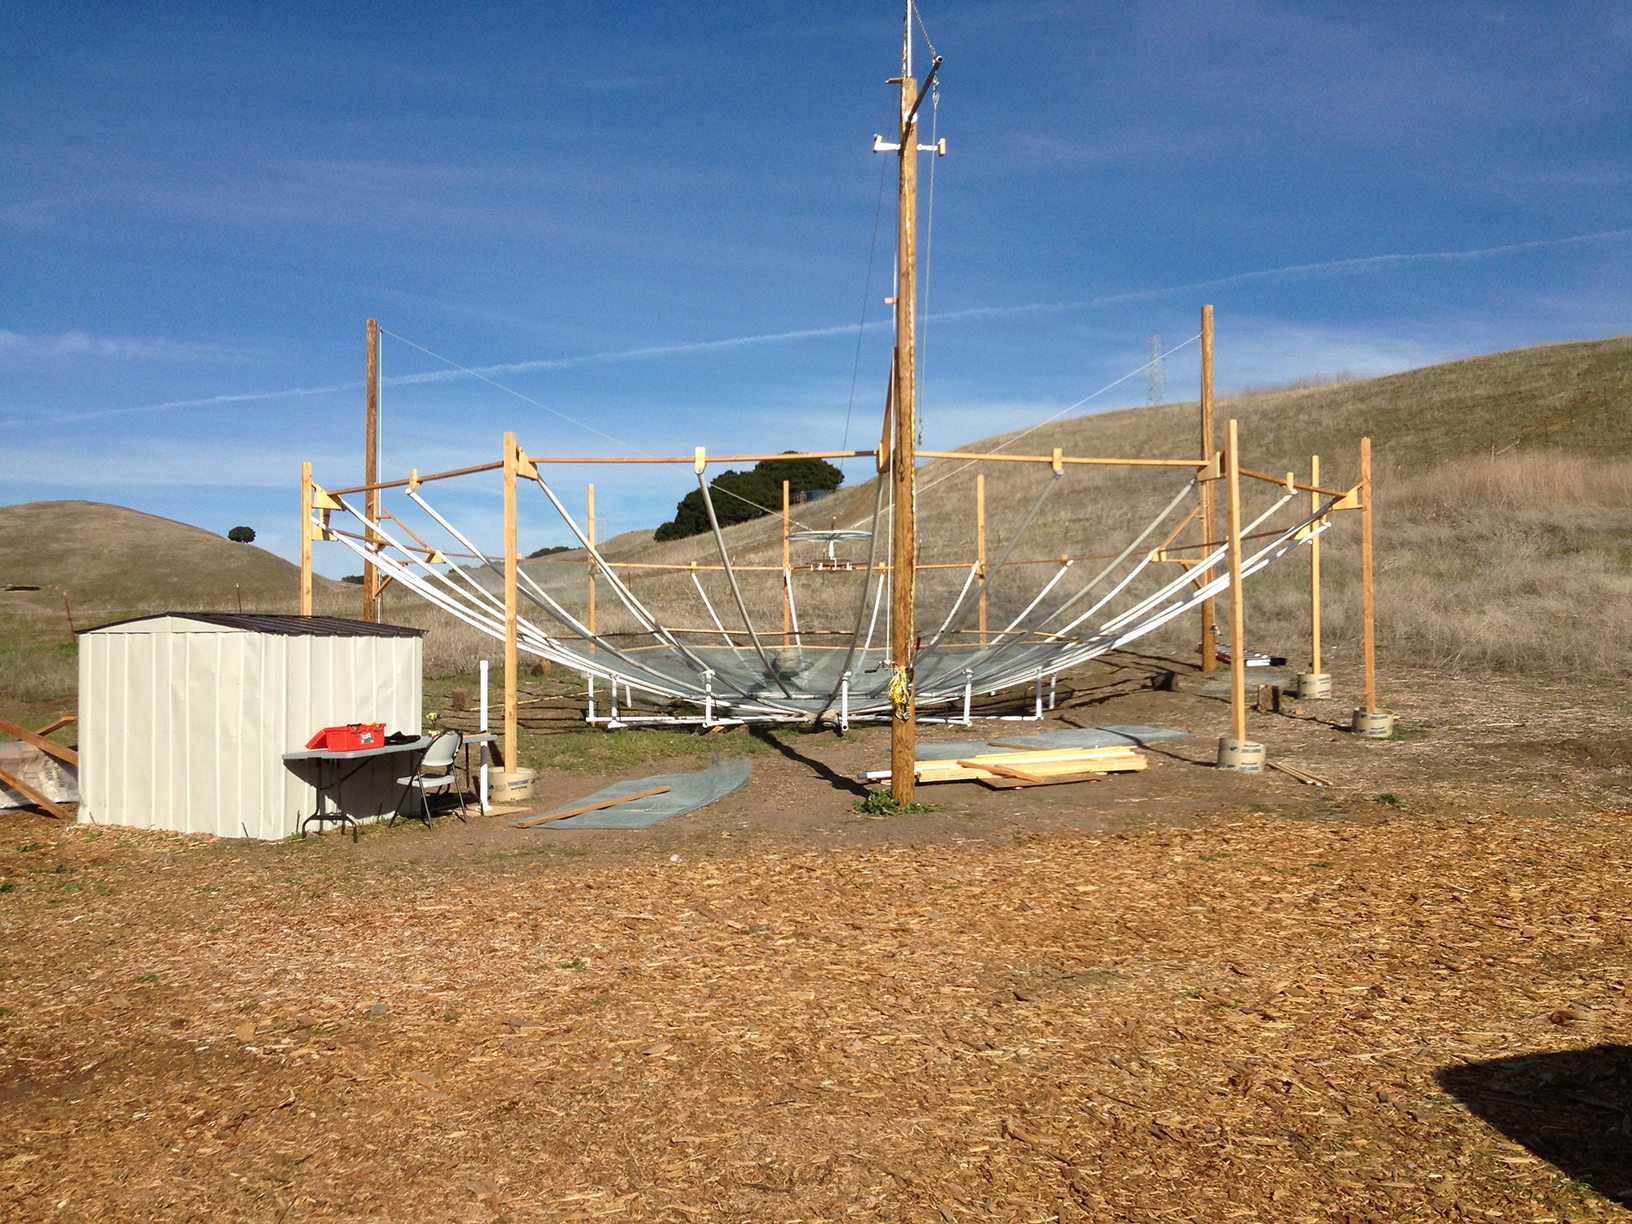
\includegraphics[width=0.46\textwidth]{plots/heracles.png}
%		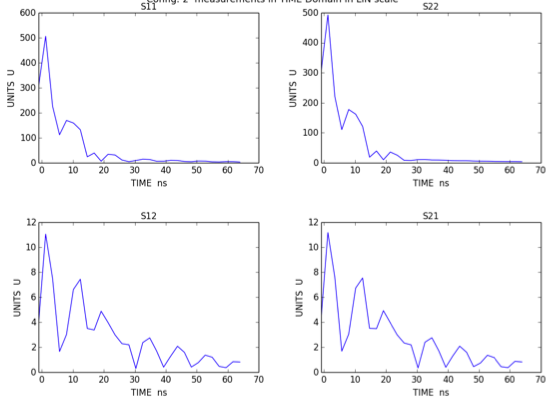
\includegraphics[width=0.46\textwidth]{plots/Engineering/heraclesNA.png}
%	\caption{\small
%		The construction prototype element in California (left) with preliminary 
%        reflection measurements (right).
%} \label{fig:heracles}
%\end{figure}

%As illustrated in Figure \ref{fig:heracles}, 
A first prototype of the HERA dish is nearly completely constructed.  In this
proposal, UC Berkeley and NRAO 
lead the incorporation of lessons from the
construction process and reflectometry tests into the design.
Two further prototype elements are constructed in the first year alongside the existing
PAPER array in Green Bank, WV,
for on-sky measurements of the beam pattern and spectral 
response.
These measurements are coupled with full electromagnetic modeling to test
and refine the element design prior to a Critical Design Review at the end of the first project
year.  Three revised elements are then constructed in South Africa, involving
lead members of the construction subcontract teams for a Project Readiness Review.  %Thereafter,
%element construction will proceed continously through the second and third project years during the day,
%with a staged incorporation of new elements for night-time observing.

%The elements are
%also nearly abutting one another, which allows for sharing of physical support
%infrastructure.


% ARP: lack room for this figure.
%\begin{figure}[h]
%	\centering
%	\begin{subfigure}[b]{0.46\textwidth}
%		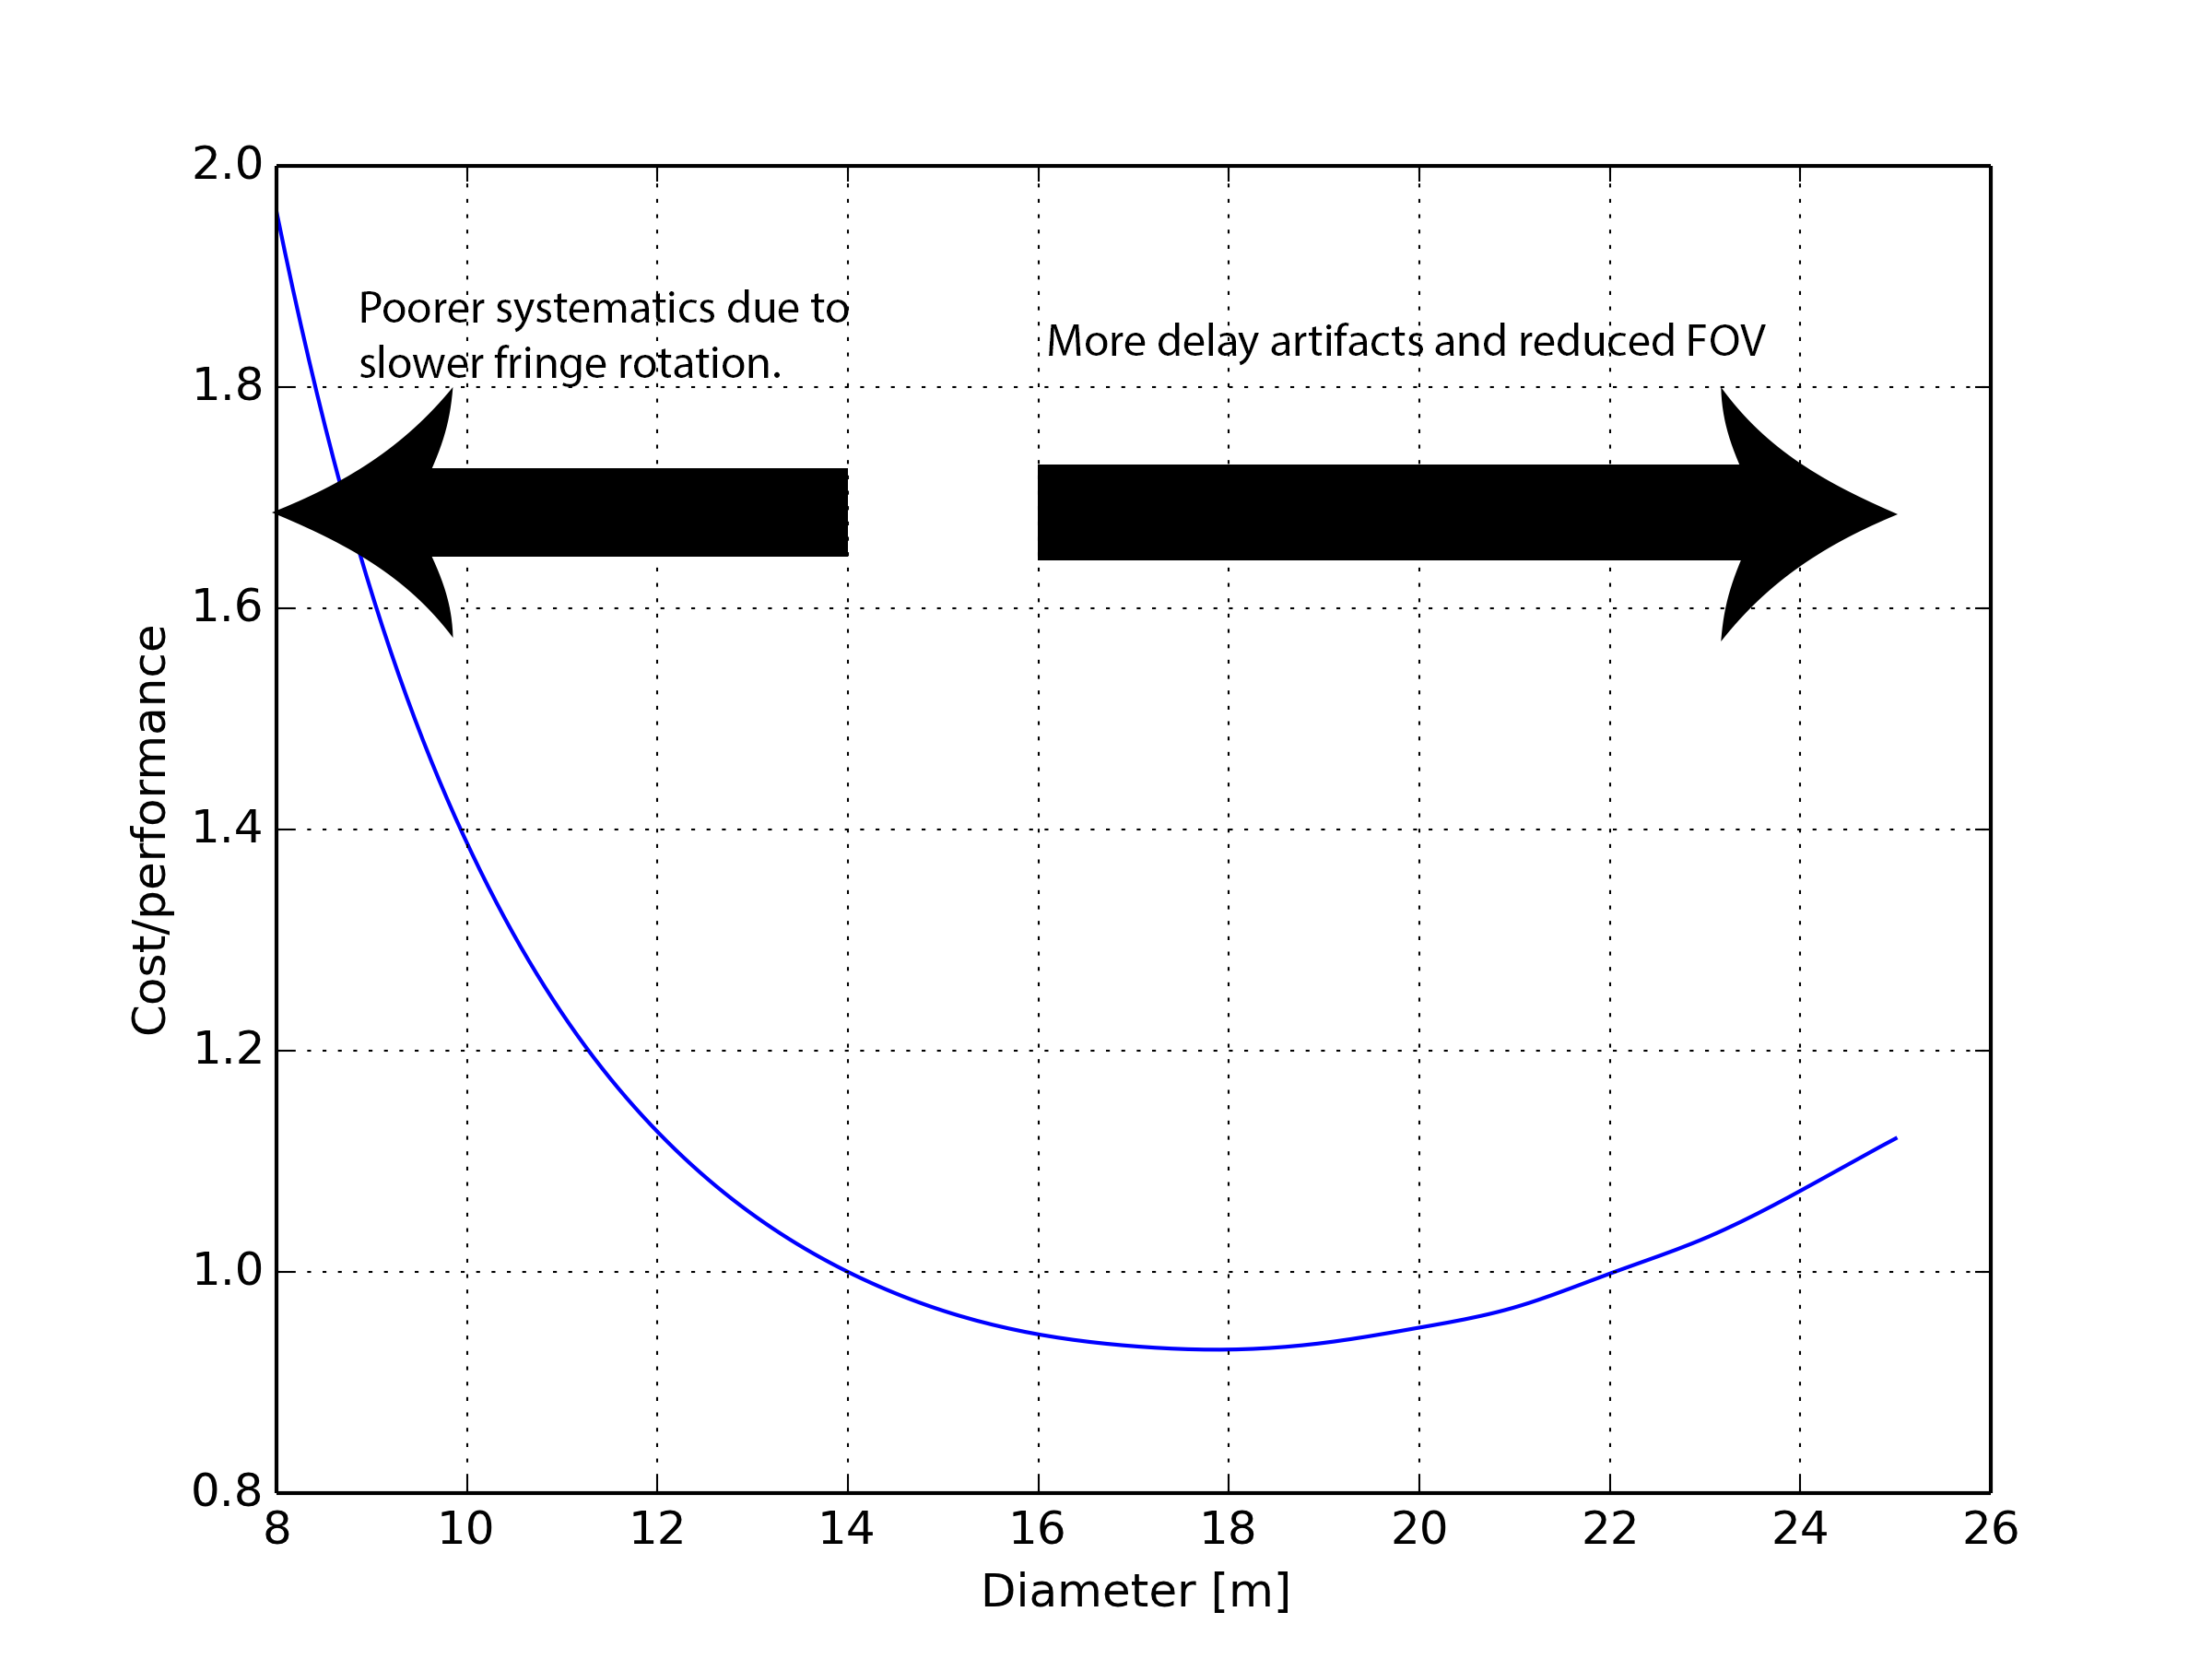
\includegraphics[width=0.9\textwidth]{plots/Engineering/nvsd.png}
%		\caption{Costing model for a fixed sensitivity and varying the diameter.   The arrows indicate the regions of 
%				increasing systematics and delay-space contamination.}
%		\label{fig:nvsd} 
%	\end{subfigure}
%	\quad
%	\begin{subfigure}[b]{0.46\textwidth}
%		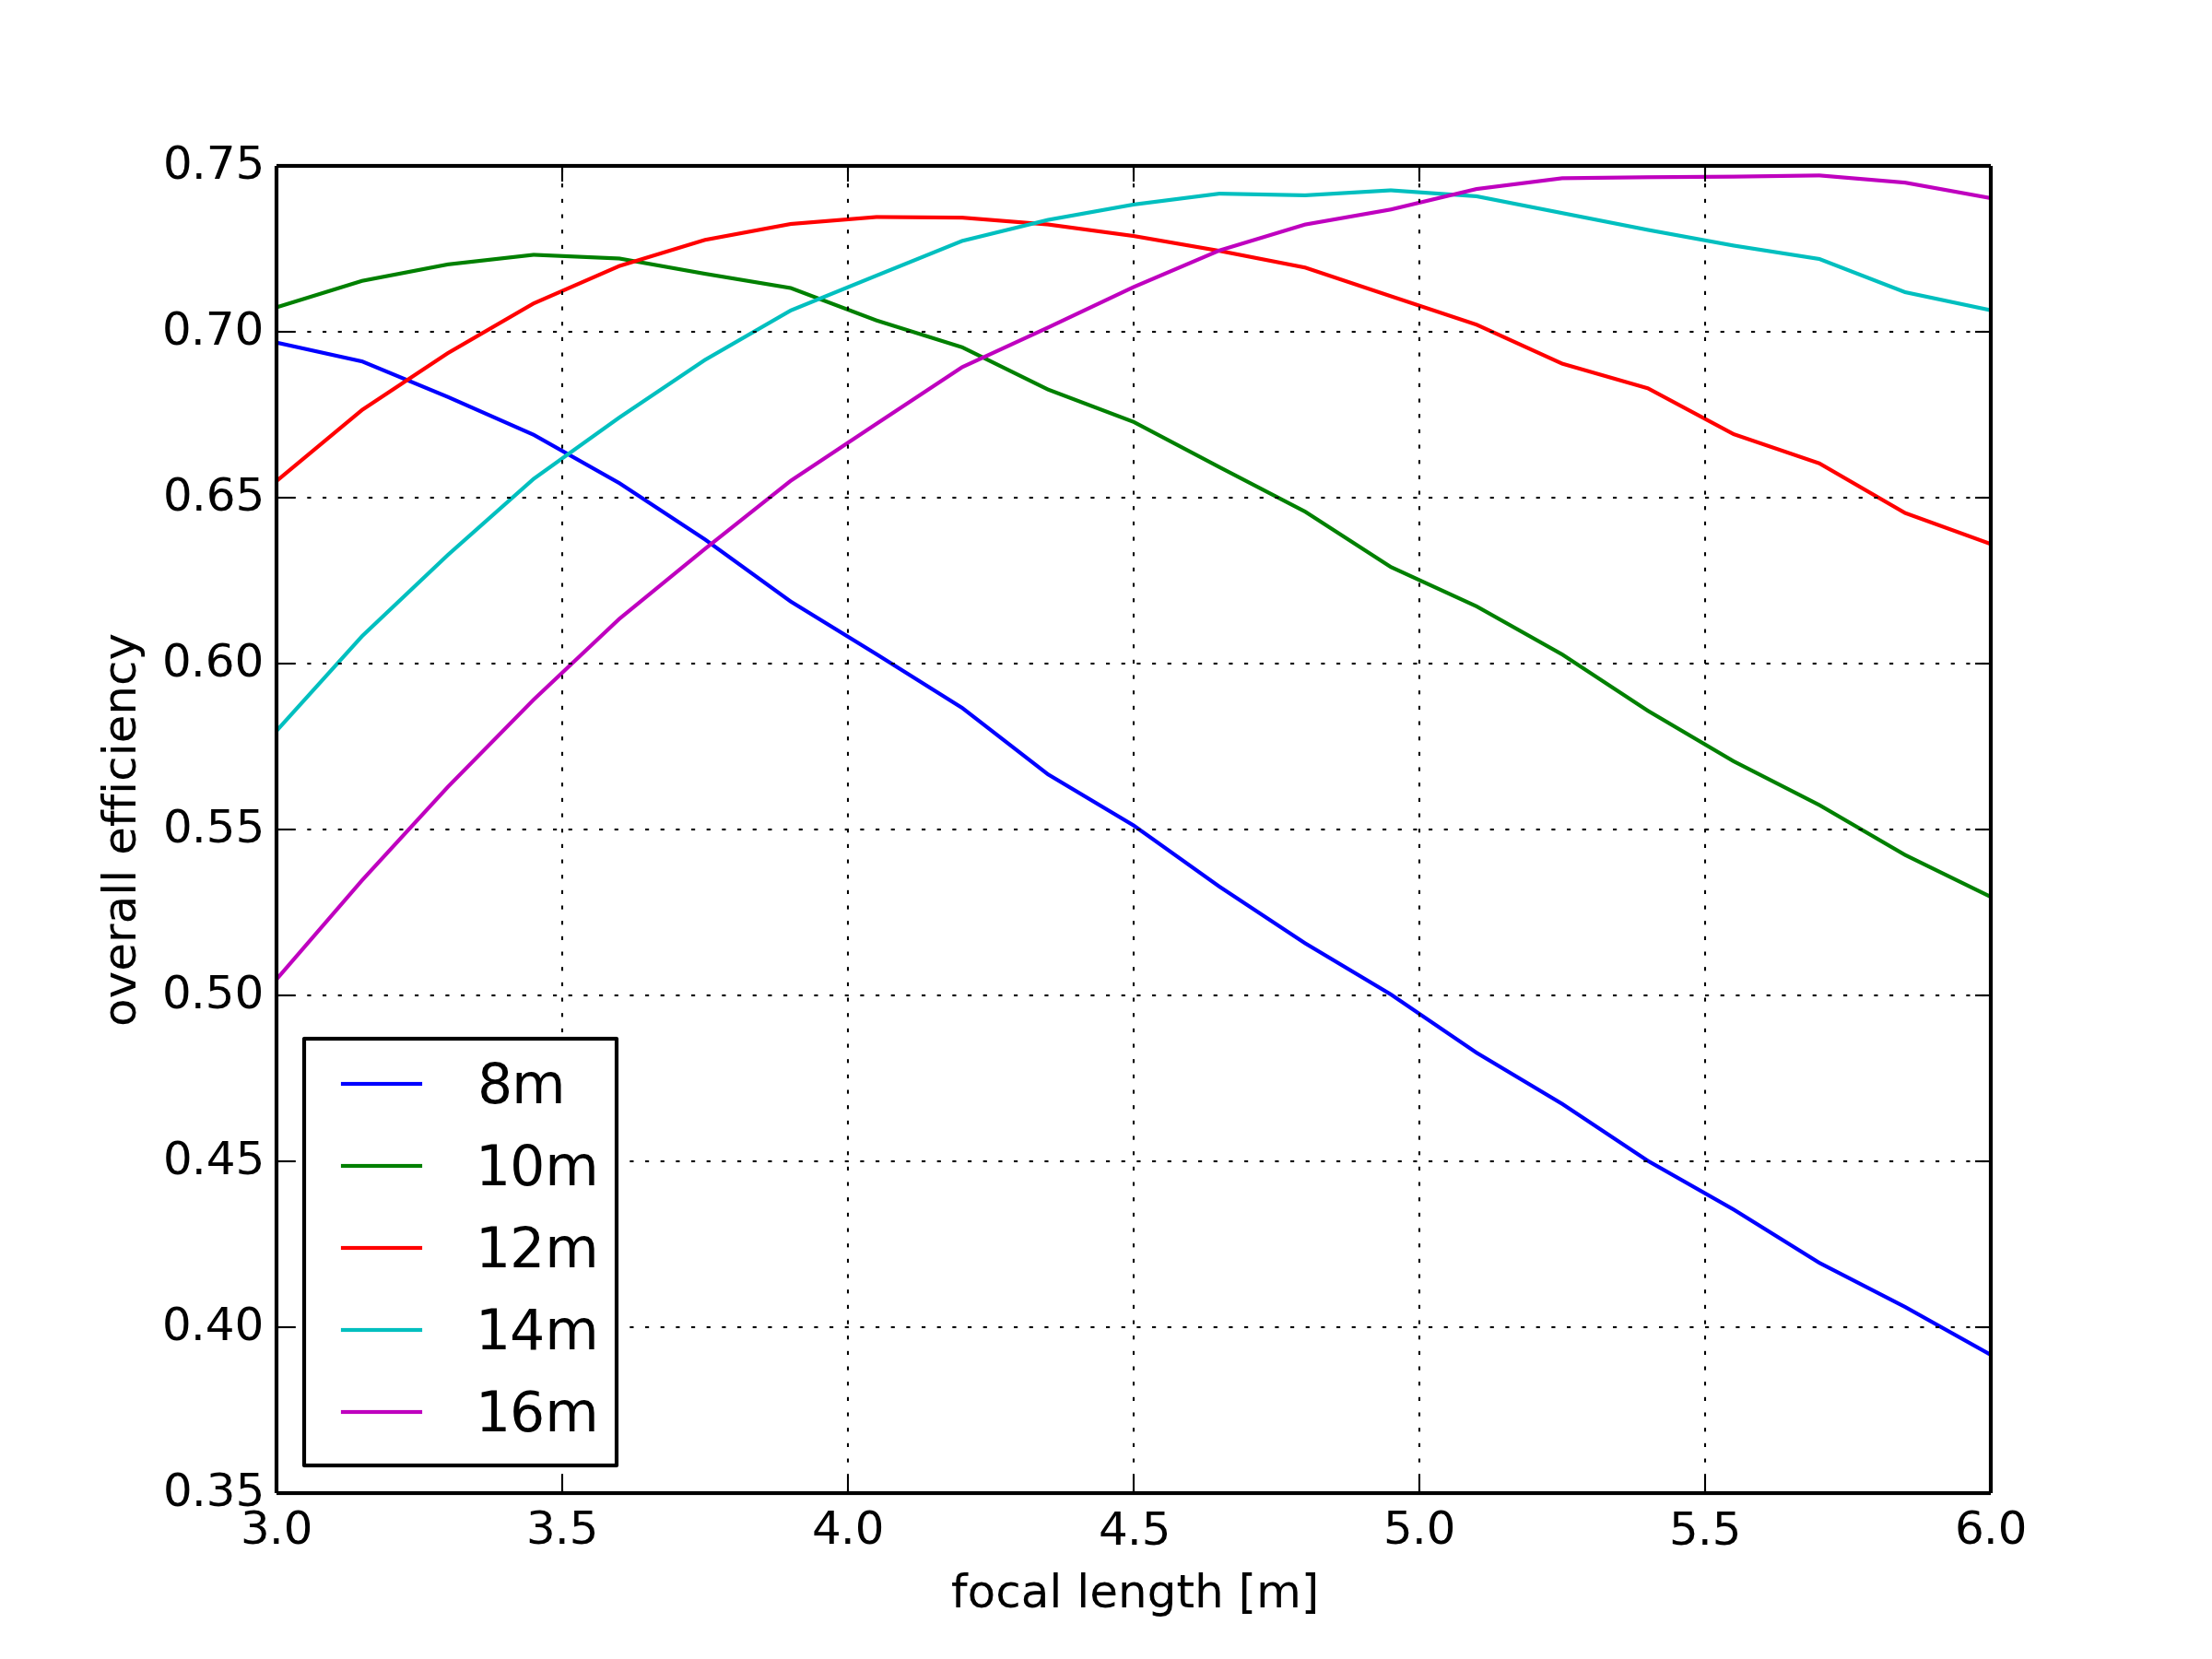
\includegraphics[width=0.8\textwidth]{plots/Engineering/focalEff.png}
%		\caption{Analytical model efficiency of a parabolic element as a function of focal height and diameter.   The delay 
%				contamination specification is $f<5$m.}
%		\label{fig:disheffic}
%	\end{subfigure}
%	\caption{Cost and performance variational analysis data for the element.}
%\end{figure}

% FOLLOWING SEEMS TOO DETAILED FOR A PROPOSAL
%To distinguish between measured sky delays and instrumental-induced delays at a required threshold ($R_T$) dB, 
%we need sufficient attenuation of the reflected signals at a given focal length ($f$) at a specified delay ($\tau_{d}$).  Assuming a conservative simple model that the magnitude of the reflection is attenuated by $A$ dB at each reflection 
%we see that for a delay length limit of $\delta_{d}=c\tau_{d}$ and focal length $f$,  the required focal length is
%
%\begin{equation}
%f < \left(\frac{A}{R_T}\right)\delta_d.
%\end{equation}
%
%Using nominal values of $R_T$ =  60dB (an order of
%magnitude below where EoR is predicted to be below foregrounds) at delays
%corresponding to the time it takes travel 15m and a net attenuation of 20 dB per reflection, 
%we find that the focal length should be less than about 5 m.  Free-space loss effects would 
%increase that value, loosening the constraint.
%DETAILEND

%In addition to the constraints given by the element itself, the HERA element size is
%also influenced by the location of the ``knee'' in the EoR power spectrum \citep{lidz_et_al2008}
%The EoR power spectrum has an upward slope for low $k$-modes which levels off
%around $k=0.15 h$/Mpc %(see fig blah). 
%Working inside this $k$-mode would be beneficial due to the fact foregrounds are
%less problematic. This poses a problem because without knowing the
%width of our foregrounds, we can't say for sure which $k$-modes (in the power
%spectrum) are corrupted. This uncertainty, coupled with increasing systematic affects for shorter 
%baselines (hence smaller diameters), favors larger diameter antennas.

%% ARP: no room for this figure.
%\begin{figure}[h]
%	\centering
%	\begin{subfigure}[b]{0.46\textwidth}
%		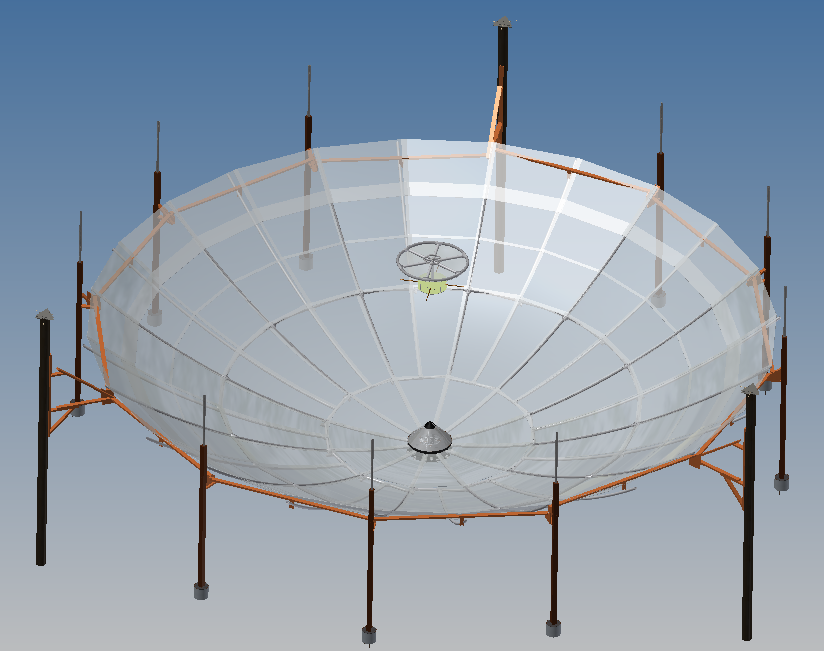
\includegraphics[width=0.85\textwidth]{plots/dish.png}
%		\caption{CAD model of 14m dish with screening and some supports removed to show detail.}
%		\label{fig:dish} 
%	\end{subfigure}
%\quad
%	\begin{subfigure}[b]{0.46\textwidth}
%		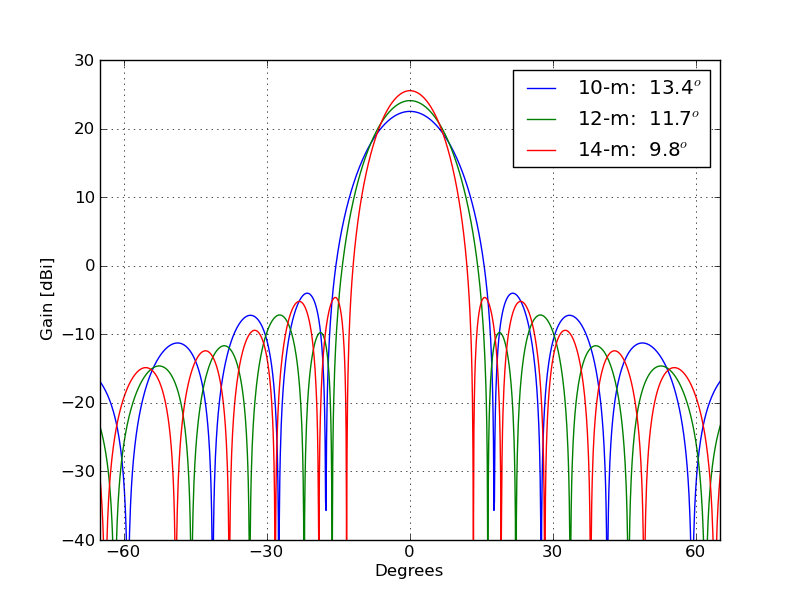
\includegraphics[width=\textwidth]{plots/Engineering/hera_beam.png}
%		\caption{Analytical model beam patterns at 10m, 12m and 14m.}
%		\label{fig:beam} 
%	\end{subfigure}
%	\caption{HERA element and beam pattern.}
%\end{figure}

%The $k$-mode for a $14m$ baseline is $k = 0.023$, given by $k_{H} =
%\frac{B}{c}\frac{dk}{d\eta}$, where $B$ is the length of the baseline, 14m in
%our case, $c$ is the speed of light, and $\frac{dk}{d\eta}$ is the cosmological
%transfer function from delays to $k$-modes. In addition, narcissistic
%reflections add into our $k$ budget as well. The $f$ and $D$ choices above provide a $k$ budget for
%foreground widths to be within $\Delta{k}\sim{0.1}$. Testing these hypothesis
%and again, finding a compromise between maximum sensitivity, foreground budget
%will be key to testing and constructing the required element. Foreground width constraints
%are still an area of active research \citep{pober_et_al2013}.

% The core defining elements in this design are the central hub and three tall support poles.  Three intermediate 
% support posts are installed between each pair of poles.  A 2$^{\prime\prime}$ PVC spar of 24.1$^{\prime}$ 
% terminates at each pole and post.  These spars are supported at each end and one point in the middle at the 
% proper height and angle.  The intervening PVC pipe essentially acts as a smoothing filter between those 
% points, noting also that a beam with point loads attains nearly the quadratic shape desired.  The CAD model is 
% shown in the right panel of Figure \ref{fig:hera_dish}.  
% 
% The tall ($\sim$ 7m) poles provide locational accuracy (in all three dimensions) for the overall array installation.  
% Using conventional commercial pole-installation techniques the poles are installed first for the entire array.  
% Note that every pole except for the edge poles are shared by three antennas.  A standard theodolite can 
% then be used to mark a known level height on all three poles.  These locations are then used with tensioned 
% lines to define the center of that element and the hub is positioned at that location using a jig.
% 
% The hub uses concentric commercially available ``sonotube'' forms (circular cardboard forms for concrete pillars) 
% and PVC sleeves to hold the PVC spars and PVC supports.  The retaining holes may be accurately cut into 
% the forms, sleeves installed and concrete poured to make a simple hub to the desired accuracy.  The jig holds 
% the concentric rings in place and allows it to be centered by tensioned lines while the concrete is poured.  
% When the concrete cures one can then transfer an accurate offset from the dish vertex back to the poles.
% The intermediate posts are then located by the support sub-assemblies attached to the poles and posts along 
% with the rim sub-assemblies.  These are positioned and a small pier is poured to locate them.  After spar support 
% pieces are installed on the posts, the spars themselves and the metal cloth can be installed.
% 
% The feed is held off the three tall poles using tensioned lines to accurately locate it over the hub.  A precise 
% length of kevlar rope holds the feed down to the hub at a precise focal point.  The RF cables follow the line 
% down and out to the analog-to-digital converters and correlator.  
% 
% To minimize cross-talk, metal screens are strung between every pole/post, which go to the level of the feed.  
% The dishes have a rim-to-rim spacing of 30cm to allow the screen to be slightly angled to minimize standing waves.

\compress
\subsubsection{Array Configuration}

\begin{figure}[t]
\centering
		%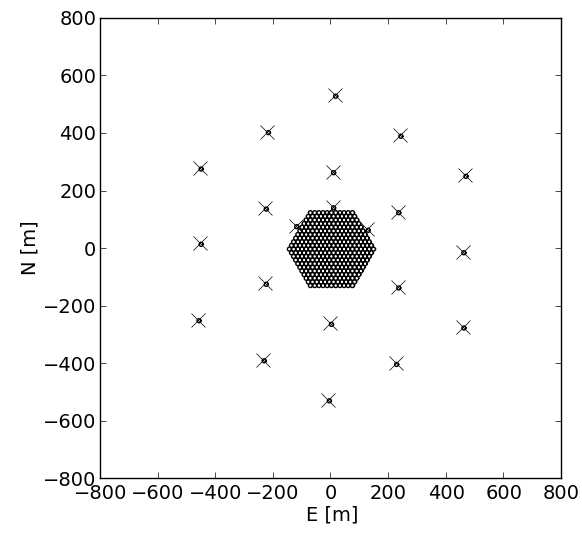
\includegraphics[height=2.5in]{plots/HERA_331_pos.png}
		%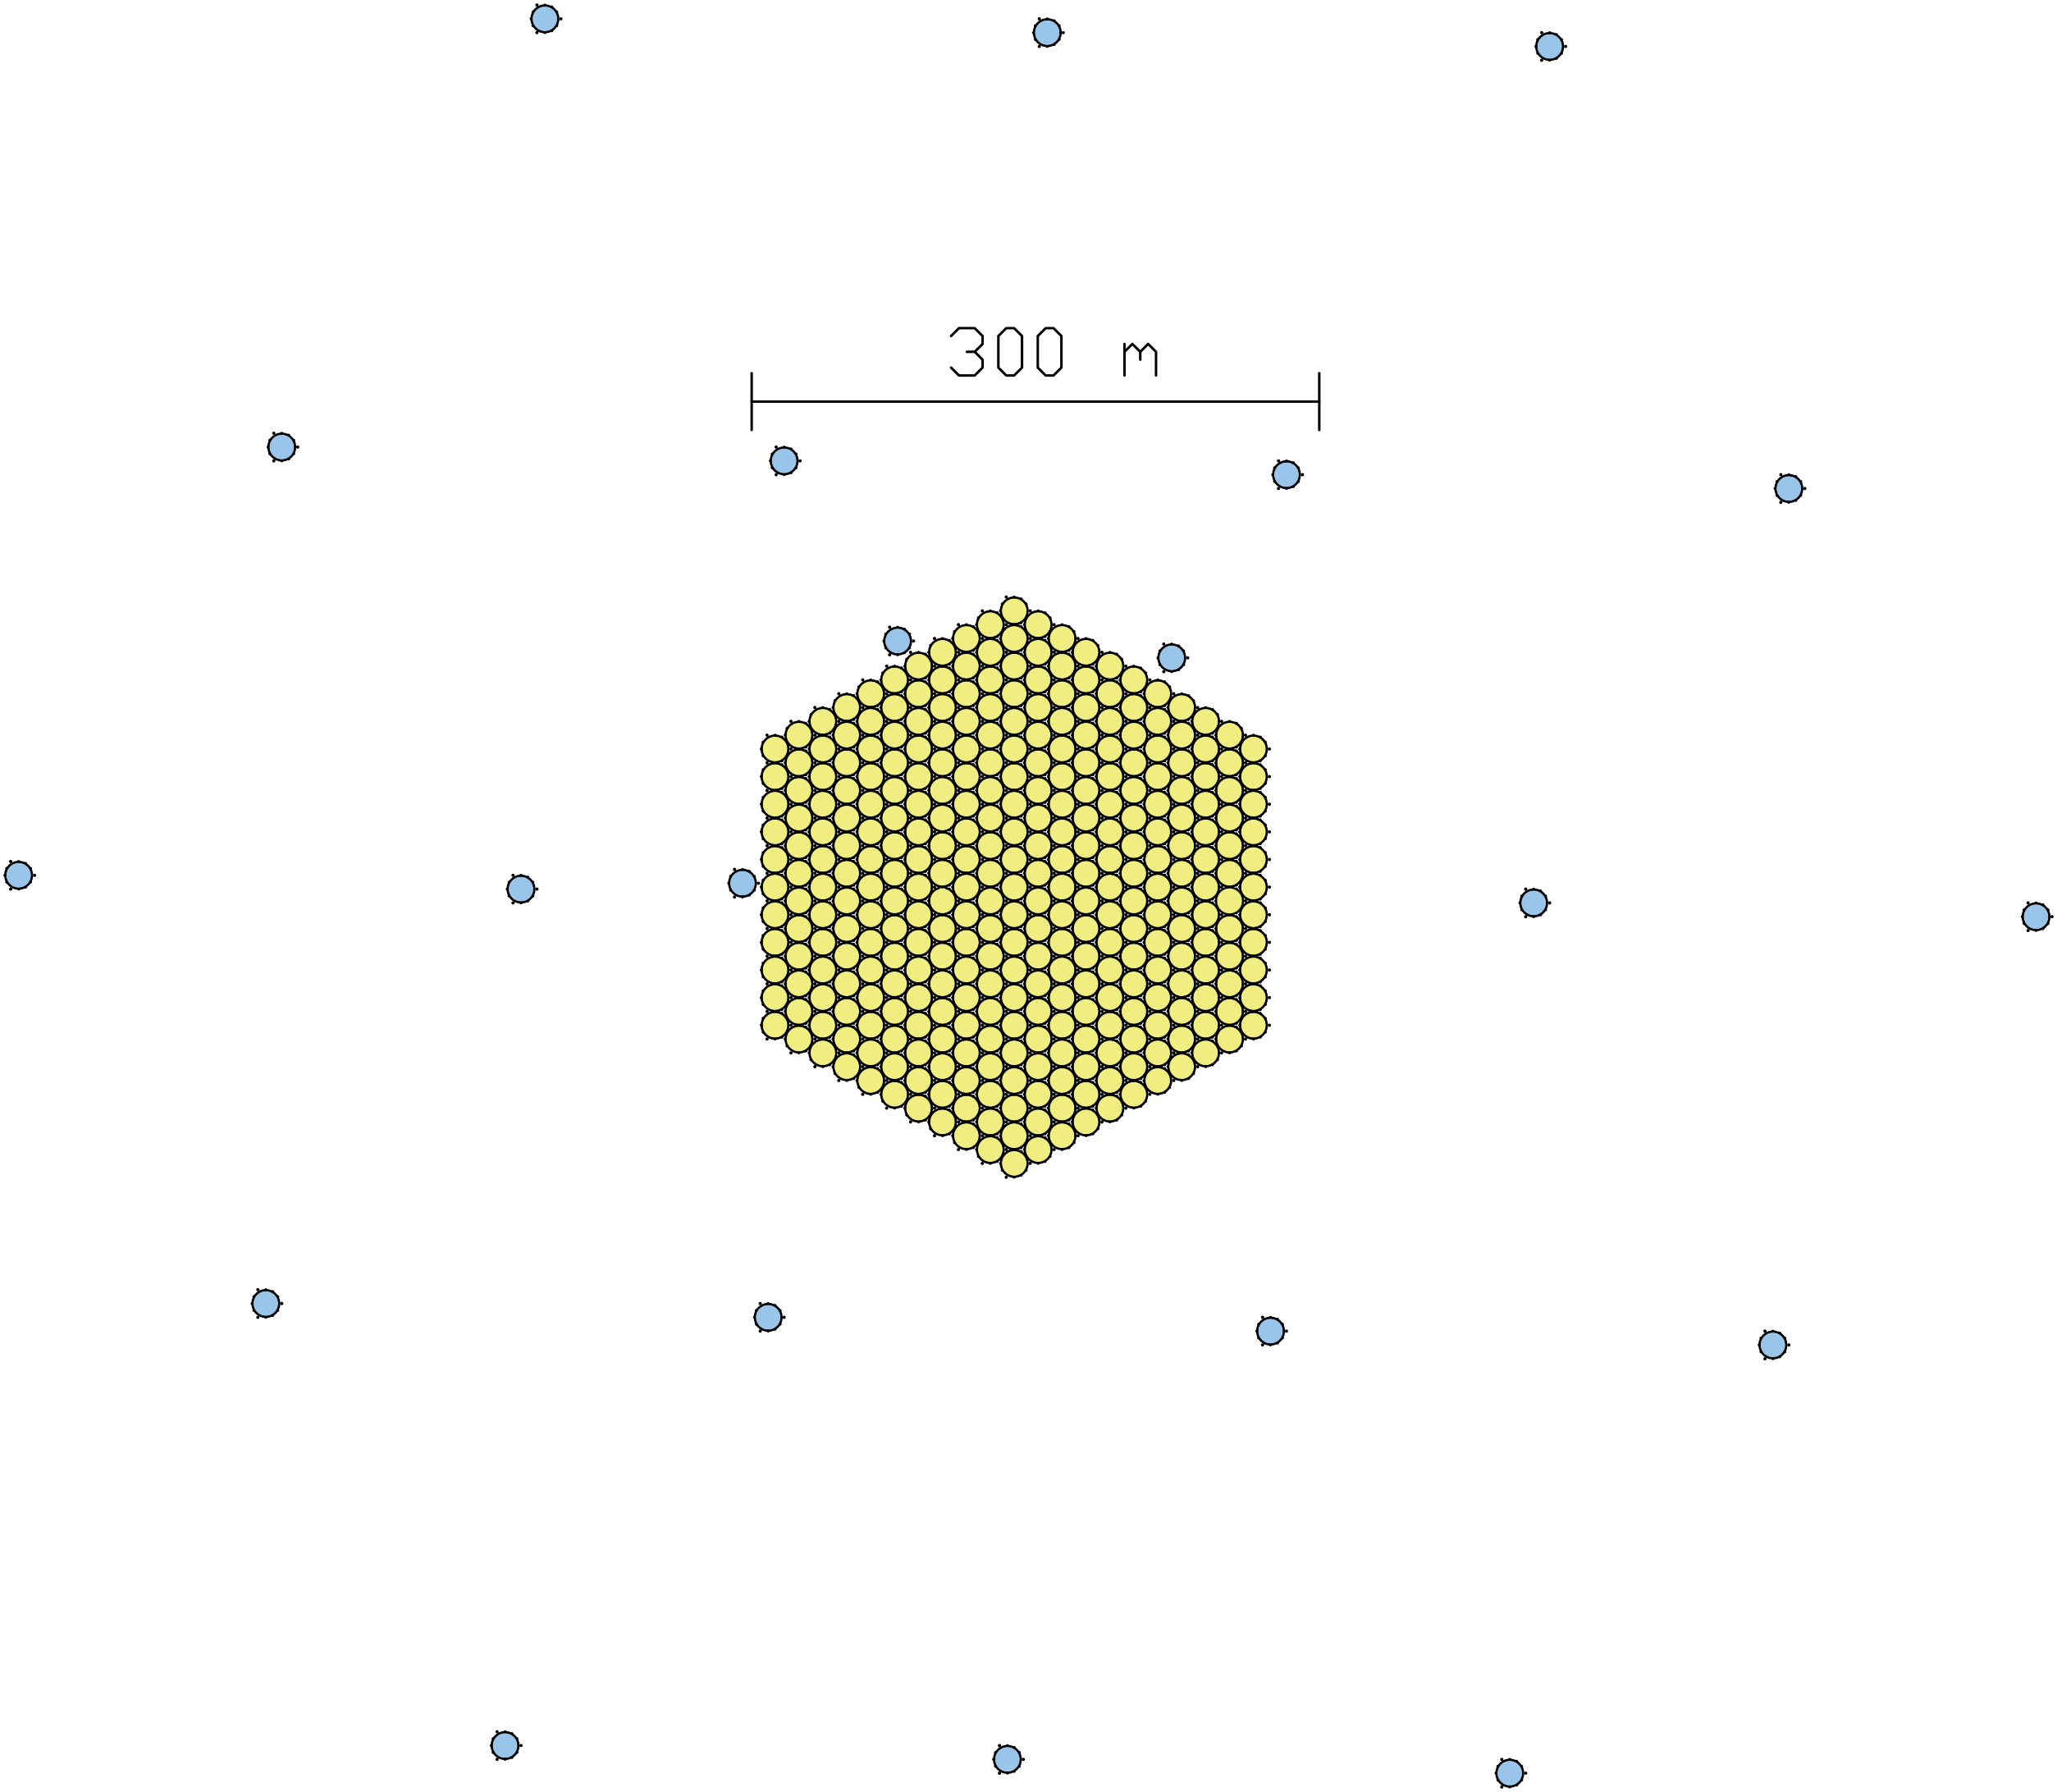
\includegraphics[height=2.1in]{plots/hera352rot.png}
		%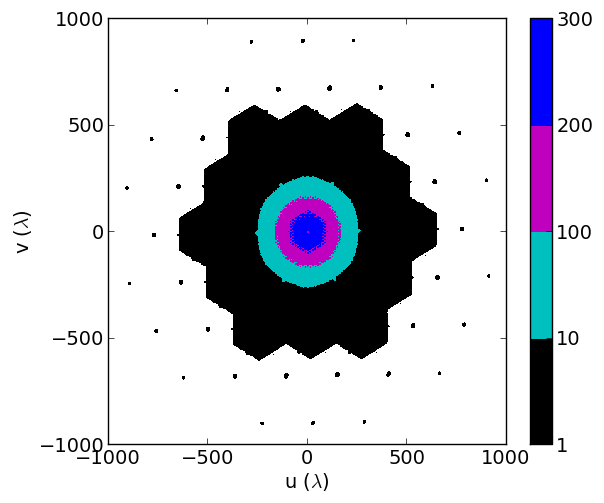
\includegraphics[height=2.1in]{plots/HERA_331_uv_clipped.png}
		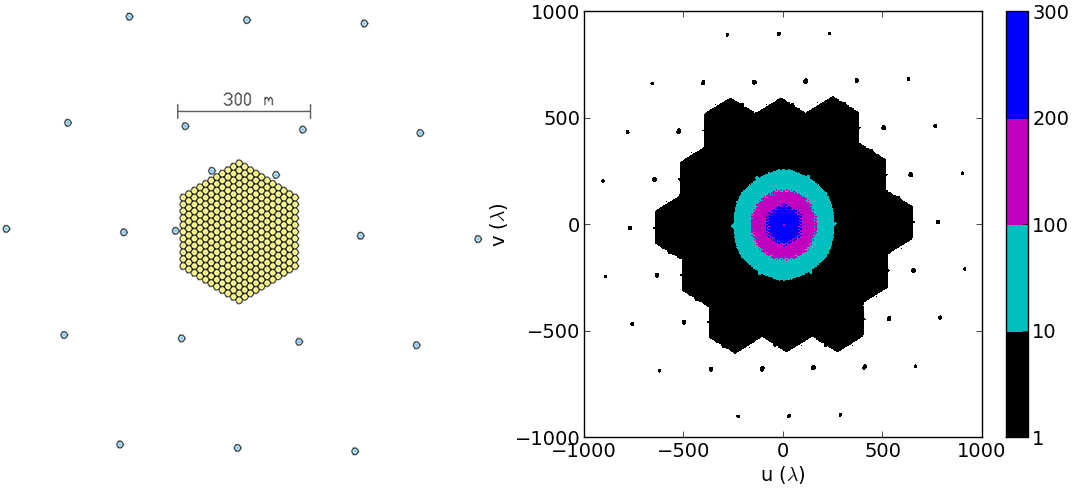
\includegraphics[height=2in]{plots/config_uv_consolidated.png}
\Caption{-0.15in}{0.9}{-0.1in}{\small
Left: Configuration of HERA-331, with 331 dishes in a maximally-dense hexagonal core (yellow) and 21 outrigger dishes (blue).  Right: The resulting $uv$-coverage is fully-sampled to $\sim 400\lambda$ 
}\label{fig:uv_coverage}
\end{figure}

For HERA-127 and HERA-331, elements are arranged in a compact hexagonal grid.
This configuration minimizes antenna separation, which is critical for meeting
the science requirements for foreground isolation, and 
produces a highly redundant sampling of the $uv$ plane.  As described in
\S\ref{sec:Lessons}, redundant configurations have been employed by PAPER to
boost sensitivity \Mycitep{parsons_et_al2012a}, with the added benefit that they
greatly facilitate fast and accurate calibration
\Mycitep{liu_et_al2010,parsons_et_al2013}.  Placing HERA elements in a
grid allows certain construction components to be re-used between antennas,
reducing cost, and improving the accuracy of element placement.  HERA-331 
is a build-out of HERA-127 from the eastern edge.

The HERA-331 core has excellent
imaging capability that can be leveraged for developing foreground suppression techniques
to improve access to the 21~cm reionization signal 
(Fig. \ref{fig:eor_pspec}, black).
This capability is augmented with 21 outrigger elements.  These outriggers
combine with the dense core to generate a fully
sampled $uv$ plane out to 400$\lambda$.  While outriggers on the southern half of the array are
placed in alignment with the hexagonal grid in the core, elements on the northern side are
shifted off-grid to sample the $uv$ plane at sub-aperture scales.
This sampling strategy helps eliminate grating lobes in the
synthesized beam and provides information for
calibrating and correcting direction-dependent antenna responses.  This capability may
be used to match polarization beams and minimize
polarization leakage.
% XXX once we mention polarization leakage, we better hit it head on...


\compress
\subsubsection{Analog Signal Path}
\vspace{-6pt}

\begin{figure}[t]
    \centering
        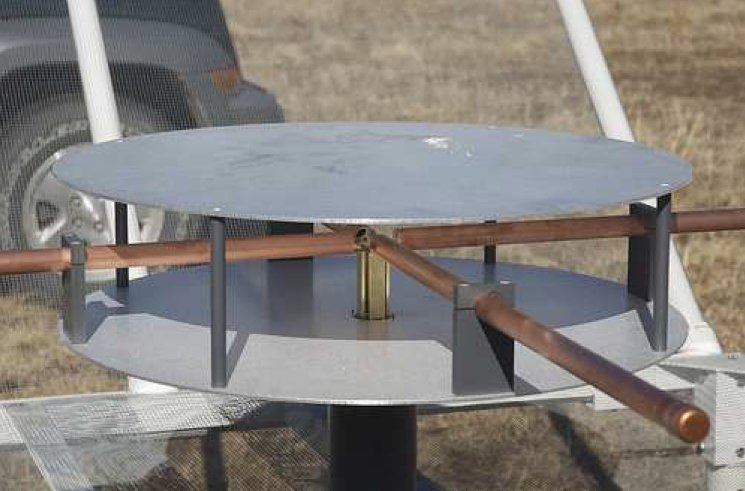
\includegraphics[height=1.5in]{plots/new_antenna_closeup.jpg}
        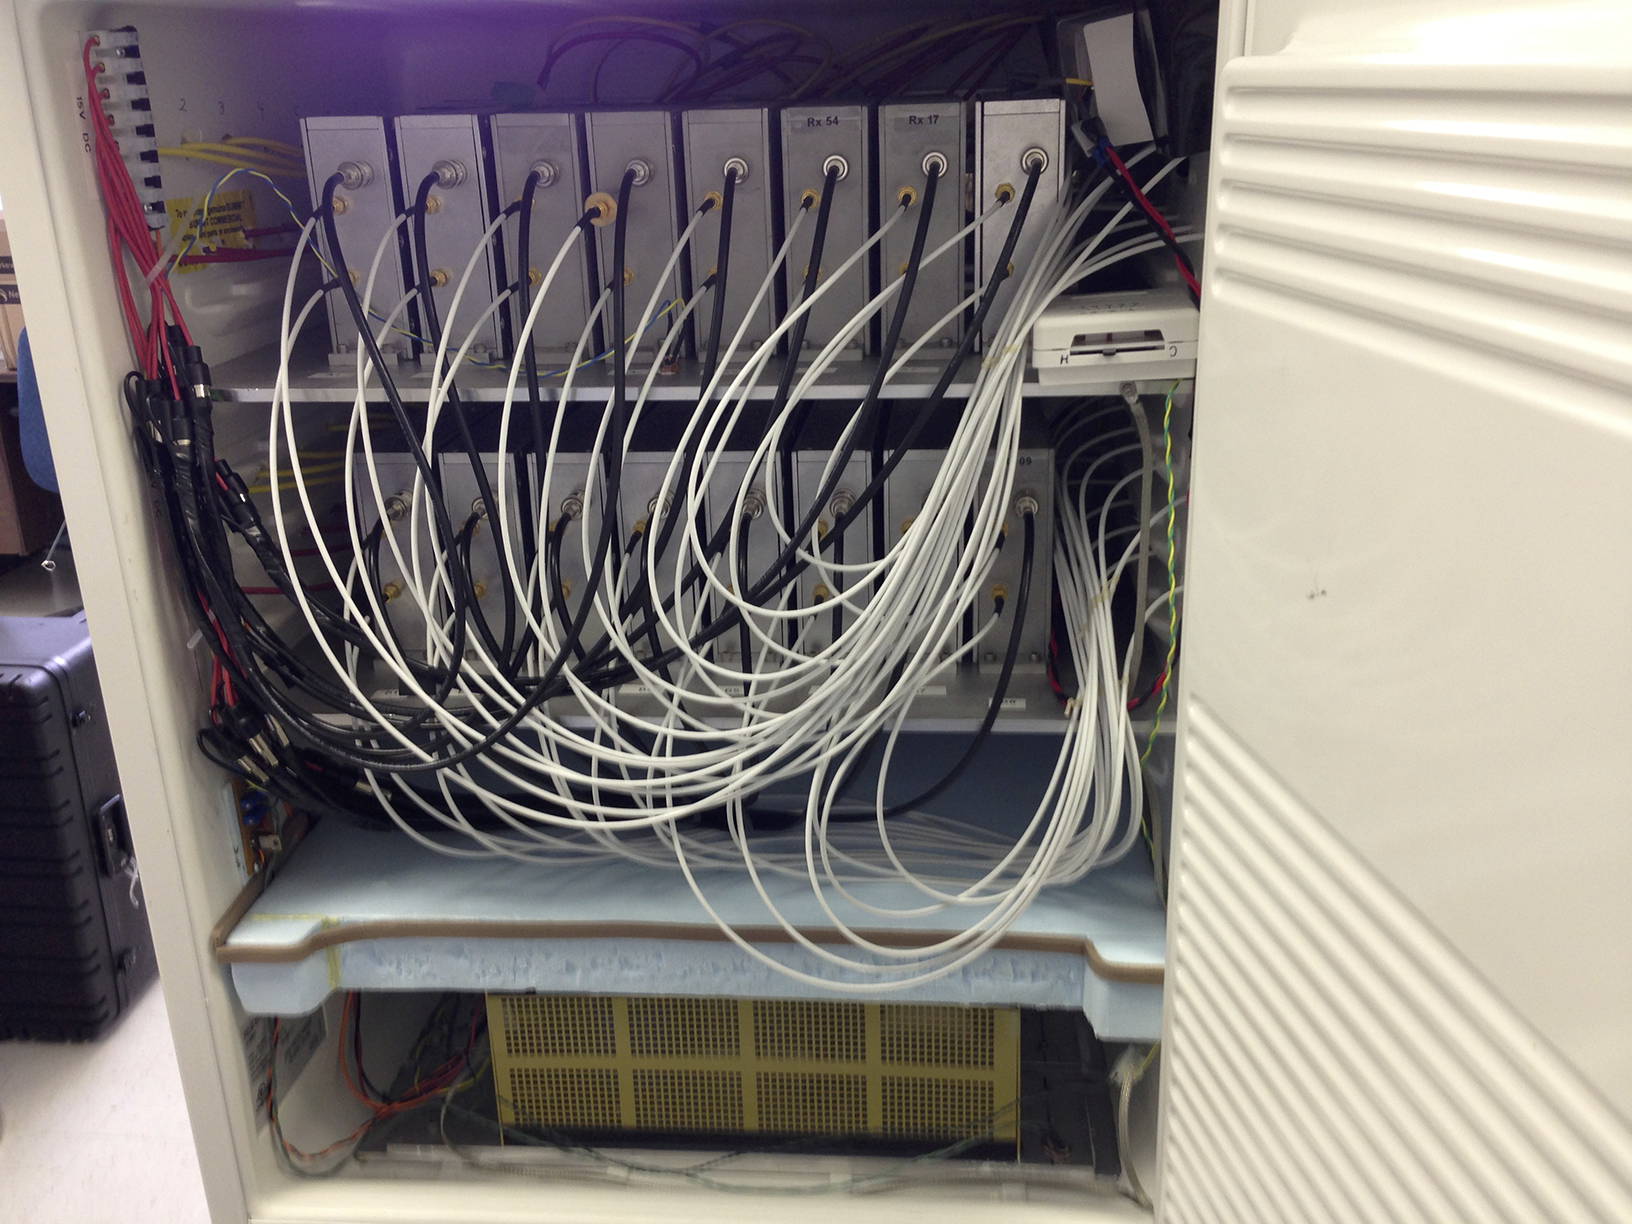
\includegraphics[height=1.5in]{plots/Engineering/recv_node.png}
        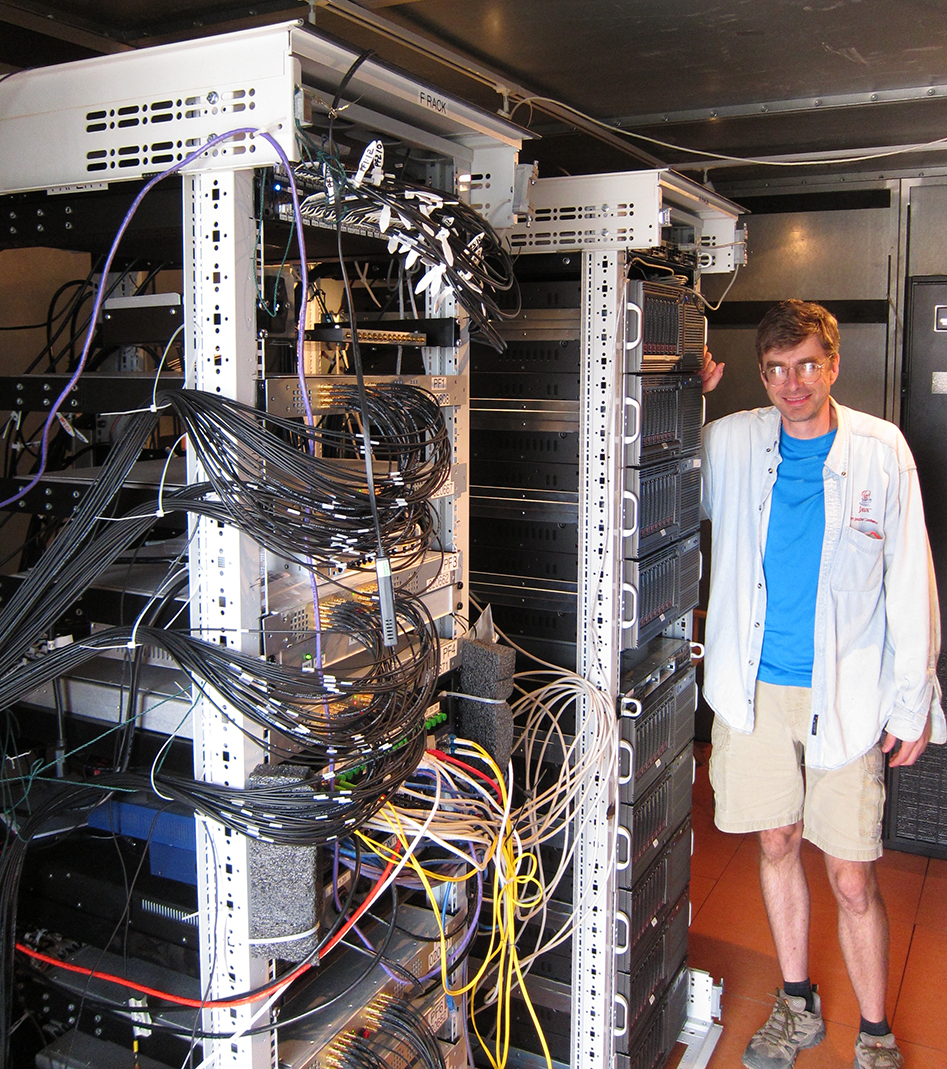
\includegraphics[height=1.5in]{plots/Engineering/digital.png}
    \Caption{-0.1in}{0.9}{-0.1in}{\small
    Existing components re-used in the HERA design include:
    the PAPER dipole antenna (left), 
    receivers in a node module (center), and
    the 128-element correlator deployed in the Karoo (right).
}\label{fig:components}
\end{figure}

HERA's analog signal path inherits directly from PAPER.
In keeping with a philosophy of
incremental change,
HERA-127 reuses the tested and commissioned feed, LNA, cables, and post-amplifier gain modules
(Fig. \ref{fig:components}, left and center) that are currently being
used to good effect in PAPER-128 \Mycitep{parsons_et_al2010}.  Existing PAPER feeds are attached to new
reflector screens that are suspended over the elements, but otherwise remain unmodified.
A parallel development effort an NRAO, aims to improving the feed response below
100 MHz 
and to improve the match between polarization beams in the feed-element system.  
Additional
minor modifications to the analog signal path include transitioning from a 75$\Omega$ to a
shorter 50$\Omega$ cabling system and replacing 100--200 MHz bandpass filters with 50--250 MHz equivalents.
This wider analog bandwidth is used in HERA analysis to improve the extrapolation of smooth foreground
emission over a broader range, and to explore HERA's capability as a Dark-Ages science instrument.
After a Critical Design Review, the results of these development efforts are incorporated in
the transition to the HERA-331 system.  

%The signal is transported to the node via a 35-meter run of 50 $\Omega$ coaxial
%cables. It will terminate on a bulkhead plate on the face of the RFI-tight and
%air-conditioned node. Inside, dual-channel post-amplifier modules (PAMs) (Fig.
%\ref{fig:components}, center) amplify and band-limit the signal. Inside the RFI-tight node,
%the PAMs themselves are housed in RF-shielded boxes.
%


%\subsubsection{Analog System}
%ii. 14m elements + broad band (active) dipole feed
% de Boer, Bradley

\compress
\subsubsection{Digital System}
\label{sec:digital}

\begin{figure}[t]\centering
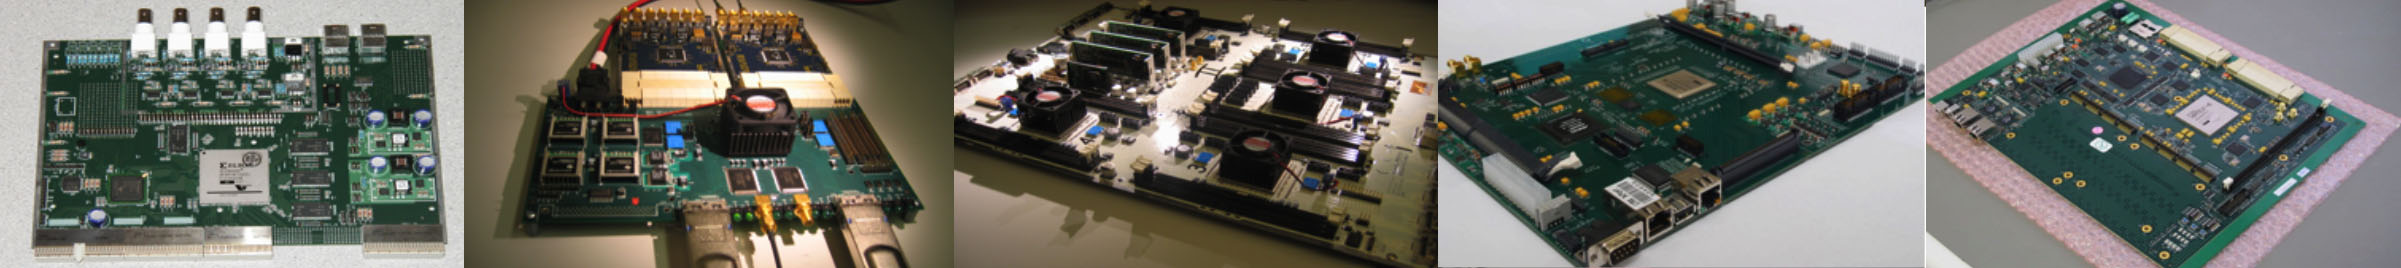
\includegraphics[width=6.5in]{plots/casper_boards.jpg}
\Caption{-0.3in}{0.9}{-0.15in}{\small
Five generations of CASPER technology (progressing left to right) have been used to rapidly
develop, test, and deploy digital instrumentation for radio astronomy.  This technology
allows the PAPER correlator to be 
easily upgraded for HERA, incorporating new technology
\Mycitep{parsons_et_al2006,parsons_et_al2008}.
}\label{fig:casper_boards}
\end{figure}

%HERA's digital system continues in the vein of PAPER's digital correlators.
Although correlators have historically been one of the most complex,
expensive, and risky aspects of developing a radio interferometer, this is no longer the case.
CASPER \citep{parsons_et_al2006}
open-sourced the development of digital signal processing engines for astronomy, and
now has world-wide participation,
with over 500 members at 73 institutions, and 
five generations of hardware (Fig. \ref{fig:casper_boards}). 
On a modest budget, PAPER has applied CASPER technology to develop and deploy new correlators
annually for five years running, each quadrupling the computational capacity of its predecessor.
Led at UC Berkeley's Radio Astronomy Lab (RAL),
HERA efforts continue this incremental development cycle, following a packet-switched
correlator architecture \citep{parsons_et_al2008} that has been
extended in recent PAPER and LEDA deployments (Fig. \ref{fig:components}, right)
to use leverage the computing strengths of both FPGAs and GPUs \citep{clark_et_al2011}.

While HERA-127 uses the existing PAPER correlator directly, for
HERA-331, this correlator architecture will evolve.  As discussed in previous sections,
HERA's science requirements dictate a maximum analog signal path-length.  As a consequence,
digitization needs to happen close to the antenna
elements in the field.  This specification, along with a growing need for modularity to scale with the number of parallel signal paths,
leads HERA to adopt a node-based architecture for amplification, digitization, channelization, and digital
transmission in the field that builds on HERA's MWA heritage.  This architecture is merged with PAPER's clean 
architecture for real-sampling and channelizing the entire analog passband at once, packetizing the data into
10 Gb Ethernet format, and relying on commercial switches to perform the frequency/antenna corner-turn that
FX correlator architectures require. 

%\begin{figure}[t]\centering
%%\includegraphics[width=6.5in]{plots/node_arch.png}
%\caption{
% something about nodes here.  Maybe also block diagram of NRAO digitizer board.
%}\label{fig:node_arch}
%\end{figure}


{\bf Node}. HERA-331 employs RFI-tight node enclosures that each contain the final gain and digitization stages for
signals from 18 antennas, along with power supplies, cooling, and a small server for monitor/control.  
As part of HERA development,
a new board called the Smart Network ADC Processor (SNAP) board is incorporated 
into the CASPER suite of hardware and firmware. This inexpensive board was co-designed by UC Berkeley and NRAO to be
both digitizer and F-engine in HERA's FX correlator architecture,
and is currently in layout at NRAO.  Each SNAP board 
digitizes and channelizes a 50--250 MHz band for 6 input signals (3 antennas, dual-polarization).
A 100-MHz band of selectable channels is transmitted over optical fiber
to a central container (see below), and on to the Karoo Array Processing Building (KAPB).  Development and integration of the SNAP
design and the node system is led at UC Berkeley and after a Critical Design Review, is fabricated
under subcontracts to industry partners in the third project year, and deployed as part of the HERA-331 system.
Development activities under this proposal include porting the CASPER toolflow to
the SNAP board, designing and testing the FPGA firmware,
the integrating and testing of all components in the node subsystem, and providing a monitor/control
access interface.  If time allows, optional development may include doubling the transmitted bandwidth.

{\bf Central Container}.
HERA's central container houses two significant subsystems adjacent to the array.  The first is a timing subsystem
that maintains a GPS-disciplined oscillator and distributes timing
signals (the sampling clock and 1PPS synchronization) to the nodes.  The second
subsystem is a passive fiber optic patch panel that couples
the optical network from the nodes into the 192-filament optical fiber bundle 
that connects to the KAPB. 

{\bf Karoo Array Processing Building (KAPB)}.
The KAPB is currently
in advanced stages of construction for MeerKAT, and houses the switch and processors
that 
complete the HERA correlator system.  The fiber optic bundle that enters the KAPB patch
into local fiber optic cables 
that each terminate in optical transceivers that plug into a 240-port 10 GbE switch.
Such switches, while large, are readily available commercially today.  Also connected to
this switch are 30 servers, each hosting two dual-GPU graphics cards and two dual
10 GbE network interface cards, which implement the cross-multiplication (X-Engine) component
of the correlator during observations.  This estimate for the number of X-Engine servers
is extrapolated from current GPU servers deployed on PAPER, assuming no improvement in bus
speeds for transfering data into the GPU cores, but assuming that the computational
capacity of such GPU cores doubles according to Moore's Law prior to the purchase of
these servers in the third year of the project.
Output data from the correlator are written to the data storage system described
in the following section.

%C. Post correlator data path
% Aguirre, Moore

\compress
\subsubsection{Data Storage, Compression, Transfer, and Computing}
\label{sec:data}

HERA's data management system is responsible for recording raw data from the
correlator, compressing that data in real-time, applying routine calibration
and analysis pipelines, and transferring data products to 
a high-performance computing cluster at UPenn.
UPenn leads the procurement
and deployment of three data storage systems:
\begin{itemize}[noitemsep,nolistsep]
\item a 1.5 PB system deployed in the KAPB for archiving all 1.2 PB of raw data and 60 TB of compressed data, 
\item 6 network attached storage (NAS) units plus 2 125 TB RAID array units that are used to ship compressed data products to the US, and
\item a permanent 250 TB system at UPenn associated with a computing cluster that
holds compressed data products and serves as the analysis engine for HERA collaborators.
\end{itemize}
\noindent
This effort leverages existing infrastructure at UPenn, with support
for the expansion of the data storage and for upgrading to a 30-node computing cluster.  This cluster supports the bulk of the analysis by HERA collaborators (see \S\ref{sec:analysis}) that requires access to the full set of HERA observations.

%The main data center at Penn will house all of the maximally compressed data from all seasons of HERA, as well as the LST-averaged data.  The storage system is sized so that there is a factor of 4 overhead for work on the maximally-compressed data set, and a factor of 2 on the LST-averaged. The 500 TB data storage will be coupled to a 32-node cluster which performs the tasks of calibration and averaging to further reduce the data volume.  This cluster will support the bulk of the analysis requiring the full data set.  Subsets will be served off to collaborators from this system.  The entire data storage and transfer plan for HERA draws heavily on the experience with PAPER data.

The data compression scheme at the heart of the data management system
has been implemented for PAPER (\Mycitealt{parsons_et_al2013},
Appendix A), and is applied to HERA visibilities to reduce data volume by
a factor of $\sim$20 without impacting reionization science
capabilities.  This compression technique, which is based on delay/delay-rate
filtering \Mycitep{parsons_backer2009}, is applied uniformly to all visibilities
in the array, does not require (or produce) detailed calibration
information, and is minimally restrictive for how data are analyzed and calibrated afterward.
Data compression is run on the same GPU servers
that implement the correlator X-Engines (\S\ref{sec:digital}).  Since HERA only observes at night,
these processors would otherwise be unused.  UC Berkeley is responsible for porting
the existing data compression pipeline to target these servers.

Data quality assurance (QA) is performed in real time on an additional modest 
computing cluster in the
KAPB.  UPenn leads the deployment and support of the hardware system that
manages data transfer, applies routine calibration pipelines (see \S\ref{sec:analysis}) and quality
checks, and aggregates correlation-based metrics of array performance in real-time.  The QA system
furnishes this information into the separate monitor and control system (\S\ref{sec:monitor}).
A modest amount of data transfer is possible over the internet; PAPER's data transfer rate from the Karoo
to UPenn varies, but peaks around 40 Mbps.  The QA system drives internet data transfer, but
NAS devices and RAID storage, transferred by air-freight shipping, ensure full data transfer to UPenn.

%ii. transport to data centers
%In order to transfer maximally-compressed data over the internet in a timely manner, a network speed of around the instantaneous compressed data rate is required.  Negotiations with the IT SKASA and the South African internet provider (Tenet) have achieved transfer speeds between the PAPER site and the United States have been measured to be up to 40 Mbps, which easily
%accommodates the first two seasons of HERA observations.  In all seasons, however, portable, inexpensive, network-attached storage devices will be used to transfer data by air-freight shipping. 

%iii. data centers: access?

%The main data center at Penn will house all of the maximally compressed data from all seasons of HERA, as well as the LST-averaged data.  The storage system is sized so that there is a factor of 4 overhead for work on the maximally-compressed data set, and a factor of 2 on the LST-averaged. The 500 TB data storage will be coupled to a 32-node cluster which performs the tasks of calibration and averaging to further reduce the data volume.  This cluster will support the bulk of the analysis requiring the full data set.  Subsets will be served off to collaborators from this system.  The entire data storage and transfer plan for HERA draws heavily on the experience with PAPER data.

\compress
\subsubsection{Monitor and Control}
\label{sec:monitor}

The U. of Washington team leads the development of HERA's Monitor and Control (M\&C) system,
which is a straightforward port of a similar system used on the MWA \citep{tingay_et_al2013}.
This system is
responsible for tracking observing status, array startup and shutdown, and
monitoring of all active HERA systems. In the process, the M\&C system builds a sizeable database of 
metadata that is crucial for verifying system functionality, identifying hardware failures, and feeding
calibration and contextual information into data analysis pipelines.  

%Top-level interface for controlling and monitoring major subsystems. 
%Collection of monitor data from nodes, switch, correlator, data compression, and data transfer subsystems.
%Incorporation of calibration data from real-time application of redundant calibration (cite section), as well as
%other calibration, imaging, and assessment subsystems.
%
%%\subsubsection{Array monitoring/maintenance: daily, weekly health monitoring}
%% de Boer
%
%In addition to Monitor and Control subsystem, which aggregates routine checks that are run automatically as
%part of the data compression and transfer pipeline, there is a need for deeper analysis
%exploring the data for more subtle defects, as well as monitoring progress toward sensitivity goals.
%We have set aside time for students at each institution, rotating among institutions, and managed at MIT,
%for performing such data exercises.
%Combine this with information from monitor database to identify hardware and subsystem failures.
%Aggregate lists of systems requiring maintenance attention, which are then handled by system owners
%in coordination with appropriate members of their teams.

%\vspace{-0.25in}
%\subsection{Prototype Construction and Testing}
%\vspace{-6pt}
%
%One prototype of the antenna has been constructed near the Radio Astronomy Lab in California. 
%This prototype serves as an important first construction test-bed and is currently being used to do 
%initial network analyzer measurements (Fig. \ref{fig:heracles}).
%This proposal calls for the construction of two additional prototype dishes alongside
%the PAPER array deployed at the NRAO site near Green Bank, WV.
%These dishes will be tested
%with a network analyzer in situ, and will be cross-correlated with PAPER elements using
%the correlator currently deployed on site, in order to measure
%the element performance and optimize the design.  The goal of this effort is to ensure
%that all signal reflections
%are attenuated by a factor of -60 dB by the time that they are capable of entering the signal path
%at a delays greater than 50 ns.  While signal reflections will be inevitable with such a dish
%design, the quality of the impedance match at the feed,
%the presence of structures that reduces resonances between
%the feed and the dish, and control of the focal height of the parabola are all aspects
%of the design that can
%be manipulated to help achieve this specification, ensuring that reionization modes above
%$k_\parallel=0.1h {\rm Mpc}^{-1}$ are not dominated by foreground contamination.
%
%
%These additional prototypes will be important to finalize the specific construction techniques to be 
%used in the final antenna construction contract in South Africa.

\vspace{-0.25in}
\subsection{Array Construction and Commissioning}
\vspace{-6pt}

Construction of HERA elements in the array consists of five primary steps: 
(1) site preparation and surveying, (2) pole installation by contracted labor with specialized utility pole equipment,
(3) hub placement and height adjustment, (4) construction of full element using local labor,
and (5) migration of PAPER dipoles to new ground screens by project staff.
Contractors and immediate supervisors are based in South Africa.  Supervision staff 
are part of the extensive support infrastructure in place on site associated with South African SKA activities.
%As mentioned above, the tall poles are shared amongst the antennas in the tight configuration.  
%These are standard telephone/power 
%utility poles and a great deal of  expertise and infrastructure exists to install these in remote settings.  
%Figure \ref{fig:hera_dish} (right) shows hexagonal antenna configuration, including the tall pole locations.
%The right panel shows a cross-section of an element.
The PVC and wood sub-assemblies 
are constructed under contract off-site where material and labor are readily accessible.  After being and shipped to site, the
remaining construction involving sub-assemblies, pre-cut wood, PVC, and pre-cut wire cloth 
is done on-site under contract.  

%\begin{figure}[h]
%	\centering
%		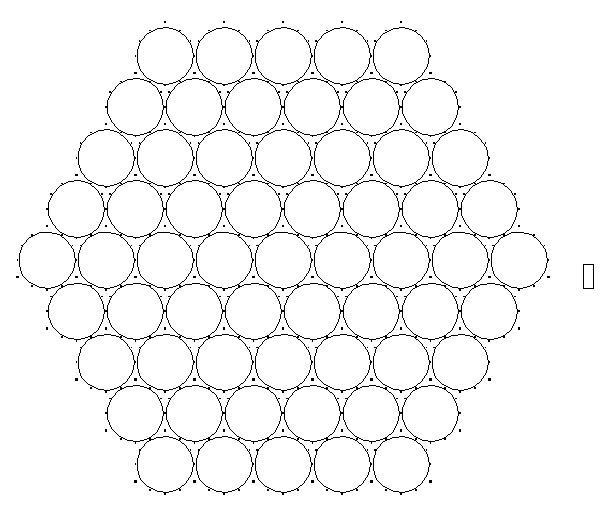
\includegraphics[width=0.35\textwidth]{plots/Engineering/hex_61.png} 
%		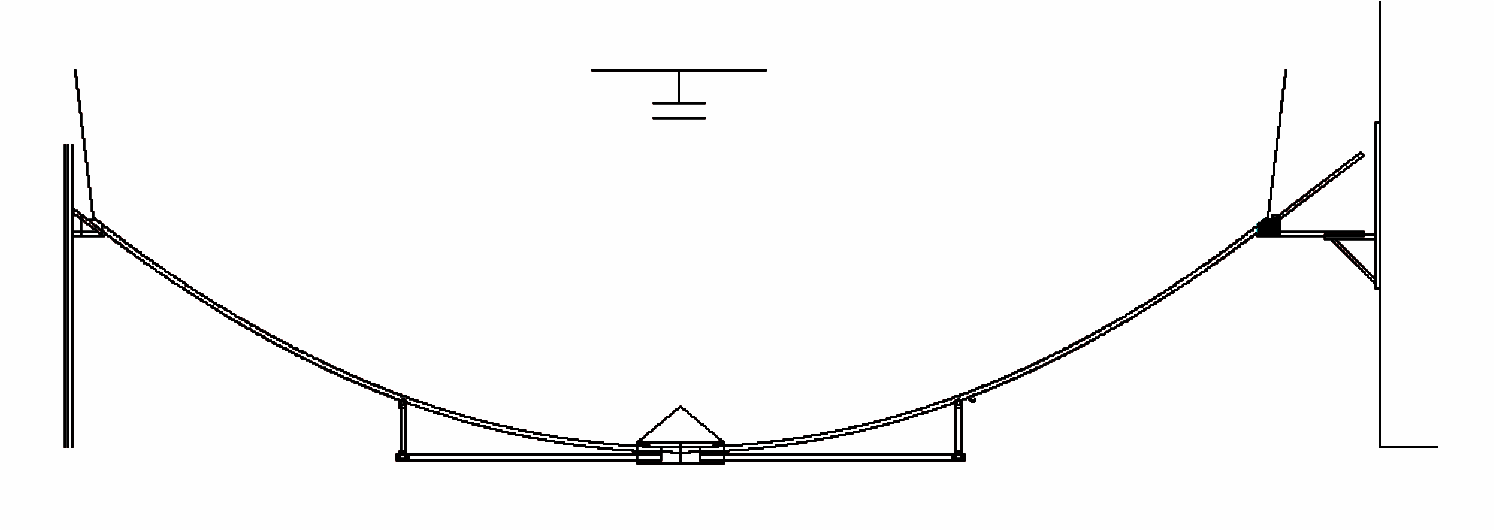
\includegraphics[width=0.6\textwidth]{plots/Engineering/optics.png}
%\caption{\small
%Left: the configuration of the 331-element array.  Note the rectangular container to scale on right.
%		Right: a cross-section and optics of an element.}
%	\label{fig:config_optics}
%\end{figure}
%Except for two custom metal assemblies, the remainder of the construction materials are standard wood, 
%metal and PVC parts.  The two custom assemblies are simple small welded metal assemblies for the end of 
%rim support pieces (quantity 12) and the feed and feed backplane (quantity 1).  

%\subsection{Commissioning}

As construction proceeds incrementally, project staff begin migrating over existing PAPER feeds and cables 
and start commissioning the array.  
Commissioning activities are led first by subsystem owners, verifying that deployed subsystems 
continue to pass the test suites developed for the Critical Design Review.
As the focus moves to system-level integration processes, downstream subsystems increasingly
lead commissioning efforts until a subset of the HERA
array has been fully integrated and tested.  Once a baseline of functionality is established,
more antennas and upgraded subsystems can be incorporated incrementally as they are available.
These commissioning activities follow the successful
build/commission model used by both PAPER and MWA, % The PAPER team has
%commissioned 7 unique arrays, each with different correlators and
%configurations while the MWA, a much larger system designed for many
%operational modes, was successfully commissioned on schedule during a single
%coordinated effort.  
where observers tracked the incremental build-out
process, performed observations in a ``science-like mode,'' and made
adjustments as needed. 
%The resulting modifications during this period resulted
%in dramatically improved instrument performance.  

More advanced commisioning tasks involve all institutions, and
focus on meeting top-level science requirements
and resulting specifications.  %The most important of these are maximizing
%up-time, decreasing time-to-science, and optimizing for reionization science.
These tasks exercise the Monitor and Control subsystem (M\&C; \S\ref{sec:monitor})
and the Quality Assurance data processor (QA; \S\ref{sec:data}), 
aggregating sources of
information about array heaolth from all subsystems and providing an accurate
state of the system report visible and understandable to the entire project.
Tests and pipelines developed during commissioning are folded into
the routine analysis that reports to the M\&C system.  As systems stabilize,
useful post-processing steps such as redundancy-based calibration and automated
imaging are incorporated into the on-site QA server.
%that is specifically for this purpose.

%Optimization for reionization science is achieved by making and reducing early
%science observations. This process includes many critical projects, such
%complex gain calibration (using redundancy and sky models), mapping of the beam
%pattern by comparison with PAPER elements and catalogs, establishing an
%absolute calibration, making images, cataloging visible sources. Crucially, it
%includes measuring signal reflections, cross-couplings and other possible
%artifacts using power spectrum analysis techniques. The end result will be an
%ongoing program of online deep integrations that will provide a near-real-time
%high-sensitivity delay spectrum verifying the absence of low-level reflections
%in the reionization window.


\compress
\subsection{Software, Analysis, and Science}
\label{sec:analysis}

Beyond the construction and data-taking aspects of HERA, this proposal
incorporates a full data analysis effort, culminating in the publication of a
suite of science papers connecting observations to the physics of cosmic dawn.
These efforts leverage existing software pipelines, with on-going 
development driven by students and postdocs targeting specific science goals.
On the science side, HERA leverages the involvement of a team theory collaborators,
including Furlanetto, Lidz, Loeb, McQuinn, Mesinger, Oh, Pritchard, Santos, and Sutter.

%\compress
%\subsubsection{Calibration}
%\label{sec:calibration} 

{\bf Calibration and Snapshot Imaging}. MIT leads
the development of a real-time redundancy-based calibration pipeline based on related
MITEoR and PAPER efforts.
These instantaneous calibration solutions are provided to
the Monitor and Control system to enable 
hardware misbehaviors to be quickly identified, and also support the
real-time imaging pipeline.  Absolute calibration is fixed with
a combination of self-calibration techniques and absolutely calibrated baluns developed at ASU and NRAO.
%Once data quality is assured, multi-day observations 
%binned in local sidereal time, and averaged. This intermediate
%averaging scheme will also generate an accurate visibility-based sky
%model for the instrument once calibration is applied.
Offline, detailed imaging efforts feed into developiing
empirical beam models that
complement electromagnetic simulations.  UPenn develops polarization beam models
that determine whether polarization leakage can be formally retired as 
a risk, and lay the foundation for imaging-based foreground suppression that
corrects any remaining leakage effects.

%\compress
%\subsubsection{Foreground Modeling and Removal}
%\label{sec:DataProducts}

{\bf Foreground Modeling}. The U. Washington team leads the adaptation
of a high dynamic-range imaging pipeline
based on the Fast Holographic Deconvolution (FHD; \citealt{sullivan_et_al2012}).
for HERA.  The full-Stokes sky maps resulting from this pipeline
are used to directly subtract foregrounds,
and as data products themselves.  UPenn leads
the characterization of the polarized sky and the
distribution of rotation measures.  Data from HERA, PAPER, and the MWA are used
to update source catalogs and a Global
Sky Model \citep{deoliveira2008}. %providing reference sky models for both
%HERA and other low-frequency instruments. %The goal will be to generate a model
%suitable for direct subtraction of foregrounds. 

% XXX need more data products here

%\compress
%\subsubsection{Power spectrum and related measurements}

{\bf Power Spectra}. UC Berkeley leads early power spectrum measurements using the conservative
delay-spectrum approach used in PAPER.  %This
%visibility-based approach, when coupled with a foreground-avoidance strategy,
%is sufficient for an unambiguous early detection of the 21~cm
%power spectrum should results from current-generation experiments prove
%marginal (Fig. \ref{fig:eor_pspec} and Table \ref{tab:signif}).  
Development of
the power-spectrum pipeline will focus on incorporating
a fully covariant description of the foreground wedge
\citep{liu_tegmark2011,dillon_et_al2013a}, as well as
exploring Bayesian techniques for power spectrum estimation, building on the considerable
progress already made on Gibbs-sampling imaging for interferometers \citep{sutter_et_al2014}.
In addition to the statistical foreground mitigation techniques provided by optimal quatratic
power-spectrum estimation, U. Washington leads the application of 
foreground modeling for expanding the range of modes available for power spectrum analysis.
Techniques developed should be equally applicable
to measurements in both the reionization epoch and at higher redshifts.  MIT leads the application
of these tools for pre-reionization science.

{\bf Simulation}. To provide verification of power spectrum constraints, ASU leads the
development an end-to-end simulator of the full HERA instrument, incorporating
foregrounds and reionization models to output visibilities.  UCLA also leads
a parametrized reionization simulation effort that, coupled with the instrument
simulator, is critical for connecting power-spectrum constraints to the estimating
of the underlying astrophysical models.

%\compress
%\subsubsection{HI Imaging}

{\bf HI Imaging}. In addition to supplying models for suppressing foregrounds,
deep imaging aims to map HI emission during reionization (see \S\ref{sec:science}).
Initially, conservative filtering of the foreground wedge is applied to data that
are imaged.  These results are compared with the residuals from imaging-based
foreground suppression to explore the limitations of 
precision foreground imaging and removal.  The imaging-based techniques mature, the resultant
maps are released for cross-correlation with other probes of reionization.

%\subsubsection{Aspirations [move to facilities section?]}
%
%i. FFT correlator
%ii. other


%\compress
%\subsection{Schedule} % 0.5 page
% De Boer


%\begin{table}[t]
%\centering
%\caption{Schedule Overview}
%\label{tab:scheduleSummary}
%\begin{tabular}{| p{1.5in} | p{1.5in} | p{1.5in} | p{1.5in} |}\hline
%\textbf{Year 1}:  FY2015   &  \textbf{Year 2}:  FY2016  &  \textbf{Year 3}:  FY2017 & \textbf{Year 4}:  FY2018 \\ \hline
%\raggedright{Infrastructure, prototyping and contract preparation.} &
%\raggedright{Hardware commissioning and deep foreground survey.} &
%\raggedright{HERA-127 observations:  detecting the rise and fall of reionization.} &
%HERA-331 observations:  measuring the evolution of the first galaxies. \\ \hline  %It won't let me make this one raggedright!
%\begin{itemize}[noitemsep,nolistsep,leftmargin=12pt]
%\item Basic infrastructure
%\item GB, SA prototypes
%\item Design package
%\item Polarization software
%\end{itemize} &
%\begin{itemize}[noitemsep,nolistsep,leftmargin=12pt]
%\item HERA beam pattern
%\item HERA-127
%\item Delay-spectrum/FHD software
%\item Analysis pipelines
%\end{itemize} &
%\begin{itemize}[noitemsep,nolistsep,leftmargin=12pt]
%\item HERA-127 observations
%\item Electronics upgrade
%\item HERA-331
%\item HERA-127 analysis
%\end{itemize} &
%\begin{itemize}[noitemsep,nolistsep,leftmargin=12pt]
%\item HERA-331 observations
%\item Cross-correlations
%\item Cosmological simulations
%\end{itemize} \\ \hline
%\end{tabular}
%\end{table}

% need to discuss in a few sentences the
% relation to other experiments in the same time frame.

%\begin{itemize}[noitemsep,nolistsep]
%\item{Year 1:} Infrastructure, Prototyping, Contract Preparation (FY 2015).      
%\begin{itemize}[noitemsep,nolistsep]
%\item Install basic infrastructure (ground leveling, power, network connectivity) for new infrastructure
%\item Incorporate existing PAPER-128 antennas, correlator, and housing container.
%\item Install additional prototypes in Green Bank and test.
%\item Define final design package for element construction
%\item Start developing improved HERA baluns, receivers, feeds, nodes, and in-situ antenna calibration system.
%\item Continue delay-spectrum, FHD, and optimal estimator software development.
%\item Develop polarization capable software for beam/leakage studies.
%\end{itemize}
%\item{Year 2:} Hardware Commissioning and Deep Foreground Survey (FY 2016).  
%\begin{itemize}[noitemsep,nolistsep]
%\item Observations using PAPER antennas in an imaging configuration.
%\item Determine on-sky beam response of HERA antennas to facilitate future source subtraction efforts.
%\item Finalize site infrastructure (high-bandwidth optical network, surveying, trenching).
%\item Commission new feeds, receivers, nodes, and calibration systems in Green Bank and SA.
%\item Complete HERA-127 construction
%\item Initial delay-spectrum, FHD, and optimal estimator software ready for HERA 127 analysis.
%\item Full end-to-end simulations of analysis pipelines.
%\end{itemize}
%\item{Year 3:} HERA 127 and Detecting the Rise and Fall of Reionization (FY 2017).  
%\begin{itemize}[noitemsep,nolistsep]
%\item HERA 127 complete. Science observations begin using the PAPER correlator.
%\item Begin deployment of HERA 331. Install new node electronics and a 331-element, GPU-based correlator in the Karoo Array Processing Building (KAPB).
%\item Install new data storage infrastructure in the KAPB.
%\item Upgrade the UPenn analysis cluster.
%\item Finish construction of HERA 331
%\item Apply proven delay-spectrum analysis techniques to HERA 127 observations to constrain the timing and duration of reionization.
%\item Multi-pipeline analysis of HERA 127 observations to compare pipeline strengths/weaknesses.
%\end{itemize}
%\item{Year 4:} HERA 331 and Measuring the Evolution of the First Galaxies (FY 2018).           
%\begin{itemize}[noitemsep,nolistsep]
%\item HERA 331 complete. Begin science observations Oct. 2017.\item Begin multi-pipeline analysis of data to characterize the evolution of the power spectrum and determining properties of the first galaxies. 
%\item Continue analysis software development: optimize existing algorithms and develop imaging-based subtraction techniques for expanding the EoR window
%\item Create high-fidelity maps/data cubes of the HERA field for cross-correlation studies
%\item Cosmological simulations for extracting reionization physics from power spectrum measurements
%\end{itemize}
%\end{itemize}

%  ___                  _           ___                     _      
% | _ )_ _ ___  __ _ __| |___ _ _  |_ _|_ __  _ __  __ _ __| |_ ___
% | _ \ '_/ _ \/ _` / _` / -_) '_|  | || '  \| '_ \/ _` / _|  _(_-<
% |___/_| \___/\__,_\__,_\___|_|   |___|_|_|_| .__/\__,_\__|\__/__/
%                                            |_|        

\compress
\section{Broader Impacts} % 1 page
% Aguirre

At the core
of HERA's plan to broaden its impact
is an international scientific collaboration and student
exchange program with South Africa.  We also continue the PAPER
and MWA legacy of training new scientists and engineers at the graduate,
undergraduate levels, postdoctoral levels.  We make major data products
available publicly as a benefit to the community, and help to define the
science context and techniques for the next generation of experiments ---
particularly the SKA.

\compress
\subsection{South African Student Exchange}

We propose 
a student exchange program
between HERA and South African scientific collaborators,
building on the existing
collaboration between PAPER, CASPER, SKA-SA, and South African universities.
We have identified several collaborators at SA institutions (see attached
letters of support from Bernardi (SKA-SA); Chiang, Moodley, and 
Sievers (UKZN)).  This exchange is mutually beneficial,
preparing students on both sides as scientific and engineering leaders
in next-generation 21~cm
reionization experiments and the SKA.  This
exchange increases the size, diversity, and quality of US graduate programs by
engaging and preparing South African students for admission to US institutions,
and by exposing US students to the burgeoning radio astronomy facilities being
developed in South Africa as part of the SKA. %Both scientific and engineering
%exchanges are part of this program.  

Each year,
3--4 students from the USA and SA 
travel to a rotating host institution to work on a related set of
research problems.  
Experience has shown that small groups facilitate peer mentoring and
a sense of community, particularly when operating in a new cultural
environment.  A similar approach is taken for South African students
in the National Astrophysics and Space Science Programme (NASSP)
%; http://www.star.ac.za/) 
and also in US programs (e.g., the Posse Foundation).
%http://www.possefoundation.org/).  
Over a three-month period,
students interact with their host institution's
faculty, postdocs, and graduate students.  Budget
allowance includes travel, lodging, and meals.  Master's students 
are mentored for applying to Ph.D. programs and engineering positions.  Doctoral
candidates participate in multiple exchanges, 
establishing a scientific presence in their host country for
building collaborations, applying for postdoctoral or permanent
positions, and using the host
country's astronomy facilities.  %In order to vary the experience, each
%year targets a different host institution on each side.

This outreach program draws from an existing pool of talent, 
leveraging SKA-SA's standing commitment to aiding previously disadvantaged South Africans,
which prioritizes support to black and women South Africans at undergraduate level,
identifying non-traditional students, and guiding and supporting them into
higher levels of research.  
%The level of financial support provided by SKA-SA at all levels of study and
%research ensure that the students do not have to concern themselves with
%finding employment immediately after graduating from a degree, a problem faced
%by many students who have obligations to contribute to their families’ income.
Special attention is paid to bridging issues of
scientific culture, allowing both groups to function at the highest possible
level within their exchange community.  We anticipate that this program will
prepare students on both sides to be able to productively apply for graduate,
postdoctoral, and faculty positions in the exchange country, and to effectively
apply for observing time on the SKA and NRAO facilities.  

\compress
\subsection{Additional Broader Impacts and Previous Results}
\label{sec:other_broader}

%A. pre and post-doctoral students
%\subsection{Student Education}
%proposals must include, and will be evaluated on, a substantial component of
%student training and involvement of a diverse and inclusive workforce in
%instrumentation, facility development, or data management/analysis.

With each institution contributing subsystems to HERA,
students and postdocs at all institutions take a leading role in development,
testing, deployment, commissioning, and observing.
This continues the HERA collaboration's commitment to
training a diverse set of students to become next-generation leaders in science.  
A prime example of this is CASPER, which began as the core of PAPER's digital development effort,
recruiting undergraduates, interns, grad students, and
postdocs to work alongside seasoned RAL veteran engineers in a laboratory setting.
CASPER now supports a global community of instrumentalists with
a broad range of tools, including mailing lists, student
visits, annual workshops, and an online repository of documentation and pedagogical materials.
While grant support for CASPER at UC Berkeley has expired, this community continues to look
to UC Berkeley's leadership.  Part of HERA's broader impact continues
this legacy, adapting technology developed for HERA for broader use in the CASPER community, 
hosting the workshops that help define this community, and continuing to recruit bright
young students to develop novel approaches to scientific instrumentation.
%has helped rebeen a powerful recruiting tool, bringing students to work from
%South Africa (Manley), and beginning the career of the PI, Parsons, as well as
%current graduate students (Ali, Zheng).  
%Recruiting of engineering students into science.  Focus on both development,
%testing, and documentation phases of instrument development.  Involvement in
%design reviews.  Harnessing energy of young students, combining with the
%stability and discipline.
%Such recruitment is enabled by a broad range of tools, including mailing lists, student
%visits, and workshops, which have disseminated
%engineering expertise to a community much broader even than the set of students and
%engineers supported under this proposal. 
%Annual workshops.  Hosting visiting students (reference next section). Cite
%past cases: Manley, Landon, Zhang (Omniscope).  Mention specific success cases
%in progressing careers of instrumentalists: Parsons, Siemion, Ali, Hsyu,
%Leung, etc.

%While UC Berkeley leads core instrument development and construction,
%each institution contributes necessary instrumentation, computing,
%monitor/control, data management, and analysis software to the project.  
%Students and postdocs at all institutions take a leading role in development and
%testing (participating in critical design reviews), and 
%contribute to deployment, commissioning, and observing.

HERA builds on a long history of student training, career development, and public outreach.
PAPER and the MWA have
included undergraduate, graduate, and postdoctoral researchers in all
phases of design, construction, and analysis.  The combined efforts of these
groups have trained an impressive cadre of scientists skilled in
instrumentation, data analysis, and theory, as well as engineers working at the
forefront of digital technology.
MITEoR has placed seven physics undergrads 
in competitve graduate schools. over a dozen interns from South African
universities have received academic credit for participating in 
PAPER's major engineering deployments.
%astronomy); 
 Furlanetto (UCLA)
%at UCLA 
has led two summer REU projects, and has
% This project [same one listed above] supported Dixon during part of her PhD
% thesis work and Mesinger during his first postdoctoral fellowship. It also
% led to two summer REU projects (though no support was required from the
% grant, thanks to the UCLA REU program) for Samuel Johnson Stoever (then at
% Cornell) and Fred Davies (then at New Mexico Tech, now one of the PI's
% graduate students).  Furlanetto also 
presented his work to three astronomy clubs in the LA area. %and at more than a
%dozen astronomy and physics colloquia and invited talks.   
Aguirre's (Penn)
numerous undergraduate and high-school students working on PAPER
include an Acorda Scientific Excellence Awardee.
Parsons (UCB) routinely produces
public (YouTube) pedagogical videos for undergraduate teaching, and has established
an internship program for training budding instrumentalists.
Morales (UW) was honored by Diversity Magazine as an 
emerging minority scholar, was featured in the Pacific Science
Center’s ``Scientists Like Me: Faces of Discovery'', and has
implemented a successful community college transfer program. 
Bowman and Jacobs (ASU) are actively involved in community outreach at
local urban schools and tribal centers. Hewitt (MIT) has a long history of advocating
for women in science and helped establish
family leave policies for young faculty.
Tegmark (MIT) has reached a wide lay audience through his popular book,
``Our Mathematical Universe" (New York Times Bestseller's List, Jan. 2014),
which includes sections on radio instrumentation and 21~cm cosmology.

%{\it We have and will provide benefits to the astronomical community}

HERA collaborators have a strong record of sharing breakthrough
innovations with the wider scientific and engineering communities, distributing 
open-source software (AIPY, DexM), hardware and firmware (CASPER), 
and instrument architectures (PAPER, LEDA, Omniscope),
publishing innovative analysis approaches (FHD, MOFF,
Omniscope), and serving in leadership roles for major international communities (SKA, ASKAP, ALMA, MeerKat, Chime).  
While HERA is an experiment rather than an observatory, its
results are scientifically and technologically relevant for the
SKA, and for high-redshift observing with JWST and ALMA.
%Our benefit to the wider community is: 1. answering important question that is
%relevant to broader community studying first galaxies, 2. set science context
%for SKA, 3. develop techniques for SKA Cite high rate of adoption of CASPER
%hardware in the community.  Delivering a next generation of signal processing
%platform.  Development of heterogeneous computing systems involving CPUs,
%GPUs, and FPGAs, including DSP libraries, data handling, and control software.
%Sharing of LEDA GPU code \citep{clark_et_al2011} with PAPER's FPGA processors,
%data handling, and control software.  Continued support and development for
%the benefit of the radio astronomy instrumentation community.
As detailed in the Data Management Plan, HERA's data products are made available to the wider
community for a variety of studies, both those directly
relevant to cosmic dawn, and other topics, such as transient studies. 

%  ___                __ _ _      
% | _ ) ___ _ _  ___ / _(_) |_ ___
% | _ \/ -_) ' \/ -_)  _| |  _(_-<
% |___/\___|_||_\___|_| |_|\__/__/

%\compress
%\subsection{Impacts to the Astronomical Community}
%\subsection{Impacts for the Broader Astronomy Community}

% This probably belongs in the Data Management Plan

%i. Data access: transients, SETI, ionosphere
% The HERA measurements will be released to the community after an 18-month proprietary period and hosted on a public server at MIT (see \S\ref{sec:DataProducts}).  A large number of data products will be available.  Imaging products will include coarse real-time calibrated snapshot images in addition to high dynamic range survey maps from the FHD pipeline.  Calibrated, compressed, LST-binned visibilities will also be made public for re-analysis.  Higher cadence data sets will not be hosted publicly in a continuous fashion due to data transfer limitations, but will be available to any users upon request.  A number of derived data products will also be made accessible.  Source catalogs will be provided, and a Global Sky Model of diffuse foregrounds will be updated with new observations and released.  Foreground-subtracted data cubes of high-redshift $21\,\textrm{cm}$ intensity maps and the associated ionization field will be available for cross-correlation studies, as well as to provide context for high 
% redshift optical and IR studies.





% ii. Cross correlation: CMBpol, CO/CII IM
%On the HERA timescale, a number of new observations will come online that would benefit from cross-comparison with the power spectra and images produced by HERA (see Section \ref{sec:science}). For example, HERA will provide the large-scale reionization environment for pointed JWST or ALMA galaxy observations and can offer cross-correlations with  the WFIRST near-IR surveys \citep{lidz_et_al2009}.
 
%  ___                                
% / __|_  _ _ __  _ __  __ _ _ _ _  _ 
% \__ \ || | '  \| '  \/ _` | '_| || |
% |___/\_,_|_|_|_|_|_|_\__,_|_|  \_, |
%                                |__/ 

\compress
\section{Summary} % 0.5 pages
% Parsons

%This HERA proposal follows the vision for 21~cm observations laid out in NWNH.
%PAPER and the MWA have already succeeded in the primary task envisioned in
%NWNH---characterizing the astrophysical foregrounds and developing the hardware
%and analysis tools needed to suppress the contamination. The discovery and
%characterization of the EoR Window and the development of precision foreground
%mitigation techniques have shown that foregrounds can be suppressed to the current
%thermal noise level (\S \ref{sec:Lessons}; \citealt{parsons_et_al2013}). While the MWA,
%PAPER, and LOFAR are pushing hard to detect the EoR power spectrum,
%a marginal detection is the best these instruments are likely to achieve.
%HERA will both ensure a high significance detection of the \HI 21~cm  signal as
%well as provide powerful constraints on the rise and fall of reionization \citep{pober_et_al2014}, how
%early stars and structure formed, and which physical processes dominated heating at the end of the
%cosmic dark ages (Figs. \ref{fig:x_i_vs_z} \& \ref{fig:eor_pspec}).
%
%As envisioned in NWNH, the US EoR projects (PAPER, MWA, EDGES, MITEoR) have
%pooled their expertise to develop the second generation HERA experiment. This
%has created a collaborative team with a deep well of scientific
%experience---the majority of papers on EoR observations are authored by members
%of the HERA team. By leveraging this expertise, the HERA design is significantly
%less expensive than envisioned in 
%NWNH and has greater scientific reach.
%
%The last few years have been remarkably productive---we
%understand foreground systematics and are pushing existing
%instruments to their thermal limits. We are now ready to build the HERA
%instrument envisioned in NWNH and realize the scientific promise of 21~cm
%cosmology. Studying the formation of the first luminous structures 
%and how they reionize the Universe is a primary driver for 
%nearly all major astronomical facilities over the next decade.
%Such studies include direct  observations of stars, gas, dust, and AGN in the
%first galaxies using the JWST, TMT, and ALMA. HERA is 
%a necessary element in this panchromatic arsenal, 
%providing a unique window onto the impact of these sources on 
%their large-scale environments.

This HERA proposal follows the vision for 21~cm observations laid out in NWNH,
with the US EoR projects (PAPER, MWA, EDGES, MITEoR) pooling their expertise to
develop a second-generation instrument.  The resulting team comes with a deep
well of scientific experience --- the majority of papers on EoR observations
are written by the HERA team.
%XXX JCP: is this true?  certainly US papers on EoR observations... but counting GMRT & LOFAR, I wager not.
This expertise has led to rapid progress in the last few years, with current
instruments having fulfilled their primary goal envisioned in NWNH:
characterizing and suppressing astrophysical foregrounds through hardware and
analysis development, to the point where thermal noise limits have been
reached.  MWA, PAPER, and LOFAR are now pushing hard to detect the EoR power
spectrum, but at best, the detection will be marginal.  Through judicious
leveraging of the EoR window and related foreground mitigation techniques, HERA
not only ensures a high significance detection of the \HI 21~cm signal, but
also provides strong constraints on the reionization history,
early structure formation, and heating processes at
the end of the cosmic dark ages.
%As stands, there is a broad gap in scale and scientific maturity between
%current experiments and what should be required for future efforts such as
%HERA-III and SKA-low.  This proposal fills this gap, building on the lessons learned
%from current-generation experiments, validating techniques for accessing
%the 21~cm reionization signal, and moving beyond first detection to 
%learning about the astrophysics of reionization.  
This proposal comes at an
opportune time in the field, picking up where PAPER, the MWA, and LOFAR leave
off, and delivering results on a timescale that ensures continued US leadership in the field.

Studying the formation of the first luminous structures 
and how they reionize the Universe is a primary driver for 
nearly all major astronomical facilities over the next decade.
Such studies include direct  observations of stars, gas, dust, and AGN in the
first galaxies using the JWST, TMT, and ALMA. HERA is 
a necessary element in this panchromatic arsenal, 
providing a unique window onto the impact of these sources on 
their large-scale environments.


\clearpage
\setcounter{page}{1}
\thispagestyle{empty}
%\bibliographystyle{apj}
%\bibliographystyle{hapj}
\bibliographystyle{jponew}
%\bibliography{proj_description}
\bibliography{biblio}

\end{document}

